\documentclass[oneside, a4paper,11pt]{book}
\usepackage[margin=1in]{geometry}

\usepackage{graphicx}
\usepackage[utf8]{inputenc} % allow utf-8 input
\usepackage[T1]{fontenc}    % use 8-bit T1 fonts
\usepackage{hyperref}       % hyperlinks
\usepackage{url}            % simple URL typesetting
\usepackage{booktabs}       % professional-quality tables
\usepackage{nicefrac}       % compact symbols for 1/2, etc.
\usepackage{microtype}      % microtypography

\usepackage{listings}
\usepackage{xcolor}
\definecolor{codegreen}{rgb}{0,0.6,0}
\definecolor{codegray}{rgb}{0.5,0.5,0.5}
\definecolor{codepurple}{rgb}{0.58,0,0.82}
\definecolor{backcolour}{rgb}{0.95,0.95,0.92}

\lstdefinestyle{mystyle}{
    backgroundcolor=\color{backcolour},
    commentstyle=\color{codegreen},
    keywordstyle=\color{magenta},
    numberstyle=\tiny\color{codegray},
    stringstyle=\color{codepurple},
    basicstyle=\ttfamily\footnotesize,
    breakatwhitespace=false,
    breaklines=true,
    captionpos=b,
    keepspaces=true,
    numbers=left,
    numbersep=5pt,
    showspaces=false,
    showstringspaces=false,
    showtabs=false,
    tabsize=2
}
\lstset{style=mystyle}


\usepackage[autostyle]{csquotes}
\usepackage{dsfont}

% \usepackage{algorithm,algpseudocode}
\usepackage[ruled,vlined]{algorithm2e}
\usepackage{multicol}

\usepackage{hyperref}
\usepackage{amssymb}

\setlength{\parindent}{0pt}
\setlength{\parskip}{1em}

\newtheorem{theorem}{Theorem}
\newtheorem{definition}{Definition}
\newtheorem{proposition}{Proposition}
\newtheorem{corollary}{Corollary}

\newcommand\scalemath[2]{\scalebox{#1}{\mbox{\ensuremath{\displaystyle #2}}}}

\newcommand{\red}[1]{\textcolor{red}{#1}}
\newcommand{\blue}[1]{\textcolor{blue}{#1}}
\newcommand{\magenta}[1]{\textcolor{magenta}{#1}}
\newcommand{\green}[1]{\textcolor{green}{#1}}
\newcommand{\cyan}[1]{\textcolor{cyan}{#1}}

%%%%% NEW MATH DEFINITIONS %%%%%
\usepackage{amsmath,amsfonts,bm}
\usepackage{xspace}
\usepackage[nameinlink]{cleveref}


\crefformat{section}{\S#2#1#3} % see manual of cleveref, section 8.2.1
\crefname{algorithm}{Alg.}{Algs.}
\crefformat{subsection}{\S#2#1#3}
\Crefname{equation}{Eq.}{Eqs.}
\Crefname{figure}{Fig.}{Figs.}

%% abbr 
\newcommand{\ie}{{\em i.e.,}\xspace}
\newcommand{\cf}{{\em c.f.,}\xspace}
\newcommand{\eg}{{\em e.g.,}\xspace}
\newcommand{\etal}{{\em et al.,}\xspace}
\newcommand{\wrt}{\emph{w.r.t.}\xspace}
\newcommand{\aka}{\emph{a.k.a.}\xspace}
\newcommand{\resp}{\emph{resp.}\xspace}


\newcommand{\pos}{${pos}$}


%%% inline lists
\newcommand{\Ni}{({\em i})~}
\newcommand{\Nii}{({\em ii})~}
\newcommand{\Niii}{({\em iii})~}
\newcommand{\Niv}{({\em iv})~}
\newcommand{\Nv}{({\em v})~}
\newcommand{\Na}{({\em a})~}
\newcommand{\Nb}{({\em b})~}
\newcommand{\Nc}{({\em c})~}
\newcommand{\Nd}{({\em d})~}
\newcommand{\Ne}{({\em e})~}
\newcommand{\Nf}{({\em f})~}


\newcommand{\comm}[1]{\textcolor{blue}{\noindent #1}}
\newcommand{\alert}[1]{\textcolor{red}{\noindent$\Rightarrow$ #1}}
\newcommand{\red}[1]{\textcolor{red}{#1}}
\newcommand{\blue}[1]{\textcolor{blue}{#1}}
\newcommand{\magenta}[1]{\textcolor{magenta}{#1}}
\newcommand{\green}[1]{\textcolor{green}{#1}}
\newcommand{\teal}[1]{\textcolor{teal}{#1}}
\newcommand{\add}[1]{\textcolor{black}{#1}}

%\usepackage{amsmath,amsfonts,bm}
%\usepackage[tbtags]{amsmath}

% Mark sections of captions for referring to divisions of figures
\newcommand{\figleft}{{\em (Left)}}
\newcommand{\figcenter}{{\em (Center)}}
\newcommand{\figright}{{\em (Right)}}
\newcommand{\figtop}{{\em (Top)}}
\newcommand{\figbottom}{{\em (Bottom)}}
\newcommand{\captiona}{{\em (a)}}
\newcommand{\captionb}{{\em (b)}}
\newcommand{\captionc}{{\em (c)}}
\newcommand{\captiond}{{\em (d)}}


\newtheorem{prop}{Proposition}

\newcommand{\sarrow}[1][4pt]{\!\mathrel{%
   \vcenter{\hbox{\rule[-.5\fontdimen8\textfont3]{#1}{\fontdimen8\textfont3}}}%
   \mkern-4mu\hbox{\usefont{U}{lasy}{m}{n}\symbol{41}}}\!}
\makeatletter   
\newcommand{\sveryshortarrow}[1][3pt]{\mathrel{%
    \vcenter{\hbox{\rule[-.5\fontdimen8\scriptfont3]
               {\scriptratio\dimexpr#1\relax}{\fontdimen8\scriptfont3}}}%
   \mkern-4mu\hbox{\let\f@size\sf@size\usefont{U}{lasy}{m}{n}\symbol{41}}}}
\makeatother

% \newcommand{\sarrow}{{\veryshortarrow}}

\newtheorem{defi}{Definition}

% Highlight a newly defined term
\newcommand{\newterm}[1]{{\bf #1}}


% Figure reference, lower-case.
\def\figref#1{figure~\ref{#1}}
% Figure reference, capital. For start of sentence
\def\Figref#1{Figure~\ref{#1}}
\def\twofigref#1#2{figures \ref{#1} and \ref{#2}}
\def\quadfigref#1#2#3#4{figures \ref{#1}, \ref{#2}, \ref{#3} and \ref{#4}}
% Section reference, lower-case.
\def\secref#1{section~\ref{#1}}
% Section reference, capital.
\def\Secref#1{Section~\ref{#1}}
% Reference to two sections.
\def\twosecrefs#1#2{sections \ref{#1} and \ref{#2}}
% Reference to three sections.
\def\secrefs#1#2#3{sections \ref{#1}, \ref{#2} and \ref{#3}}
% Reference to an equation, lower-case.
\def\eqref#1{equation~\ref{#1}}
% Reference to an equation, upper case
\def\Eqref#1{Equation~\ref{#1}}
% A raw reference to an equation---avoid using if possible
\def\plaineqref#1{\ref{#1}}
% Reference to a chapter, lower-case.
\def\chapref#1{chapter~\ref{#1}}
% Reference to an equation, upper case.
\def\Chapref#1{Chapter~\ref{#1}}
% Reference to a range of chapters
\def\rangechapref#1#2{chapters\ref{#1}--\ref{#2}}
% Reference to an algorithm, lower-case.
\def\algref#1{algorithm~\ref{#1}}
% Reference to an algorithm, upper case.
\def\Algref#1{Algorithm~\ref{#1}}
\def\twoalgref#1#2{algorithms \ref{#1} and \ref{#2}}
\def\Twoalgref#1#2{Algorithms \ref{#1} and \ref{#2}}
% Reference to a part, lower case
\def\partref#1{part~\ref{#1}}
% Reference to a part, upper case
\def\Partref#1{Part~\ref{#1}}
\def\twopartref#1#2{parts \ref{#1} and \ref{#2}}

\def\ceil#1{\lceil #1 \rceil}
\def\floor#1{\lfloor #1 \rfloor}
\def\1{\bm{1}}
\newcommand{\train}{\mathcal{D}}
\newcommand{\valid}{\mathcal{D_{\mathrm{valid}}}}
\newcommand{\test}{\mathcal{D_{\mathrm{test}}}}

\def\eps{{\epsilon}}


% Random variables
\def\reta{{\textnormal{$\eta$}}}
\def\ra{{\textnormal{a}}}
\def\rb{{\textnormal{b}}}
\def\rc{{\textnormal{c}}}
\def\rd{{\textnormal{d}}}
\def\re{{\textnormal{e}}}
\def\rf{{\textnormal{f}}}
\def\rg{{\textnormal{g}}}
\def\rh{{\textnormal{h}}}
\def\ri{{\textnormal{i}}}
\def\rj{{\textnormal{j}}}
\def\rk{{\textnormal{k}}}
\def\rl{{\textnormal{l}}}
% rm is already a command, just don't name any random variables m
\def\rn{{\textnormal{n}}}
\def\ro{{\textnormal{o}}}
\def\rp{{\textnormal{p}}}
\def\rq{{\textnormal{q}}}
\def\rr{{\textnormal{r}}}
\def\rs{{\textnormal{s}}}
\def\rt{{\textnormal{t}}}
\def\ru{{\textnormal{u}}}
\def\rv{{\textnormal{v}}}
\def\rw{{\textnormal{w}}}
\def\rx{{\textnormal{x}}}
\def\ry{{\textnormal{y}}}
\def\rz{{\textnormal{z}}}

% Random vectors
\def\rvepsilon{{\mathbf{\epsilon}}}
\def\rvtheta{{\mathbf{\theta}}}
\def\rva{{\mathbf{a}}}
\def\rvb{{\mathbf{b}}}
\def\rvc{{\mathbf{c}}}
\def\rvd{{\mathbf{d}}}
\def\rve{{\mathbf{e}}}
\def\rvf{{\mathbf{f}}}
\def\rvg{{\mathbf{g}}}
\def\rvh{{\mathbf{h}}}
\def\rvu{{\mathbf{i}}}
\def\rvj{{\mathbf{j}}}
\def\rvk{{\mathbf{k}}}
\def\rvl{{\mathbf{l}}}
\def\rvm{{\mathbf{m}}}
\def\rvn{{\mathbf{n}}}
\def\rvo{{\mathbf{o}}}
\def\rvp{{\mathbf{p}}}
\def\rvq{{\mathbf{q}}}
\def\rvr{{\mathbf{r}}}
\def\rvs{{\mathbf{s}}}
\def\rvt{{\mathbf{t}}}
\def\rvu{{\mathbf{u}}}
\def\rvv{{\mathbf{v}}}
\def\rvw{{\mathbf{w}}}
\def\rvx{{\mathbf{x}}}
\def\rvy{{\mathbf{y}}}
\def\rvz{{\mathbf{z}}}

% Elements of random vectors
\def\erva{{\textnormal{a}}}
\def\ervb{{\textnormal{b}}}
\def\ervc{{\textnormal{c}}}
\def\ervd{{\textnormal{d}}}
\def\erve{{\textnormal{e}}}
\def\ervf{{\textnormal{f}}}
\def\ervg{{\textnormal{g}}}
\def\ervh{{\textnormal{h}}}
\def\ervi{{\textnormal{i}}}
\def\ervj{{\textnormal{j}}}
\def\ervk{{\textnormal{k}}}
\def\ervl{{\textnormal{l}}}
\def\ervm{{\textnormal{m}}}
\def\ervn{{\textnormal{n}}}
\def\ervo{{\textnormal{o}}}
\def\ervp{{\textnormal{p}}}
\def\ervq{{\textnormal{q}}}
\def\ervr{{\textnormal{r}}}
\def\ervs{{\textnormal{s}}}
\def\ervt{{\textnormal{t}}}
\def\ervu{{\textnormal{u}}}
\def\ervv{{\textnormal{v}}}
\def\ervw{{\textnormal{w}}}
\def\ervx{{\textnormal{x}}}
\def\ervy{{\textnormal{y}}}
\def\ervz{{\textnormal{z}}}

% Random matrices
\def\rmA{{\mathbf{A}}}
\def\rmB{{\mathbf{B}}}
\def\rmC{{\mathbf{C}}}
\def\rmD{{\mathbf{D}}}
\def\rmE{{\mathbf{E}}}
\def\rmF{{\mathbf{F}}}
\def\rmG{{\mathbf{G}}}
\def\rmH{{\mathbf{H}}}
\def\rmI{{\mathbf{I}}}
\def\rmJ{{\mathbf{J}}}
\def\rmK{{\mathbf{K}}}
\def\rmL{{\mathbf{L}}}
\def\rmM{{\mathbf{M}}}
\def\rmN{{\mathbf{N}}}
\def\rmO{{\mathbf{O}}}
\def\rmP{{\mathbf{P}}}
\def\rmQ{{\mathbf{Q}}}
\def\rmR{{\mathbf{R}}}
\def\rmS{{\mathbf{S}}}
\def\rmT{{\mathbf{T}}}
\def\rmU{{\mathbf{U}}}
\def\rmV{{\mathbf{V}}}
\def\rmW{{\mathbf{W}}}
\def\rmX{{\mathbf{X}}}
\def\rmY{{\mathbf{Y}}}
\def\rmZ{{\mathbf{Z}}}

% Elements of random matrices
\def\ermA{{\textnormal{A}}}
\def\ermB{{\textnormal{B}}}
\def\ermC{{\textnormal{C}}}
\def\ermD{{\textnormal{D}}}
\def\ermE{{\textnormal{E}}}
\def\ermF{{\textnormal{F}}}
\def\ermG{{\textnormal{G}}}
\def\ermH{{\textnormal{H}}}
\def\ermI{{\textnormal{I}}}
\def\ermJ{{\textnormal{J}}}
\def\ermK{{\textnormal{K}}}
\def\ermL{{\textnormal{L}}}
\def\ermM{{\textnormal{M}}}
\def\ermN{{\textnormal{N}}}
\def\ermO{{\textnormal{O}}}
\def\ermP{{\textnormal{P}}}
\def\ermQ{{\textnormal{Q}}}
\def\ermR{{\textnormal{R}}}
\def\ermS{{\textnormal{S}}}
\def\ermT{{\textnormal{T}}}
\def\ermU{{\textnormal{U}}}
\def\ermV{{\textnormal{V}}}
\def\ermW{{\textnormal{W}}}
\def\ermX{{\textnormal{X}}}
\def\ermY{{\textnormal{Y}}}
\def\ermZ{{\textnormal{Z}}}

% Vectors
\def\vzero{{\bm{0}}}
\def\vone{{\bm{1}}}
\def\vmu{{\bm{\mu}}}
\def\vtheta{{\bm{\theta}}}
\def\va{{\bm{a}}}
\def\vb{{\bm{b}}}
\def\vc{{\bm{c}}}
\def\vd{{\bm{d}}}
\def\ve{{\bm{e}}}
\def\vf{{\bm{f}}}
\def\vg{{\bm{g}}}
\def\vh{{\bm{h}}}
\def\vi{{\bm{i}}}
\def\vj{{\bm{j}}}
\def\vk{{\bm{k}}}
\def\vl{{\bm{l}}}
\def\vm{{\bm{m}}}
\def\vn{{\bm{n}}}
\def\vo{{\bm{o}}}
\def\vp{{\bm{p}}}
\def\vq{{\bm{q}}}
\def\vr{{\bm{r}}}
\def\vs{{\bm{s}}}
\def\vt{{\bm{t}}}
\def\vu{{\bm{u}}}
\def\vv{{\bm{v}}}
\def\vw{{\bm{w}}}
\def\vx{{\bm{x}}}
\def\vy{{\bm{y}}}
\def\vz{{\bm{z}}}

\def\vip{{\bm{i}\bm{p}}}

\def\vdelta{{\bm{\delta}}}
\def\valphaa{{\bm{\alpha}}}

% Elements of vectors
\def\evalpha{{\alpha}}
\def\evbeta{{\beta}}
\def\evepsilon{{\epsilon}}
\def\evlambda{{\lambda}}
\def\evomega{{\omega}}
\def\evmu{{\mu}}
\def\evpsi{{\psi}}
\def\evsigma{{\sigma}}
\def\evtheta{{\theta}}
\def\eva{{a}}
\def\evb{{b}}
\def\evc{{c}}
\def\evd{{d}}
\def\eve{{e}}
\def\evf{{f}}
\def\evg{{g}}
\def\evh{{h}}
\def\evi{{i}}
\def\evj{{j}}
\def\evk{{k}}
\def\evl{{l}}
\def\evm{{m}}
\def\evn{{n}}
\def\evo{{o}}
\def\evp{{p}}
\def\evq{{q}}
\def\evr{{r}}
\def\evs{{s}}
\def\evt{{t}}
\def\evu{{u}}
\def\evv{{v}}
\def\evw{{w}}
\def\evx{{x}}
\def\evy{{y}}
\def\evz{{z}}

% Matrix
\def\m1{{\bm{1}}}
\def\mA{{\bm{A}}}
\def\mB{{\bm{B}}}
\def\mC{{\bm{C}}}
\def\mD{{\bm{D}}}
\def\mE{{\bm{E}}}
\def\mF{{\bm{F}}}
\def\mG{{\bm{G}}}
\def\mH{{\bm{H}}}
\def\mI{{\bm{I}}}
\def\mJ{{\bm{J}}}
\def\mK{{\bm{K}}}
\def\mL{{\bm{L}}}
\def\mM{{\bm{M}}}
\def\mN{{\bm{N}}}
\def\mO{{\bm{O}}}
\def\mP{{\bm{P}}}
\def\mQ{{\bm{Q}}}
\def\mR{{\bm{R}}}
\def\mS{{\bm{S}}}
\def\mT{{\bm{T}}}
\def\mU{{\bm{U}}}
\def\mV{{\bm{V}}}
\def\mW{{\bm{W}}}
\def\mX{{\bm{X}}}
\def\mY{{\bm{Y}}}
\def\mZ{{\bm{Z}}}
\def\mBeta{{\bm{\beta}}}
\def\mPhi{{\bm{\Phi}}}
\def\mLambda{{\bm{\Lambda}}}
\def\mSigma{{\bm{\Sigma}}}

% Tensor
\DeclareMathAlphabet{\mathsfit}{\encodingdefault}{\sfdefault}{m}{sl}
\SetMathAlphabet{\mathsfit}{bold}{\encodingdefault}{\sfdefault}{bx}{n}

\newcommand{\tens}[1]{\bm{\mathsfit{#1}}}


\def\tA{{\tens{A}}}
\def\tB{{\tens{B}}}
\def\tC{{\tens{C}}}
\def\tD{{\tens{D}}}
\def\tE{{\tens{E}}}
\def\tF{{\tens{F}}}
\def\tG{{\tens{G}}}
\def\tH{{\tens{H}}}
\def\tI{{\tens{I}}}
\def\tJ{{\tens{J}}}
\def\tK{{\tens{K}}}
\def\tL{{\tens{L}}}
\def\tM{{\tens{M}}}
\def\tN{{\tens{N}}}
\def\tO{{\tens{O}}}
\def\tP{{\tens{P}}}
\def\tQ{{\tens{Q}}}
\def\tR{{\tens{R}}}
\def\tS{{\tens{S}}}
\def\tT{{\tens{T}}}
\def\tU{{\tens{U}}}
\def\tV{{\tens{V}}}
\def\tW{{\tens{W}}}
\def\tX{{\tens{X}}}
\def\tY{{\tens{Y}}}
\def\tZ{{\tens{Z}}}


% Graph
\def\gA{{\mathcal{A}}}
\def\gB{{\mathcal{B}}}
\def\gC{{\mathcal{C}}}
\def\gD{{\mathcal{D}}}
\def\gE{{\mathcal{E}}}
\def\gF{{\mathcal{F}}}
\def\gG{{\mathcal{G}}}
\def\gH{{\mathcal{H}}}
\def\gI{{\mathcal{I}}}
\def\gJ{{\mathcal{J}}}
\def\gK{{\mathcal{K}}}
\def\gL{{\mathcal{L}}}
\def\gM{{\mathcal{M}}}
\def\gN{{\mathcal{N}}}
\def\gO{{\mathcal{O}}}
\def\gP{{\mathcal{P}}}
\def\gQ{{\mathcal{Q}}}
\def\gR{{\mathcal{R}}}
\def\gS{{\mathcal{S}}}
\def\gT{{\mathcal{T}}}
\def\gU{{\mathcal{U}}}
\def\gV{{\mathcal{V}}}
\def\gW{{\mathcal{W}}}
\def\gX{{\mathcal{X}}}
\def\gY{{\mathcal{Y}}}
\def\gZ{{\mathcal{Z}}}
\def\gSP{{\mathcal{S}\mathcal{P}}}
\def\gLS{{\mathcal{L}\mathcal{S}}}
\def\gLU{{\mathcal{L}\mathcal{U}}}
\def\gST{{\mathcal{S}\mathcal{T}}}

% Sets
\def\sA{{\mathbb{A}}}
\def\sB{{\mathbb{B}}}
\def\sC{{\mathbb{C}}}
\def\sD{{\mathbb{D}}}
% Don't use a set called E, because this would be the same as our symbol
% for expectation.
\def\sF{{\mathbb{F}}}
\def\sG{{\mathbb{G}}}
\def\sH{{\mathbb{H}}}
\def\sI{{\mathbb{I}}}
\def\sJ{{\mathbb{J}}}
\def\sK{{\mathbb{K}}}
\def\sL{{\mathbb{L}}}
\def\sM{{\mathbb{M}}}
\def\sN{{\mathbb{N}}}
\def\sO{{\mathbb{O}}}
\def\sP{{\mathbb{P}}}
\def\sQ{{\mathbb{Q}}}
\def\sR{{\mathbb{R}}}
\def\sS{{\mathbb{S}}}
\def\sT{{\mathbb{T}}}
\def\sU{{\mathbb{U}}}
\def\sV{{\mathbb{V}}}
\def\sW{{\mathbb{W}}}
\def\sX{{\mathbb{X}}}
\def\sY{{\mathbb{Y}}}
\def\sZ{{\mathbb{Z}}}

\def\sSB{{\mathbb{S}\mathbb{B}}}

% Entries of a matrix
\def\emLambda{{\Lambda}}
\def\emA{{A}}
\def\emB{{B}}
\def\emC{{C}}
\def\emD{{D}}
\def\emE{{E}}
\def\emF{{F}}
\def\emG{{G}}
\def\emH{{H}}
\def\emI{{I}}
\def\emJ{{J}}
\def\emK{{K}}
\def\emL{{L}}
\def\emM{{M}}
\def\emN{{N}}
\def\emO{{O}}
\def\emP{{P}}
\def\emQ{{Q}}
\def\emR{{R}}
\def\emS{{S}}
\def\emT{{T}}
\def\emU{{U}}
\def\emV{{V}}
\def\emW{{W}}
\def\emX{{X}}
\def\emY{{Y}}
\def\emZ{{Z}}
\def\emSigma{{\Sigma}}

% entries of a tensor
% Same font as tensor, without \bm wrapper
\newcommand{\etens}[1]{\mathsfit{#1}}
\def\etLambda{{\etens{\Lambda}}}
\def\etA{{\etens{A}}}
\def\etB{{\etens{B}}}
\def\etC{{\etens{C}}}
\def\etD{{\etens{D}}}
\def\etE{{\etens{E}}}
\def\etF{{\etens{F}}}
\def\etG{{\etens{G}}}
\def\etH{{\etens{H}}}
\def\etI{{\etens{I}}}
\def\etJ{{\etens{J}}}
\def\etK{{\etens{K}}}
\def\etL{{\etens{L}}}
\def\etM{{\etens{M}}}
\def\etN{{\etens{N}}}
\def\etO{{\etens{O}}}
\def\etP{{\etens{P}}}
\def\etQ{{\etens{Q}}}
\def\etR{{\etens{R}}}
\def\etS{{\etens{S}}}
\def\etT{{\etens{T}}}
\def\etU{{\etens{U}}}
\def\etV{{\etens{V}}}
\def\etW{{\etens{W}}}
\def\etX{{\etens{X}}}
\def\etY{{\etens{Y}}}
\def\etZ{{\etens{Z}}}

% The true underlying data generating distribution
\newcommand{\pdata}{p_{\rm{data}}}
% The empirical distribution defined by the training set
\newcommand{\ptrain}{\hat{p}_{\rm{data}}}
\newcommand{\Ptrain}{\hat{P}_{\rm{data}}}
% The model distribution
\newcommand{\pmodel}{p_{\rm{model}}}
\newcommand{\Pmodel}{P_{\rm{model}}}
\newcommand{\ptildemodel}{\tilde{p}_{\rm{model}}}
% Stochastic autoencoder distributions
\newcommand{\pencode}{p_{\rm{encoder}}}
\newcommand{\pdecode}{p_{\rm{decoder}}}
\newcommand{\precons}{p_{\rm{reconstruct}}}

\newcommand{\laplace}{\mathrm{Laplace}} % Laplace distribution

\newcommand{\E}{\mathbb{E}}
\newcommand{\Ls}{\mathcal{L}}
\newcommand{\R}{\mathbb{R}}
\newcommand{\emp}{\tilde{p}}
\newcommand{\lr}{\alpha}
\newcommand{\reg}{\lambda}
\newcommand{\rect}{\mathrm{rectifier}}
\newcommand{\softmax}{\mathrm{softmax}}
%\newcommand{\softmax}{\mathcal{S}}


\newcommand{\ptr}{\rho}
\newcommand{\bptr}{bp}
\newcommand{\sptr}{sp}
\newcommand{\gptr}{gp}
%\newcommand{\lc}{lc}
\newcommand{\blb}{uc}
\newcommand{\glb}{gc}



\newcommand{\sigmoid}{\sigma}
\newcommand{\softplus}{\zeta}
\newcommand{\KL}{D_{\mathrm{KL}}}
\newcommand{\Var}{\mathrm{Var}}
\newcommand{\standarderror}{\mathrm{SE}}
\newcommand{\Cov}{\mathrm{Cov}}
% Wolfram Mathworld says $L^2$ is for function spaces and $\ell^2$ is for vectors
% But then they seem to use $L^2$ for vectors throughout the site, and so does
% wikipedia.
\newcommand{\normlzero}{L^0}
\newcommand{\normlone}{L^1}
\newcommand{\normltwo}{L^2}
\newcommand{\normlp}{L^p}
\newcommand{\normmax}{L^\infty}

\newcommand{\parents}{Pa} % See usage in notation.tex. Chosen to match Daphne's book.

\DeclareMathOperator*{\argmax}{\operatorname{argmax}}
\DeclareMathOperator*{\argmin}{\operatorname{argmin}}
\DeclareMathOperator*{\sup}{\operatorname{sup}}

\DeclareMathOperator{\sign}{sign}
\DeclareMathOperator{\Tr}{Tr}
\DeclareMathOperator{\real}{\rm I\!R}
\DeclareMathOperator*{\pop}{pop}
\DeclareMathOperator*{\push}{push}
\let\ab\allowbreak
% add specicial symbols
\def\blackcheck{\tikz\fill[scale=0.4, color=black](0,.35) -- (.25,0) -- (1,.7) -- (.25,.15) -- cycle;}


\begin{document}

\begin{titlepage}
	\begin{center}
		\vspace*{5.5cm}
		\textbf{\Huge Deep Statistical Learning}\\
        \vspace{2.5cm}
		
\includegraphics[width=0.4\textwidth]{./logo/ntunlp_logo.png}\\
        \vspace{1.5cm}
        \Large My Note \\
        \vspace{1.5cm}
		Han Cheol Moon\\
		School of Computer Science and Engineering\\
		Nanyang Technological University\\
		Singapore\\
		\texttt{hancheol001@edu.ntu.edu.sg}
            
		\date{\today}
	\end{center}
\end{titlepage}

% \frontmatter
% \maketitle
\tableofcontents
\newpage


\mainmatter
\chapter{Introduction}
\section{Probability}



\begin{definition}{Independence}\vspace{-0.5cm}
	\begin{align*}
	X\perp Y \leftrightarrow p(X,Y)=p(X)p(Y)
	\end{align*}
\end{definition}
\begin{definition}{Conditional independence}\vspace{-0.5cm}
	\begin{align*}
	X\perp Y|Z \leftrightarrow p(X,Y|Z)=p(X|Z)p(Y|Z)
	\end{align*}
\end{definition}
All the dependencies between $X$ and $Y$ are mediated via $Z$. If $X$ and $Y$ are conditionally independent, then 
\begin{align*}
	p(X|Y,Z)&=\frac{p(X,Y|Z)}{p(Y|Z)}\\
	&=\frac{p(X|Z)p(Y|Z)}{p(Y|Z)}\\
	&=p(X|Z).
\end{align*}

% \chapter{Bayesian}
\section{Naive Bayes}
\label{sec:naive_bayes}

  In this section, we discuss how to classify vectors of discrete-valued features $\mathbf{x}$. Recall that we discussed how to classify a feature vector $\mathbf{x}$ by applying Bayes rule to a generative classifier of the form 
  $$p(y=c|\mathbf{x},\boldsymbol{\theta})\propto p(\mathbf{x}|y=c, \boldsymbol{\theta})p(y=c|\boldsymbol{\theta})$$
  The key to using such models is specifying a suitable form for the class-conditional density $p(\mathbf{x}|y=c, \boldsymbol{\theta})$, which defines what kind of data we expect to see in each class. 
  \begin{itemize}
    \item  $\textbf{x} \in \{1,...,K\}^D$,
    \begin{itemize}
      \item $K$: the number of values for each feature.
      \item $D$: the number of features.
    \end{itemize}
    \item We will use a generative approach.
    \item Need to specify the class conditional distribution, $p(\mathbf{x}|y=c)$.
    \item A simple approach is to assume the features are \textbf{conditionally independence} given the class label.
		\begin{figure}[h]
			\centering
			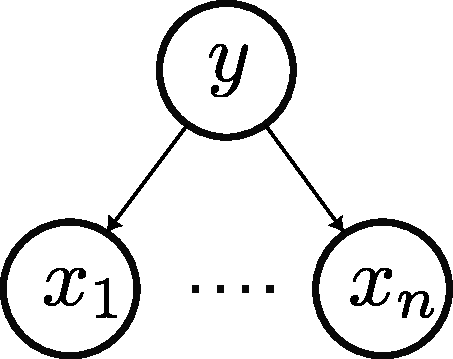
\includegraphics[scale=0.5]{./images/conditional_independence.pdf}
		\end{figure}
    \item This allows us to write the class conditional density as a product of one dimensional densities:
    $$p(\mathbf{x}|y=c, \boldsymbol{\theta}) = \prod_{j=1}^{D}p(x_j|y=c,\boldsymbol{\theta}_{jc})$$
  \end{itemize}
  The resulting model is called a \textbf{naive Bayes classifier (NBC)}. The model is called ``naive'' since we assume the independence between the features, which is not true in practice. However, if often results in classifiers that work well.

  The form of the class-conditional density depends on the type of each feature. We give some possibilities below:
  \begin{itemize}
    \item In the case of real-valued features, we can use the Gaussian distribution: $p(\mathbf{x}|y=c, \boldsymbol{\theta}) = \prod_{j=1}^{D}\mathcal{N}(x_j|\mu_{jc}^2)$, where $\mu_{jc}$ is the mean of feature $j$ in objects of class $c$, and $\sigma_{jc}^2$ is its variance.
    \item In the case of binary features, we can use the Bernoulli distribution: $p(\mathbf{x}|y=c, \boldsymbol{\theta}) = \prod_{j=1}^{D}\textrm{Ber}(x_j|\mu_{jc})$, where $\mu_{jc}$ is the probability that feature $j$ occurs in class $c$. This is sometimes called the \textbf{multivariate Bernoulli naive Bayes} model.
    \item In the case of categorical features, $x_j\in \{1,...,K\}$, we can model the multinomial distribution: $p(\mathbf{x}|y=c, \boldsymbol{\theta}) = \prod_{j=1}^{D}\textrm{Cat}(x_j|\mu_{jc})$, where $\boldsymbol{\mu}_{jc}$ is a histogram over the $K$ possible values for $x_j$ in class $c$.
  \end{itemize}

The probability for a single data case is given by
$$p(\mathbf{x}_i,y_i|\boldsymbol{\theta}) = p(y_i|\boldsymbol{\pi})\prod_{j}p(x_{ij}|\boldsymbol{\theta}_j)=\prod_{c}\pi_{c}^{\mathds{I}(y_i=c)}\prod_{j}\prod_{c}p(x_{ij}|\boldsymbol{\theta}_{jc})^{\mathds{I}(y_i=c)},$$
where $\boldsymbol{\pi}$ is a vector of class probability. Hence the log-likelihood is given by
	$$\textrm{log}p(\mathcal{D}|\boldsymbol{\theta}) = \sum_{c=1}^{C}N_c\textrm{log}\pi_c+\sum_{j=1}^{D}\sum_{c=1}^{C}\sum_{i:y_i=c}\textrm{log}p(x_{ij}|\boldsymbol{\theta}_{jc})$$

	\begin{algorithm}[H]
		\SetAlgoLined
%		\KwResult{Write here the result }
		Initialize $N_c=0,N_{jc}=0$ \;
		\For{$i=1:N$}{
      $c=y_i$ //Class label of $i$-th example;

      $N_c:=N_c+1$;

  		\For{$j=1:D$}{
      \uIf{$x_{ij}=1$}{
        $N_{jc}:=N_{jc}+1$
        }
  		}
		}
  $\hat{\pi}=\frac{N_c}{N},\hat{\theta}_{jc}=\frac{N_{jc}}{N_c}$
	\caption{Fitting a naive Bayes classifier to binary features}
\end{algorithm}

\section{Logistic Regression}
\label{sec:logistic_regression}

Logistic regression corresponds to the following binary classification model:
$$p(y|\mathbf{x},\mathbf{w})=\textrm{Ber}(y|\sigma(\mathbf{w}^T\mathbf{x}))$$

Logistic regression modles a logit (log odds) through a linear model. For binary data, the goal is to model the probability $p$ that one of two outcomes occurs. The logit function is $\textrm{log}\frac{p}{1-p}$, which varies between $-\infty$ and $+\infty$ as $p$ varies between $0$ and $1$.
$$\textrm{log}\frac{p}{1-p} = w_0x_0 +  w_1x_1 + ... + w_nx_n$$
Note that the logistic regression model assumes that the log-odds (\textit{logit}) of an observation $y$ can be expressed as a linear function. In this context, the logit function is called the \textbf{\textit{link function}} because it ``links'' the probability to the linear function of the predictor variables.

% Simplest solution to model a dependant variable $y$ is a linear regression. However, $y$ should be in a range of $[0,1]$. So we need to introduce the logit function. 

% The linear regression can be generalized to the classification setting with two changes:
% \begin{itemize}
% 	\item Replacing the Gaussian distribution for $y$ with a Bernoulli distribution: $p(y|\mathbf{x},\mathbf{w})=Ber(y|\mu(\mathbf{x}))$
% 	\item Squashing input data into sigmoid function $\sigma(\eta)$ that range from 0 to 1: $\sigma(\eta)\triangleq \frac{1}{1+exp(-\eta)}$.
% \end{itemize}
% $$p(y|\mathbf{x},\mathbf{w})=Ber(y|\sigma(\mathbf{w}^T\mathbf{x})),\$$

The negative log-likelihood for logistic regression is given by
\begin{align*}
	\textrm{NLL}(\mathbf{w}) &= -\sum_{i=1}^{N}\textrm{log}[\mu_i^{\mathds{I}(y_i=1)}\times (1-\mu_i)^{\mathds{I}(y_i=0)}]\\
	&=-\sum_{i=1}^{N}[y_i\textrm{log}\mu_i + (1-y_i) \textrm{log}(1-\mu_i)], \textrm{ }\footnotemark
\end{align*}
where $\mu=\sigma(\mathbf{w}^T\mathbf{x})$. This is also called \textbf{cross-entropy} error function. 
\footnotetext{$\mathds{I}(y_i=1) = y_i$, because $y_i\in \{0, 1\}$ is a binary variable}

Another way to express \textrm{NLL} is as follows. Suppose $\hat{y}_i\in\{-1,+1\}$ instead of $y_i\in\{0,1\}$. We have $p(y=1)=\frac{1}{1+\mathrm{exp}(-\mathbf{w}^T\mathbf{x})}$ and $p(y=-1)=\frac{1}{1+\mathrm{exp}(+\mathbf{w}^T\mathbf{x})}$. Hence
\begin{align*}
	\textrm{NLL}(\mathbf{w}) &= -\frac{1}{N}\sum_{n=1}^N [\mathbb{I}(\hat{y}_n=1)\log(\sigma(a_n))+\mathbb{I}(\hat{y}_n=-1)\log(\sigma(-a_n))]\\
							 &= -\frac{1}{N}\sum_{n=1}^N \log(\sigma(\hat{y}_na_n))\\
							 &=  \frac{1}{N}\sum_{i=1}^{N}\textrm{log}(1+\mathrm{exp}(-\hat{y}_i\mathbf{w}^T\mathbf{x}_i).
\end{align*}
Note that the sigmoid is used for compressing the output into $[0,1]$ and $\sigma(-a_n) = 1-\sigma(a_n)$. Unlike the linear regression, there is no closed from solution for logistic regression, thus we need optimization algorithms for it. Typically, optimization process involves the gradient and Hessian. 
\begin{align*}
	\mathbf{g}&=\frac{d}{d\mathbf{w}}\mathrm{NLL}(\mathbf{w})=\frac{d}{d\mu_i}\mathrm{NLL}(\mathbf{w})\frac{d\mu_i}{d\mathbf{h}}\frac{d\mathbf{h}}{d\mathbf{w}}\\
	& = \sum_{i=1}\Bigg[-\frac{y_i}{\mu_i} + \frac{(1-y_i) }{(1-\mu_i)}\Bigg]\frac{d\mu_i}{d\mathbf{h}}\frac{d\mathbf{h}}{d\mathbf{w}}=\sum_{i=1}\Bigg[\frac{\mu_i-y_i }{\mu_i(1-\mu_i)}\Bigg]\frac{d\mu_i}{d\mathbf{h}}\frac{d\mathbf{h}}{d\mathbf{w}}\\
	&=\sum_{i}(\mu_i-y_i)\mathbf{x}_i=\mathbf{X}^T(\boldsymbol{\mu}-\mathbf{y})\\
	\frac{d\mu_i}{d\mathbf{h}}& = \mu_i(1-\mu_i)\\
	\frac{d\mathbf{h}}{d\mathbf{w}}& = \mathbf{x}_i
\end{align*}
where $\mathbf{h}=\mathbf{w}^T\mathbf{x}$. 

We can also use the second-order method. 
\begin{align*}
\mathbf{H}&=\frac{d}{d\mathbf{w}}g(\mathbf{w})^T=\sum_{i}(\nabla_{\mathbf{w}}\mu_i)\mathbf{x}_i^T=\sum_{i}\mu_i(1-\mu_i)\mathbf{x}_i\mathbf{x}_i^T\\
&=\mathbf{X}^T\mathbf{S}\mathbf{X},
\end{align*}
where $\mathbf{S}\triangleq \mathrm{diag}(\mu_i(1-\mu_i))$. Note that $\mathbf{H}$ is positive definite, because the \textrm{NLL} is convex and has a global minimum. 




\chapter{Bayesian Regression}

Integrate over all $\theta$

\begin{align}
P(heads \mid D) =& \int_{\theta} P(heads, \theta \mid D) d\theta\\
 =& \int_{\theta} P(heads \mid \theta, D) P(\theta \mid D) d\theta \ \ \ \ \ \  \textrm{(Chain rule: $P(A,B|C)=P(A|B,C)P(B|C)$.)}\\ 
  =& \int_{\theta} \theta P(\theta \mid D) d\theta\\ 
  =&E\left[\theta|D\right]\\
 =&\frac{n_H + \alpha}{n_H + \alpha + n_T + \beta}
\end{align}


% \chapter{Introduction}
\section{Curve Fitting}
We can assume that a target variable has a Gaussian distribution with a mean equal to the value $y(x,\mathbf{w})$ of the polynomial curven given by
\begin{equation}
	p(t|x, \mathbf{w}, \beta) = \mathcal{N}(t|y(x,\mathbf{w}), \beta^{-1}),
	\label{eq:curve}
\end{equation}
\begin{itemize}
	\item $t$: target variable
		$$t = y(\rvx, \rvw) +\epsilon,$$
	where $\epsilon$ is a zero mean Gaussian noise with precision (inverse variance) $\beta$. 
	% \item $x$: input
	% \item $\beta$: an inverse variance of the distribution.
\end{itemize}

We not use the training data $\{\mathbf{x,y}\}$ to determine the values of the unknown parameters $\mathbf{w}$ and $\beta$ by maximum likelihood. If the data are assumed to be drawn independently from the distribution, then the likelihood function is given by 
\begin{equation}
	p(\mathbf{t}|\mathbf{x,w},\beta) = \prod_{n=1}^{N}\mathcal{N}(t_n|y(x_n,\mathbf{w}), \beta^{-1}).
	\label{eq:curve_ml}
\end{equation}

We can take a step towards a more Bayesian approach and introduce a prior distribution over the polynomial coefficients $\mathbf{w}$. For simplicity, we can use a Gaussian distribution from
\begin{equation}
	p(\mathbf{w}|\alpha) = \mathcal{N}(\mathbf{w|0},\alpha^{-1}\mathbf{I}),
	\label{eq:prior_hyper}
\end{equation}
where $\alpha$ is the precision of the distribution. Using Bayes' theorem, the posterior distribution for $\mathbf{w}$ is proportional to the product of the prior distribution and the likelihood function
\begin{equation}
	p(\mathbf{w|x,t},\alpha,\beta)\propto p(\mathbf{w|x,t},\beta)p(\mathbf{w},\alpha).
	\label{eq:bayes_reg}
\end{equation}
We can now determined $\mathbf{w}$ by finding the most probable value of $\mathbf{w}$ given the data, in other words by maximizing the posterior distribution, MAP (maximum posterior). Taking a negative logarithm, then we can find that the maximum of the posterior is given by the minimum of 
\begin{equation}
	\frac{\beta}{2}\sum_{n=1}^N \{y(x_n,\mathbf{w})-t_n\}^2+\frac{\alpha}{2}\mathbf{w}^T\mathbf{w}.
	\label{eq:bayes_}
\end{equation}
Thus we see that maximizing the posteiror distribution si equivalent to minimizing the regularized sum of squares error function encountered earler with a regularization parameter given by $\lambda = \alpha/\beta$.



\section{Bayesian Curve Fitting}


% \section{Adding Noise to Regression Predictors is Ridge Regression}
% In linear regression, we seek a vector $\hat{\beta}$ which solves the following optimization problem:
% \begin{equation}
% 	\hat{\beta} = \arg\min_{\beta}|y-X\beta|^2
% 	\label{eq:linear_regression}
% \end{equation}

% Ridge regression is

% \begin{equation}
% 	\hat{\beta} = \arg\min_{\beta}|y-X\beta|^2+\lambda|\beta|^2
% 	\label{eq:ridge_linear_regression}
% \end{equation}

% $$\varepsilon_1,\varepsilon_2,\cdots\sim \mathcal{N}(1,\sigma),$$
% We can add a multiplicitive random noise to $\mathbf{X}$.
% $$x_{ij}\to \varepsilon_{ij}x_{ij}$$

% $$\hat{\beta} \sim \arg\min_{\beta} E_{G}[|y-G\cdot X\beta|^2]$$
% where $G$ is a matrix of random Gaussian noise. 

% \begin{align*}
% 	\mathbb{E} \left[ \left| y - (G * X) \beta  \right|^2 \right] &= E \left[ y^t y - 2 y^t (G * X) \beta + \beta^t (G * X)^t (G * X) \right] \\
% &= y^t y - 2 y^t (E[G] * X) \beta + \beta^t E \left[ M \right] \beta \\
% &= y^t y - 2 y^t X \beta + \beta^t X^t X \beta + \beta^t diag(\sigma^2) X^t X \beta \\
% &= \left| y - X \beta \right|^2 + \beta^t diag(\sigma^2) X^t X \beta \\
% &= \left| y - X \beta \right|^2 + \sigma^2 \left| \Gamma \beta \right|^2
% \end{align*}
% where $M = (G\cdot X)^T(G\cdot X)$
% $$m_{ij} = \sum_k e_{ki}e_{kj}x_{ki}x_{kj}$$

	

\chapter{Training, Testing, and Regularization}
\section{Sources of Error in ML}
$$E_{out} \leq E_{ml}+\Omega$$
\begin{itemize}
	\item $E_{out}$: estimation of error. 
	\item $E_{ml}$: error from a learning algorithm
	\item $\Omega$: error caused by the variance from observations. 
\end{itemize}
We also define 
\begin{itemize}
	\item $f$: target function
	\item $g$: learning function
	\item $g^{(D)}$: learned function based on $D$, or simply \textit{hypothesis}.
	\item $D$: dataset drawn from the real world.
	\item $\bar{g}$: the average hypothesis of a given infinite number of $D$s. 
		$$\bar{g}(x) = \mathbb{E}_D[g^{(D)}(x)].$$
\end{itemize}

Error of a single instance $x$ from $g$ learnt from $D$ is given by
\begin{align*}
	Err_{\textrm{out}}(g^{(D)}(x)) = \mathbb{E}_{X}[(g^{(D)}(x)-f(x))^2],
\end{align*}
where $X$ can be considered as test sets. Then, the expected error over the infinite number of datasets $D$ sampled from a true data distribution is
\begin{align*}
	\mathbb{E}_D[Err_{\textrm{out}}(g^{(D)}(x))] &= \mathbb{E}_D[\mathbb{E}_{X}[(g^{(D)}(x)-f(x))^2]]\\
												 &= \mathbb{E}_X[\mathbb{E}_D[(g^{(D)}(x)-f(x))^2]]
\end{align*}
Let's simplify the term inside with an average of hypothesis $\bar{g}(x)$:
\begin{align*}
	\mathbb{E}_D[(g^{(D)}(x)-f(x))^2]&= \mathbb{E}_D[(g^{(D)}(x)-\bar{g}(x)+\bar{g}(x)-f(x))^2]\\
	&= \mathbb{E}_D\big[(g^{(D)}(x)-\bar{g}(x))^2+(\bar{g}(x)-f(x))^2\\ &\quad + 2 (g^{(D)}(x)-\bar{g}(x))(\bar{g}(x)-f(x))\big]\\
	&= \mathbb{E}_D\big[(g^{(D)}(x)-\bar{g}(x))^2\big]+(\bar{g}(x)-f(x))^2\\ &\quad + \mathbb{E}_D\big[2 (g^{(D)}(x)-\bar{g}(x))(\bar{g}(x)-f(x))\big]
\end{align*}
Since, $\mathbb{E}_D\big[2 (g^{(D)}(x)-\bar{g}(x))(\bar{g}(x)-f(x))\big]$ is 0, the expectation of the error becomes
\begin{align*}
	\mathbb{E}_D[Err_{\textrm{out}}(g^{(D)}(x))] = \mathbb{E}_X\big[\mathbb{E}_D\big[(g^{(D)}(x)-\bar{g}(x))^2\big]+(\bar{g}(x)-f(x))^2\big].
\end{align*}
Let's closely look at this formula. The errors are from two sources:
\begin{itemize}
	\item \textbf{Variance}: $\mathbb{E}_D\big[(g^{(D)}(x)-\bar{g}(x))^2\big]$. Variance captures how much your classifier changes if you train on a different training set. We need to collect more data to reduce the variance. 
	\item \textbf{Bias}: $(\bar{g}(x)-f(x))^2$. Bias is the inherent error that you obtain from your classifier even with infinite training data. We need to build a more complex model to reduce the bias. 
\end{itemize}
However, if we reduce the bias, then the variance tends to increase. 

\subsection{Alternative Derivation}

The derivation of the bias–variance decomposition for squared error proceeds as follows.[6][7] For notational convenience, abbreviate $f = f(x)$ and $\hat{f} = \hat{f}(x)$. First, recall that, by definition, for any random variable $\mathbf{X}$, we have
$$\displaystyle \operatorname {Var} {\big [}{\hat {f}}(x){\big ]}=\operatorname {E} [X^{2}]-\operatorname {E} [X]^{2}.$$
By rearranging, we get 
$$\operatorname {E} [X^{2}] = \displaystyle \operatorname {Var} {\big [}{\hat {f}}(x){\big ]}+\operatorname {E} [X]^{2}.$$
Since $f$ is deterministic
$$\operatorname {E} [f] = f$$

Thus, given $y = f+\varepsilon$ and $\operatorname {E} [\varepsilon] = 0$, implies $\operatorname {E} [y] = \operatorname {E} [f+\varepsilon] = \operatorname {E} [f] = f$

Also, since $\operatorname{Var} [\varepsilon ]=\sigma ^{2}$
$$\displaystyle \operatorname {Var} [y]=\operatorname {E} [(y-\operatorname {E} [y])^{2}]=\operatorname {E} [(y-f)^{2}]=\operatorname {E} [(f+\varepsilon -f)^{2}]=\operatorname {E} [\varepsilon ^{2}]=\operatorname {Var} [\varepsilon ]+{\Big (}\operatorname {E} [\varepsilon ]{\Big )}^{2}=\sigma ^{2}$$

Thus, since $\varepsilon$ and $\hat {f}$ are independent, we can write:
\begin{align*}
	\operatorname {E} {\big [}(y-{\hat {f}})^{2}{\big ]}&=\operatorname {E} {\big [}(f+\varepsilon -{\hat {f}})^{2}{\big ]}\\
	&=\operatorname {E} {\big [}(f+\varepsilon -{\hat {f}}+\operatorname {E} [{\hat {f}}]-\operatorname {E} [{\hat {f}}])^{2}{\big ]}\\
	&=\operatorname {E} {\big [}(f-\operatorname {E} [{\hat {f}}])^{2}{\big ]}+\operatorname {E} [\varepsilon ^{2}]+\operatorname {E} {\big [}(\operatorname {E} [{\hat {f}}]-{\hat {f}})^{2}{\big ]}+2\operatorname {E} {\big [}(f-\operatorname {E} [{\hat {f}}])\varepsilon {\big ]}+\\
	&\quad 2\operatorname {E} {\big [}\varepsilon (\operatorname {E} [{\hat {f}}]-{\hat {f}}){\big ]}+2\operatorname {E} {\big [}(\operatorname {E} [{\hat {f}}]-{\hat {f}})(f-\operatorname {E} [{\hat {f}}]){\big ]}\\
	&=(f-\operatorname {E} [{\hat {f}}])^{2}+\operatorname {E} [\varepsilon ^{2}]+\operatorname {E} {\big [}(\operatorname {E} [{\hat {f}}]-{\hat {f}})^{2}{\big ]}+\\
	&\quad 2(f-\operatorname {E} [{\hat {f}}])\operatorname {E} [\varepsilon ]+2\operatorname {E} [\varepsilon ]\operatorname {E} {\big [}\operatorname {E} [{\hat {f}}]-{\hat {f}}{\big ]}+2\operatorname {E} {\big [}\operatorname {E} [{\hat {f}}]-{\hat {f}}{\big ]}(f-\operatorname {E} [{\hat {f}}])\\
	&=(f-\operatorname {E} [{\hat {f}}])^{2}+\operatorname {E} [\varepsilon ^{2}]+\operatorname {E} {\big [}(\operatorname {E} [{\hat {f}}]-{\hat {f}})^{2}{\big ]}\\
	&=(f-\operatorname {E} [{\hat {f}}])^{2}+\operatorname {Var} [y]+\operatorname {Var} {\big [}{\hat {f}}{\big ]}\\
	&=\operatorname {Bias} [{\hat {f}}]^{2}+\operatorname {Var} [y]+\operatorname {Var} {\big [}{\hat {f}}{\big ]}\\
	&=\operatorname {Bias} [{\hat {f}}]^{2}+\sigma ^{2}+\operatorname {Var} {\big [}{\hat {f}}{\big ]}
\end{align*}

\part{Kernel Methods}
\chapter{Kernel Methods}
\begin{itemize}
	\item The main idea is to use large set of fixed non-linear basis functions.
	\item The complexity depends on number of basis functions, but dual trick changes it to a size of dataset. 
\end{itemize}

Kernel function: Let $\phi(\rvx)$ be a set of basis functions that map inputs $\rvx$ to a feature space. In many algorithms, this feature space only appears in a dot product $\phi(\rvx)^T\phi(\rvx')$ of input pairs $\rvx$ and $\rvx'$. Then, kernel function can be defined as $k(\rvx, \rvx') = \phi(\rvx)^T\phi(\rvx')$. Note that we only need to know $k(\rvx, \rvx')$, not $\phi(\rvx)$.
\begin{itemize}
	\item The kernel function is a measure of similarity between $\rvx_i$and $\rvx_j$ 
\end{itemize}

A function $k: \mathbb{R}^d\times \mathbb{R}^d\to \mathbb{R}$ is said to be a positive semidefinite kernel if it is symmetric, (\ie $k(\rvx',\rvx)= k(\rvx,\rvx')$).

Recall that the linear regression can be modelee as follows:
$$f(\rvx) = \rvx^T\rvw,$$
where $\rvx = [x_1, \dots, x_m]^T$ and $\rvw = [w_1,\dots,w_m]$. The ridge regression for $\mathbf{X}\in \mathbb{R}^{n\times m}$ matrix can be modeled as follows:
\begin{align}
	J(\rvw) &= \|\mathbf{y}-\mathbf{X}\rvw\|^2_2 + \lambda \|\rvw\|^2_2 \\
			&= (\mathbf{y}-\mathbf{X}\rvw)^T(\mathbf{y}-\mathbf{X}\rvw)+\lambda\rvw^T\rvw\\
			&= (\mathbf{y}^T-\rvw^T\mathbf{X}^T)(\mathbf{y}-\mathbf{X}\rvw)+\lambda\rvw^T\rvw\\
			&= \rvy^T\rvy-\rvw^T\mathbf{X}^T\rvy-\rvy^T\mathbf{X}\rvw+\rvw^T\mathbf{X}^T\mathbf{X}\rvw+\rvw^T\lambda\mathbf{I}\rvw\\
	\frac{\partial J}{\partial \rvw}&= -\mathbf{X}^T\rvy-\mathbf{X}^T\rvy+\mathbf{X}^T\mathbf{X}\rvw+\mathbf{X}^T\mathbf{X}\rvw+2\lambda\mathbf{I}\rvw = 0\\
	\rvw	&= (\mathbf{X}^T\mathbf{X}+\lambda\mathbf{I})^{-1}\mathbf{X}^T\rvy
	\label{eq:ridge_regression}
\end{align}
Let's change it into a dual form:
\begin{align}
	(\mathbf{X}^T\mathbf{X}+\lambda\mathbf{I})\rvw	&= (\mathbf{X}^T\mathbf{X}+\lambda\mathbf{I})(\mathbf{X}^T\mathbf{X}+\lambda\mathbf{I})^{-1}\mathbf{X}^T\rvy\\
	(\mathbf{X}^T\mathbf{X}+\lambda\mathbf{I})\rvw &= \mathbf{X}^T\rvy\\ 
	\rvw &= \lambda^{-1}\mathbf{I}(\mathbf{X}^T\rvy-\mathbf{X}^T\mathbf{X}\rvw)\\
	&= \mathbf{X}^T\lambda^{-1}(\rvy-\mathbf{X}\rvw)\\
	&= \mathbf{X}^T\alpha\\
	\lambda\alpha &= (\rvy-\mathbf{X}\rvw)\\
	&= (\rvy-\mathbf{X}\mathbf{X}^T\alpha)\\
	\rvy &= (\mathbf{X}\mathbf{X}^T\alpha+\lambda\alpha)\\
	\alpha &= (\mathbf{X}\mathbf{X}^T+\lambda)^{-1}\rvy\\
	\alpha &= (\mathbf{G}+\lambda)^{-1}\rvy,
	\label{eq:dual_regression}
\end{align}
where $\mathbf{G} = \mathbf{X}\mathbf{X}^T$ is a \textit{Gram matrix}. Thus, we just have to solve $m\times m$ matrix. 

Therefore, given a new input $\rvx'\in \mathbb{R}^m$, the prediction $f(\rvx') = (\rvx')^T\rvw $ can be expressed as follows:
$$f(\rvx') = (\rvx')^T\mathbf{X}^T(\mathbf{X}\mathbf{X}^T+\lambda\mathbf{I})^{-1}\rvy.$$

Note that this formula depends only on the data via inner products. 
\begin{align*}
	(\rvx')^T\mathbf{X}^T = 
	\begin{bmatrix}
		\langle \rvx',\rvx_1\rangle\\
		\vdots\\
		\langle \rvx',\rvx_n\rangle
	\end{bmatrix}^T,\quad
	\mathbf{X}\mathbf{X}^T = 
	\begin{bmatrix}
		\langle \rvx_1,\rvx_1\rangle& \dots& \langle \rvx_1,\rvx_n\rangle\\
		\vdots&\ddots&\vdots\\
		\langle \rvx_n,\rvx_1\rangle &\dots &\langle \rvx_n,\rvx_n\rangle
	\end{bmatrix}
\end{align*}
Therefore, we can apply the kernel trick and consider the more general prediction function.


% Then, the closed-form solution of the ridge regression is given by
% $$\hat{\boldsymbol{\theta}} = (\mathbf{X}^T\mathbf{X}+\lambda\mathbf{I})^{-1}\mathbf{X}^T\mathbf{y}.$$


% We can rewrite it by $\rvw = \Phi \rva$, where $\Phi = [\phi(\rvx_1),\dots,\phi(\rvx_N)]$, $\rva = [a_1,\dots,a_N]^T$, and $a_n =-\frac{1}{\lambda} (\rvw^T\phi(\rvx_n)-y_n).$. Then, we get a dual objective, which aims to minimize $E$ with respect to $\rva$.

% Let $K = \Phi^T\Phi$ be the Gram matrix. 


\section{Gaussian Process}
\label{sec:gaussian_process}
Gaussian processes are distributions over functions $f(x)$ of which the distribution is defined by a mean function $m(x)$ and positive definite covariance function $k(x,x')$:
$$f(x) \sim \mathcal{GP}(m(x),k(x,x')).$$

Let $f(x) = \phi(x)^Tw$, with $w\sim \mathcal{N}(0, \alpha^{-1}\mathbf{I})$. Then, $m(x) = \mathbb{E}[f(x)] = \mathbb{E}[w]^T\phi(x) = 0$

$k(x, x') = \mathbb{E}[(f(x)-m(x))(f(x')-m(x'))] =\mathbb{E}[f(x)(f(x')] $


\chapter{Support Vector Machine}
\section{Introduction}

\subsection{Orthogonal Projection}
Given two vectors $x$ and $y$, we would like to find the orthogonal projection of $x$ onto $y$.

By definition:
$$||z|| = ||x||cos(\theta).$$
Note that the dot product of $x$ and $y$ is 
$$cos(\theta)= \frac{x\cdot y}{||x||\cdot||y||}.$$
So we can replace the cosine 
$$||z|| = ||x||\frac{x\cdot y}{||x||\cdot||y||}.$$
This results in 
$$||z|| = u\cdot x,$$
where $u$ is an unit vector of $y$, which has the same direction as $z$. Therefore we can express $z$ as follows: 
$$z = ||z||\cdot u,$$
Then, 
\begin{align*}
	z &= (u\cdot x)u.
\end{align*}
Equivalently, 
\begin{align*}
	\textrm{Proj}_yx &= \Bigg(\frac{y\cdot x}{||y||^2}\Bigg)y.
\end{align*}

\section{Decision Boundary with Margin}

Support vectors are the data points that lie closest to the decision surface(or hyperplane). They are directly related to the optimal hyperplane. The goal of SVM is to find the optimal separating hyperplane which maximizes the margin of the training data. The hyperplane can be written as the set of points $\mathbf{x}$, satisfying 
$$\mathbf{w}\cdot \mathbf{x}+b=0$$
Note that the hyperplain is normal to the vector $\mathbf{w}$. 
$$\mathbf{w}(\mathbf{x}-\mathbf{x}_0)=0,$$
where $b = \mathbf{w}\cdot\mathbf{x}_0$. However, what is the optimal separating hyperplanes? The optimal hyperplane is the one which maximizes the margin of the training data. SVMs maximize the margin around the separating hyperplane. The decision function is fully specified by a subset of training samples, the support vectors. Let's consider a simple case, where training data is linearly separable, $\mathcal{D} = \left\{ (\mathbf{x}_i, y_i)\mid\mathbf{x}_i \in \mathbb{R}^p,\, y_i \in \{-1,1\}\right\}_{i=1}^n$. Then, we can build two hyperplanes separating the data with no points between them:
\begin{itemize}
	\item $H_1:\mathbf{w}\cdot \mathbf{x}+b=1$
	\item $H_2:\mathbf{w}\cdot \mathbf{x}+b=-1$
\end{itemize}

There are two constraints:
\begin{enumerate}
	\item $\mathbf{w}\cdot \mathbf{x}+b\geq1$
	\item $\mathbf{w}\cdot \mathbf{x}+b\leq-1$
\end{enumerate}
These can be combined as follows:
$$y(\mathbf{w}\cdot \mathbf{x}+b)\geq 1.$$

To maximize the margin, we can consider a unit vector $\mathbf{u} = \frac{\mathbf{w}}{||\mathbf{w}||}$, which is perpendicular to the hyperplanes and a point $x_0$ on the hyperplane $H_2$. If we scale $u$ from $x_0$, we get $z = x_0+ru$. If we assume $z$ is on $H_1$, then $\mathbf{w}\cdot z +b=1$. This is equivalent to 
\begin{align*}
	\mathbf{w}\cdot (x_0+ru)+b=1\\
	\mathbf{w}x_0+\mathbf{w}r\frac{\mathbf{w}}{||\mathbf{w}||}+b=1\\
	\mathbf{w}x_0+r||\mathbf{w}||+b=1\\
	\mathbf{w}x_0+b=1-r||\mathbf{w}||
\end{align*}
$x_0$ is on $H_2$, so $\mathbf{w}x_0+b=-1$
\begin{align*}
	-1=1-r||\mathbf{w}||\\
	r=\frac{2}{||\mathbf{w}||}
\end{align*}
Note that the scaled unit vector $ru$'s magnitude is $r$. Thus, the maximization of margin is equivalent to maximize $r$. To maximize $r$, it is important to minimize the norm of $\mathbf{w}$. This is equivalent to an optimization problem. 
\begin{align*}
	&\min ||w||,\quad \textrm{subject to } \\
	&y_i(\mathbf{w}\cdot \mathbf{x}_i+b)\geq 1 \quad\forall i.
\end{align*}
This minimization problem gives the same result as the following:  
\begin{align*}
	&\min \frac{1}{2}||w||^2,\quad \textrm{subject to } \\
	&y_i(\mathbf{w}\cdot \mathbf{x}_i+b)\geq 1 \quad\forall i.
\end{align*}
Now, we now have \textbf{convex quadratic optimization problem}. However, this hard margin cannot tolerate erroneous cases. There could be two solutions:
\begin{itemize}
	\item Admits prediction errors. 
	\item Use non-linearity (complex decision boundary).
\end{itemize}

\section{Error Handling in SVM}
Let's first try to solve the issue by allowing some prediction errors. 
\begin{align*}
	&\min ||w||+C\cdot N_{e},\quad \textrm{subject to } \\
	&y_i(\mathbf{w}\cdot \mathbf{x}_i+b)\geq 1 \quad \forall i.
\end{align*}
where $N_e$ is the number of errors. It means we consider all errors equally. This penalty approach is \textbf{0-1 loss}. This approach is not popular, since it is hard to solve. Another approach is to use a \textbf{slack variable} with \textbf{hinge loss}, instead of counting the number of errors. 
\begin{align*}
	&\min ||w||+C\sum_j\xi_j ,\quad \textrm{subject to } \\
	&y_i(\mathbf{w}\cdot \mathbf{x}_i+b)\geq 1-\xi_j \quad \forall i,\, \xi_j\geq 0,\, \forall j.
\end{align*}
Note that $\xi_j>1$ when mis-classified by its definition: 
\begin{align*}
	\xi_j = (1-(\mathbf{w}x_j+b)y_j)_+
\end{align*}
Let's look at the new constraint. If some data points are mis-classified, then $\xi_j>1$ and $y_i(\mathbf{w}\cdot \mathbf{x}_i+b)\leq 0$. This approach is called \textbf{soft-margin SVM}. Lastly, how do we set $C$?

\section{Kernel Trick}
\label{sec:kernel_trick}
Applying the kernel trick simply means replacing the dot product of two examples in a dual form by a kernel function. 

\begin{align}
	 \max_\alpha \sum_i \alpha_i -\frac{1}{2}\sum_i\sum_j \alpha_i\alpha_j y_iy_j \psi(\mathbf{x}_i)\cdot \psi(\mathbf{x}_j)
	 \label{eq:kernel_dual_form}
\end{align}
Equivalently, 
\begin{align}
	 \max_\alpha \sum_i \alpha_i -\frac{1}{2}\sum_i\sum_j \alpha_i\alpha_j y_iy_j K(\mathbf{x}_i,\mathbf{x}_j)
\end{align}














\section{SVM Optimization: Lagrange Multipliers}

\begin{align*}
&\min_{\rvx} f(\rvx) \\
&\textrm{subject to}\quad g(\rvx)=0.\\
\end{align*}
The minimum of $f$ is found when its gradient point in the same direction as the gradient of $g$. In other words, when:  
$$\nabla f(\rvx) = \alpha\nabla g(\rvx)$$
So if we want to find the minimum of $f$ under the constraint $g$, we just need to solve the following function: 
$$\mathcal{L}(\rvx, \alpha) = f(\rvx) - \alpha g(\rvx)$$
Note that the $\alpha$ is called a \textit{Lagrange multiplier}. 

Recall that we want to solve the following convex quadratic optimization problem:
\begin{align*}
	&\min \frac{1}{2}||w||^2,\quad \textrm{subject to } \\
	&y_i(\mathbf{w}\cdot \mathbf{x}_i+b)\geq 1 \quad\forall i.
\end{align*}
We can reformulate the above problem as follows:
\begin{align}
	\mathcal{L}(\rvw, b, \alpha) = \frac{1}{2}||w||^2 - \sum_i \alpha_i \Big[y_i(\mathbf{w}\cdot \mathbf{x}_i+b)-1\Big]
	\label{eq:objective_function}
\end{align}
We could try to solve the optimization problem, but this problem can only be solved analytically when the number of examples is small. Thus, we will reformulate the problem in the duality principle. 

To get the solution of the primal problem, we need to solve the following \textbf{Lagrangian problem}: 
\begin{align*}
	&\max_{\mathbf{w}, b}\min_\alpha \mathcal{L}(\rvw, b, \alpha)\\
	&\textrm{subject to}\quad \alpha_i\geq 0, \forall i.\\
\end{align*}

You may have noticed that the method of Lagrange multipliers is used for solving problems with equality constraints, and here we are using them with inequality constraints. This is because the method still works for inequality constraints, provided some additional conditions (the \textbf{KKT conditions}) are met. We will discuss about this soon.

\section{The Wolfe Dual Problem}
The Lagrangian problem has $m$ inequality constraints (where $m$ is the number of training examples) and is typically solved using its \textit{dual form}. The duality principle tells us that \textbf{an optimization problem can be viewed from two perspectives}: \Ni The first one is the \textit{primal problem}, a minimization problem in our case. \Nii The other one is the \textit{dual problem}, which will be a maximization problem. What is interesting is that the maximum of the dual problem will always be less than or equal to the minimum of the primal problem (we say it \textbf{provides a lower bound to the solution of the primal problem}). 

In our case, we are trying to solve a convex optimization problem, and \textbf{Slater's condition} holds for affine constraints (Gretton, 2016), so Slater’s theorem tells us that strong duality holds. Note that the strong duality denotes that the solutions from the dual and the primal are identical (the maximum of the dual problem is equal to the minimum of the primal problem). 

Solving the minimization problem involves taking the partial derivatives of $\mathcal{L}$ with respect to $\rvw$ and $b$.  
\begin{align*}
	&\nabla_\rvw\mathcal{L}(\rvw, b, \alpha) = \rvw - \sum_i \alpha_i y_i \mathbf{x}_i\\
	& \nabla_b\mathcal{L}(\rvw, b, \alpha) = -\sum_i \alpha_i y_i
\end{align*}
The first term gives
\begin{align*}
	&\rvw = \sum_{i=1}^m \alpha_i y_i \mathbf{x}_i\\
\end{align*}
Let's substitute the objective function \Cref{eq:objective_function} with $\rvw$:
\begin{align*}
	\mathbf{W}(\alpha, b) &= \frac{1}{2}\Big(\sum_i \alpha_i y_i \mathbf{x}_i\Big)\cdot \Big(\sum_j \alpha_j y_j \mathbf{x}_j\Big) - \sum_i \alpha_i \Bigg[y_i\Bigg(\Big(\sum_j \alpha_j y_j \mathbf{x}_j\Big)\cdot \mathbf{x}_i+b\Bigg)-1\Bigg]\\
						  &= \frac{1}{2}\Big(\sum_i\sum_j \alpha_i\alpha_j y_iy_j \mathbf{x}_i\cdot \mathbf{x}_j\Big) - \sum_i \alpha_i \Bigg[y_i\Bigg(\Big(\sum_j \alpha_j y_j \mathbf{x}_j\Big)\cdot \mathbf{x}_i+b\Bigg)\Bigg]+\sum_i \alpha_i \\
						  &= \frac{1}{2}\sum_i\sum_j \alpha_i\alpha_j y_iy_j \mathbf{x}_i\cdot \mathbf{x}_j - \sum_i\sum_j \alpha_i\alpha_j y_iy_j \mathbf{x}_i \cdot \mathbf{x}_j-\sum_i \alpha_i y_i b+\sum_i \alpha_i \\
						  &= \sum_i \alpha_i -\frac{1}{2}\sum_i\sum_j \alpha_i\alpha_j y_iy_j \mathbf{x}_i\cdot \mathbf{x}_j-\sum_i \alpha_i y_i b
\end{align*}
There is still $b$, but $b=0$, so we can just remove it. Finally, we get
\begin{align}
	 \mathbf{W}(\alpha, b) = \sum_i \alpha_i -\frac{1}{2}\sum_i\sum_j \alpha_i\alpha_j y_iy_j \mathbf{x}_i\cdot \mathbf{x}_j
	 \label{eq:dual_form}
\end{align}
This is the \textbf{Wolfe dual Lagrangian function}. Note that we transform the problem as a problem with regard to $\alpha$. Also, this is again a quadratic programming problem. The optimization problem is also called the \textbf{Wolfe dual problem}: 
\begin{align*}
	 &\max_\alpha \mathbf{W}(\alpha, b) = \sum_i \alpha_i -\frac{1}{2}\sum_i\sum_j \alpha_i\alpha_j y_iy_j \mathbf{x}_i\cdot \mathbf{x}_j\\
	 &\textrm{subject to } \alpha_i\geq 0 \textrm{ for any } i=1,\dots,m\\
	 & \sum_{i=1}^m \alpha_iy_i=0
\end{align*}
Once we get the value of $\alpha$, we can get the optimal $\rvw$ and $b$ can be obtained by using $\alpha_i(y_i(\mathbf{w}\cdot \mathbf{x}_i+b)-1=0$. Details will be covered in the following section.


\section{Karush-Kuhn-Tucker conditions }
Because we are dealing with inequality constraints, there is an additional requirement. The solution must also satisfy the \textbf{Karush-Kuhn-Tucker (KKT) conditions}. 

The KKT conditions are first-order necessary conditions for a solution of an optimization problem to be optimal. Moreover, the problem should satisfy some regularity conditions. Luckily for us, one of the regularity conditions is Slater’s condition, and we just saw that it holds for SVMs. Because the primal problem we are trying to solve is a convex problem, the KKT conditions are also sufficient for the point to be primal and dual optimal, and there is zero duality gap. 

To sum up, if a solution satisfies the KKT conditions, we are guaranteed that \textbf{it is the optimal solution}. Note that solving the SVM problem is equivalent to finding a solution to the KKT conditions. 





% \chapter{Explicit Generative Models}
Two important factors of explicit models to be determined:
\begin{itemize}
	\item Distributions
	\item Parameters of the distributions.
\end{itemize}

\part{Generative Modeling}
\chapter{Sampling Based Inference}
\section{Basic Sampling Methods}
% \subsection{Forward Sampling}

\subsection{Inverse Transform Sampling}
Inverse transform sampling is a basic method for pseudo-random number sampling, \ie for generating sample numbers at random from any probability distribution given its cumulative distribution function (CDF).

\textbf{Assume that we already have a uniformly distributed random number generator}, \eg \textrm{np.random.randn()}
\begin{enumerate}
	\item Generate a random number $u \sim Unif[0,1]$
	\item Find the inverse of the desired CDF, $F_{X}^{-1}(x)$.
	\item Compute $X=F_{X}^{-1}(u)$. The computed random variable $X$ has distribution $F_X(x)$
\end{enumerate}
However, it is \textbf{hard to compute the inverse of CDF} ($F_X(x)$)

	\begin{itemize}
		\item $F_X(x):\mathbb{R}\mapsto [0,1]$ is any CDF. 
		\item CDF is a non-negative and non-decreasing (monotone) function that is continuous. 
		\item Our objective is to simulate a random variable $X$ distributed as $F$; that is, we want to simularte a $X$ such that $P(X\leq x)=F(x)$.
		\item $F$ is invertible since it is continuous and strictly increasing.
%		\item $y$-axis: Uniform distribution
%		\item $x$-axis: sample value
	\end{itemize}

\begin{figure}[t]
	\begin{center}
		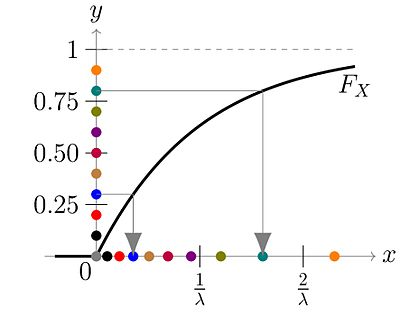
\includegraphics[scale=0.6]{./images/sampling/inverse.jpg}
	\end{center}
	\caption{$y$-axis: Uniform distribution, $x$-axis: sample value}
\end{figure}

\begin{figure}[t]
	\begin{center}
		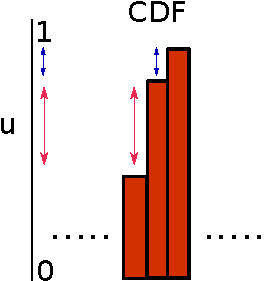
\includegraphics[scale=1.2]{./images/sampling/cdf.pdf}
	\end{center}
	\caption{How can this sampling method recover the original distribution?}
\end{figure}

\subsection{Ancestral Sampling}
$$p(\mathbf{x}) = p(\mathbf{x}_1)p(\mathbf{x}_2|\mathbf{x}_1)p(\mathbf{x}_3|\mathbf{x}_2)\cdots$$
Sampling steps:
\begin{enumerate}
	\item sample $\mathbf{x}_1$
	\item sample $\mathbf{x}_2$ conditioned by $\mathbf{x}_1$
	\item sample $\mathbf{x}_3$ conditioned by $\mathbf{x}_2$
\end{enumerate}



\subsection{Rejection Sampling}
Rejection sampling is a simple method. It rejects samples violating a given condition (\eg conditions of conditional probability.). Let's see its theory. 

Rejection sampling is a method for sampling from a distribution $p(x)=\frac{1}{Z}p'(x)$ that is difficulut to sample directly, but its unnormalized pdf $p'(x)$ is east to evaluate ($Z$ is hard to compute). In rejection sampling, we need some simpler distribution $q(x)$, called a \textbf{proposal distribution}. 

The intuition of rejection sampling is actually similar to Monte-Carlo estimation. By setting a large area (proposal distribution), we can sample points and take them that are inside the our target distribution

% The $k$ must be sufficiently large to envelope the true distribution.
To run the rejection sampling, introduce a constant $k$ whose value is chosen such that $kq(x)\geq p'(x)$ for all values of $x$. The function $kq(x)$ is called a comparison function. Each step of the rejection sampler involves generating two random variables:
	\begin{enumerate}
		\item Sample $x_0\sim q$
		\item Sample $u_0\sim U[0,kq(x_0)]$.
	\end{enumerate}
	Finally, If $u_0>p'(x_0)$, then the sample $x_0$ will be rejected, otherwise we add the sample $x_0$ to our set of samples $\{x^{r}\}$.

	\begin{figure}[h]
		\begin{center}
			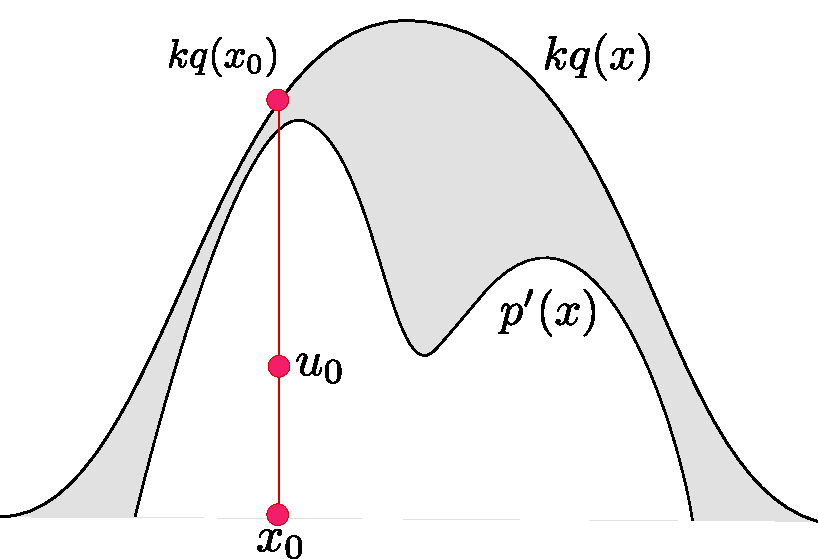
\includegraphics[scale=0.5]{./images/sampling/rejection.pdf}
		\end{center}
	\end{figure}

	The original values of $x$ are generated from the distribution $q(x)$ and these samples are then accepted with probability $p'(x)/kq(x)$ (see the figure above. The acceptance probability (\ie length) is the $p'$ divided by $kq$). Then, the probability that a sample will be accepted is given by   
	\begin{align*}
	p(accept) &= p\Bigg(u\leq \frac{p'(x)}{kq(x)}\Bigg)\\
	&= \int p\Bigg(u\leq \frac{p'(x)}{kq(x)}\bigg|x\Bigg)q(x)dx\\
	% & = \mathbb{E}[p'(x)/kq(x)] \tiny \textrm{ by Lemma 1} \\
	& = \int \frac{p'(x)}{kq(x)}q(x)dx\\
	& = \frac{1}{k}\int p'(x)dx
	\end{align*}
	Thus, the sampling will be more efficient if we choose small $k$ to increase the change of acceptance. 
%	\begin{align*}
%	p(accpet) &= \int p(accpet, x)dx\\
%	& = \int \frac{p'(x)}{kq(x)}q(x)dx\\
%	& = \frac{1}{k}\int p'(x)dx\\
%	& = \frac{1}{k}
%	\end{align*}
%	\begin{align*}
%		p(x^*) &= \frac{[p'(x^*)/kq(x^*)]q(x^*)}{\int [p'(x)/kq(x)]q(x)dx}\\
%		& = \frac{p'(x^*)}{\int p'(x^*)dx}\\
%		& = p(x^*)
%	\end{align*}

\subsection{Importance Sampling}

We want to estimate an expectation of function $f(x), x\sim p(x)$, but it would be hard to estimate the distribution $p(x)$. Again, the importance sampling is not a method for generating samples from $p(\mathbf{x})$. In this case, we can use a simple distribution $q(x)$ by
$$\mathbb{E}(f) = \int f(x)p(x)dx = \int f(x)\frac{p(x)}{q(x)}q(x)dx \approx \frac{1}{N}\sum_{n=1}^N \frac{p(x_i)}{q(x_i)}f(x_i) .$$

%Importance sampling is not a method for generating samples from $p(\mathbf{x})$. It is just a method for estimating the expectation of a function $f(\mathbf{x})$. We first generate $R$ samples $\{x^{(r)}\}$ from $q(x)$, then we could estimate the expectation by Monte Carlo method. However, if the generated samples, values of $x$ where $q(x)$ is greater than $p(x)$ will be over-represented in this estimator, and where $q(x)$ is less than $p(x)$ will be under-represented. Thus, we introduce weights 
%$$w_r = \frac{p(x^*)}{q(x^*)}$$
	
%	%$$\hat{f} = \frac{1}{L}\sum_{l=1}^{L}f(\mathbf{z}^{(l)})$$

\begin{itemize}
	\item Assume that $p(\mathbf{x})$ is known and too complicated to be sampled directly. 
	\item Samples are independently drawn from a \textbf{proposal density} $Q(\mathbf{x})$, which is designed to be close to the true density $p(\mathbf{x})$ and \textbf{simpler}
	\item Generate $R$ samples from $Q(\mathbf{x})$
\end{itemize}

\section{Gibbs Sampling}
% \label{sec:}

The phrase ``Markov chain Monte Carlo'' encompasses a broad array of techniques that have in common a few key ideas. The setup for all the techniques that we will discuss in this book is as follows:

\begin{enumerate}
	\item We want to sample from a some complicated density or probability mass function $\pi$. Often, this density is the result of a Bayesian computation so it can be interpreted as a posterior density. The presumption here is that we can evaluate $\pi$ but we cannot sample from it.
	\item We know that certain stochastic processes called Markov chains will converge to a stationary distribution (if it exists and if specific conditions are satisfied). Simulating from such a Markov chain for a long enough time will eventually give us a sample from the chain’s stationary distribution.
	\item Given the functional form of the density $\pi$, we want to construct a Markov chain that has $\pi$ as its stationary distribution.
	\item We want to sample values from the Markov chain such that the sequence of values $\{x_n\}$ generated by the chain converges in distribution to the density $\pi$.
\end{enumerate}

In order for all these ideas to make sense, we need to first go through some background on Markov chains. The rest of this chapter will be spent defining all these terms, the conditions under which they make sense, and giving examples of how they can be implemented in practice.

\subsection{Markov Chain}

A Markov chain is a stochastic process that evolves over time by transitioning into different states. The sequence of states is denoted by the collection $\{X_i\}$ and the transition between states is random, following the rule 
$$P(X_t|X_{t-1},\dots,X_0)=P(X_t|X_{t-1})$$

\begin{itemize}
	\item Each node has a probability distribution of states.
	\item Each link represents a probability state transition.  
		% \begin{align*}
		% 	P(X_1=i) = \sum_{i=1}^N P(X_i=j|X_0=i)P(X_0=i)\\
		% \end{align*}
\end{itemize}

\begin{itemize}
	\item $i \to j$: Accessible if a state $j$ is accessible from $i$. 
		\begin{itemize}
			\item $i \leftrightarrow j$: Communicate between the two states.
		\end{itemize}
	\item Reducibility: A Markov chain is \textbf{\textit{irreducible}} if $i\leftrightarrow j, \forall i,j\in S$. Simply, if all states can visit other states, then it is irreducible. 
	\item Periodic: State $i$ has a period $d$ (\ie periodically visit the state $i$) $\leftrightarrow$ aperiodic.
	\item Transience: A state is transient if, when we leave this state, there is a non-zero probability that we will never return to it. Conversely, a state is recurrent if we know that we will return to that state, in the future, with probability 1 after leaving it (if it is not transient). 
		\begin{itemize}
			\item Stationary Distribution: A probability of being in a state s at time-step t is equal to a probability of being in the state s at the next time-step. Then, it is a stationary probability distribution.
		\end{itemize}
	\item Ergodicity: A state is ergodic if the state is recurrent, aperiodic. Markov chain is ergodic if all states are ergodic. 
\end{itemize}

\subsection{Stationary Distribution}
% The return time $RT_i = \min\{n>0: X_n=i|X_0=i\}$ is the minimum time when we observe the state $X_n$ is at $i$ after the first visit ($X_0$) at $n$. 

% Limit theorem of Markov chain:
% \begin{itemize}
% 	\item If a MC is irreducible and ergodic.
% \end{itemize}

\paragraph{Limit theorem of Markov chain}

For a Markov chain with a discrete state space and transition matrix $P$, let $\pi_*$ be such that $\pi_*P=\pi_*$. Then $\pi_*$ is a stationary distribution of the Markov chain and the chain is said to be stationary if it reaches this distribution.

The basic limit theorem for Markov chains says that, under a specific set of assumptions that we will detail below, we have 
$$||\pi_*-\pi_n|| \to 0$$
as $n\to\infty$, where $||\cdot||$ is the total variation distance between the two densities. Therefore, no matter where we start the Markov chain ($\pi_0$), $\pi_n$ will eventually approach the stationary distribution. Another way to think of this is that 
$$\lim_{n\to\infty}\pi_n(i)=\pi_*(i).$$
for all states $i$ in the state space. Note that $\pi_0$ is the probability distribution of the Markov chain at time 0. Also, $\pi_n$ denote the distribution of the chain at time $n$.

\url{https://bookdown.org/rdpeng/advstatcomp/background.html}


\paragraph{Reversible MC}
Consider a stationary ergodic Markov chain with transition probability$p(i, j)$ and stationary distribution $\pi(i)$, if we reverse the process, we will get a reversed Markov chain with transition probability$q(i, j)$: 
\begin{align*}
	q(j,i) &= P(X_m=i|X_{m+1}=j)\\
		   &= \frac{P(X_m=i,X_{m+1}=j)}{P(X_{m+1}=j)}\\
		   &= \frac{P(X_m=i|X_{m+1}=j)P(X_{m+1}=j)}{P(X_{m+1}=j)}\\
		   &= \frac{\pi(i)p(i,j)}{\pi(j)}\\
	\pi(i)p(i,j) &= \pi(j)q(j,i)
\end{align*}
If $p(i,j) = q(j,i)$, it is called time-reversible Markov chain. 

% \section{Markov Chain for Sampling}


\chapter{Topic Modeling}
\section{Latent Dirichlet Allocation}
\label{sec:topic_modeling_lda}


The assumptions of LDA:
\begin{itemize}
	\item Each topic is a distribution over words.
	\item Each document is a mixture of corpus-wide topics.
	\item Each word is sampled from one of topics. 
\end{itemize}
The LDA attempts to model the document generation process stochastically. However, we have to infer the latent structure (the distributions) of documents. 

\begin{figure}[h]
	\centering
	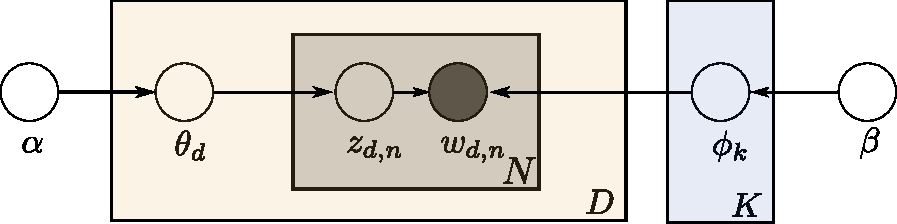
\includegraphics[scale=1.0]{./images/lda/lda.pdf}
\end{figure}
\begin{itemize}
	\item $\theta_d\sim Dir(\alpha)$: For each document, draw topic distribution. 
		\begin{itemize}
			\item $\alpha$: Dirichlet parameter
		\end{itemize}
	\item $z_{d,n}\sim Mult(\theta_d)$: per-word topic assignment. The $n$-th word of document $d$ is from which topic?
	\item $w_{d,n}\sim Mult(\phi_{z_{d,n}},n)$: observed word. The $n$-th word in a document $d$ is from a certain topic ($z_{d,n}$) distribution $\phi_{z_{d,n}}$.
	\item $\phi_k\sim Dir(\beta), i=\{1,\dots,K\}$: topics.
		\begin{itemize}
			\item $\beta$: topic hyperparameter (Dirichlet parameter).
		\end{itemize}
\end{itemize}
The document generation process can be modelled as follows:
\begin{align*}
	p(\phi_{1:K}, \theta_{1:D}, z_{1:D}, w_{1:D}) = \prod_{i=1}^K p(\phi_i|\beta)\prod_{d=1}^D p(\theta_d|\alpha)\bigg(\prod_{n=1}^N p(w_{d,n}|\phi_{1:K},z_{d,n})p(z_{d,n}|\theta_d)\bigg).
\end{align*}

\subsection{LDA Inference}
The posterior of the latent variables given the document is
\begin{align*}
	p(\phi, \theta, \mathbf{z}|\mathbf{w}) = \frac{p(\phi, \theta, \mathbf{z},\mathbf{w})}{\int_{\phi}\int_{\theta}\sum_{\mathbf{z}}p(\phi, \theta, \mathbf{z},\mathbf{w})}
\end{align*}
\begin{itemize}
	\item The denominator is intractable
\end{itemize}
We want to estimate the topic distribution $\mathbf{z}$. 

\subsection{Dirichlet Distribution}
The Dirichlet Distribution can be considered as a extension of the beta distribution. 
\begin{align}
	p(P=\{p_i\}|\alpha_i) = \frac{\Gamma(\sum_i\alpha_i)}{\prod_i\Gamma(\alpha_i)}\prod_ip_i^{\alpha_i-1}
	\label{eq:dirichlet_dist}
\end{align}
\begin{itemize}
	\item $\sum_ip_i = 1$
	\item The posterior distribution of Dirichlet distribution is also Dirichlet distribution. 
\end{itemize}


% \part{Introduction to Machine Learning}
\chapter{Latent Variable Models}
\section{Introduction}
\subsection{Motivation of Latent Variable Models}
\label{sec:intro_motivation}
If we knew a corresponding latent variable for each observation, then modelling might be easier. Imagine, how can we find $z^* = \argmax_{z} p(\mathbf{x|z})$ for the data $\mathbf{x}$ as shown in Fig. \ref{fig:clusters}(b)

\begin{figure}[h]
	\begin{center}			
		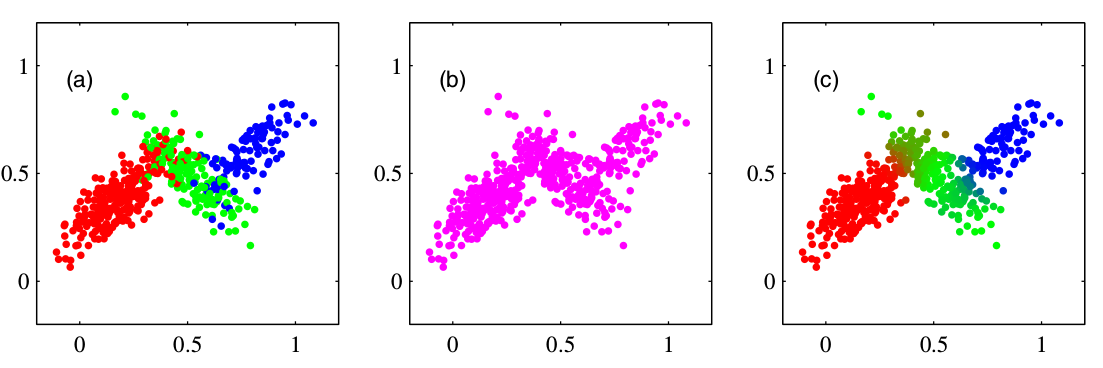
\includegraphics[scale=0.25]{./images/generative/latent.png}
	\end{center}
	\caption{(a) Complete data set $p(\mathbf{x|z})$. (b) Incomplete data set $p(\mathbf{x})$. (c) Inference result}
	\label{fig:clusters}
\end{figure}
For example, we want to model the complete data set $p(\mathbf{x|z})$ under the i.i.d. assumption 
\begin{equation*}
p(\mathbf{x}_i, \mathbf{z}_i|\boldsymbol{\theta}) = 
\begin{cases}
p(\mathcal{C}_1)p(\mathbf{x}_i|\mathcal{C}_1) \textrm{ if } z_i=0\\
p(\mathcal{C}_2)p(\mathbf{x}_i|\mathcal{C}_2) \textrm{ if } z_i=1\\
p(\mathcal{C}_3)p(\mathbf{x}_i|\mathcal{C}_3) \textrm{ if } z_i=2\\
\end{cases}
\end{equation*}
\begin{align*}
p(\mathbf{x}_1, \mathbf{x}_2,...,\mathbf{x}_N, \mathbf{z}_1, \mathbf{z}_2, ..., \mathbf{z}_N|\boldsymbol{\theta}) = \prod_{n=1}^{N}\prod_{k=1}^{K}\pi_k^{z_{nk}}\mathcal{N}(\mathbf{x}_n|\boldsymbol{\mu}_k, \boldsymbol{\Sigma}_k)^{z_{nk}}
\end{align*}
, where $\pi_k=p(\mathcal{C}_k)$ and $p(\mathbf{x}_i|\mathcal{C}_k)=\mathcal{N}(\mathbf{x}_n|\boldsymbol{\mu}_k, \boldsymbol{\Sigma}_k)$. However, in many cases, it is not observable. 

%In this case, what we can only do is find a posterior $p(\mathbf{x}|\mathbf{z},\boldsymbol{\theta})$.

\chapter{Clustering}


\section{K-Means Clustering}
Suppose we have a data set $\mathbf{X} = \{\mathbf{x}_1,...,\mathbf{x}_n\}$ consisting of $N$ observations of a random $D$-dimensional variable $\mathbf{x}\in \mathbb{R}^{D}$. Our goal is to partition the data into some number $K$ of clusters.  Intuitively, we may think of a cluster as comprising a group of data points whose inter-point distances are small compared with the distances to points outside of the cluster.

This notion can be formalized by introducing a set of $D$-dimensional vectors $\boldsymbol{\mu}_k$, which represents the centers of the clusters. Our goal is to find an assignment of data points to clusters, as well as a set of vectors $\{\boldsymbol{\mu}_k\}$. Objective function of $K$-means clustering (\textit{distortion measure}) can be defined as follows:
$$J =  \sum_{n=1}^{N}\sum_{k=1}^{K}r_{nk}||\boldsymbol{x}_n-\boldsymbol{\mu}_k||^2$$
, where $r_{nk}\in\{0,1\}$ is a binary indicator variable which represents the \textbf{membership of data} $\mathbf{x}_n$. Our goal is to find values for the $\boldsymbol{\mu}_k$ and the $r_{nk}$ so as to minimize $J$. 

We can minimize $J$ through an iterative procedure in which each iteration involves two successive steps corresponding to successive optimizations with respect to the $\boldsymbol{\mu}_k$ and the $r_{nk}$ First we choose some initial values for the $\boldsymbol{\mu}_k$. Then in the first phase we minimize $J$ with respect to the $r_{nk}$, keeping the $\boldsymbol{\mu}_k$ fixed. In the second phase we minimize $J$ with respect to the $\boldsymbol{\mu}_k$, keeping $r_{nk}$ fixed. This two-stage optimization is then repeated until convergence.

The $r_{nk}$ can be optimized in a closed-form solution as follows:
$$r_{nk}=\begin{cases}
1 & \textrm{if } k=\argmin_{j} ||\boldsymbol{x}_n-\boldsymbol{\mu}_j||^2\\
0 & \textrm{otherwise}
\end{cases}$$

Now consider the optimization of the $\boldsymbol{\mu}_k$ with the $r_{nk}$ held fixed. The objective function $J$ is a quadratic function of $\boldsymbol{\mu}_k$, and it can be minimized by setting its derivative with respect to $\boldsymbol{\mu}_k$ to zero giving
\begin{align*}
2\sum_{n=1}^{N}r_{nk}(\boldsymbol{x}_n-\boldsymbol{\mu}_k) = 0.
\end{align*}
We can arrange as
\begin{align*}
\boldsymbol{\mu}_k = \frac{\sum_n r_{nk}\boldsymbol{x}_n}{\sum_n r_{nk}}.
\end{align*}

% \begin{enumerate}
% 	\item Expectation (expectation of a log-likelihood give parameters): $$2\sum_{n=1}^{N}r_{nk}(\boldsymbol{x}_n-\boldsymbol{\mu}_k) = 0.$$
% 	\item Maximization (maximize parameters give a log-likelihood function): $$\boldsymbol{\mu}_k = \frac{\sum_n r_{nk}\boldsymbol{x}_n}{\sum_n r_{nk}}.$$ This updates the centroids. 
% \end{enumerate}

The denominator of $\boldsymbol{\mu}_k$ is equal to the number of points assigned to cluster $k$. The mean of cluster $k$ is essentially the same as the mean of data points $\mathbf{x}_n$ assigned to cluster $k$. For this reason, the procedure is known as the $K$-means clustering algorithm. 

The two phases of re-assigning data points to clusters and re-computing the cluster means are repeated in turn until there is no further change in the assignments. These two phases reduce the value of the objective function $J$, so the convergence of the algorithm is assured. However, it may converge to a local rather than global minimum of $J$. 

Some properties:
\begin{itemize}
	\item Hard clustering ($\leftrightarrow$ Soft clusstering)
	\item Centroid initialization issue.
	\item The number of clusters is uncertain. 
	\item Distance metric issue (\eg Euclidean?)
\end{itemize}



\newpage
\section{Gaussian Mixture Models}

\subsection{Multinomial Distribution}
$$P(X|\boldsymbol{\mu}) = \prod_{n} \prod_k \mu_k^{x_{nk}} = \prod_k\mu_k^{\sum_n x_{nk}}.$$
How to determine the MLE solution of $\boldsymbol{\mu}?$ \ie maximize$P(X|\boldsymbol{\mu})$ subject to $\mu_k\geq 0$ and $ \sum_k \mu_k = 1$. We can use the Lagrange method. 

\begin{align*}
	&\mathcal{L} = \sum_k\sum_nx_{nk}\ln \mu_k +\lambda(\sum_k\mu_k-1)\\ 
	&\frac{\partial \mathcal{L}}{\partial \mu_k} = \frac{\sum_nx_{nk}}{\mu_k}+\lambda. \\
	& \mu_k^{\textrm{ML}} = \frac{m_k}{N},
\end{align*}
where $m_k = \sum_n x_{nk}.$ We can consider the joint distribution of the quantities $m_1, \dots, m_K$, conditioned on the parameters $\boldsymbol{\mu}$ and on the total number $N$ observations: 
$$\textrm{Mult}(m_1, \dots, m_K|\boldsymbol{\mu}, N) = \binom{N}{m_1, \dots, m_K} = \frac{N!}{m_1!,\dots, m_K!}.$$
Note that the variables $m_k$ are subject to the constraint
$$\sum_k m_k = N.$$


\subsection{Multivariate Gaussian Distribution}
\begin{align*}
	\mathcal{N}(x|\mu,\sigma^2) = \frac{1}{\sqrt{2\pi\sigma^2}}\exp\bigg(-\frac{1}{2\sigma^2}(x-\mu)^2\bigg)
\end{align*}
For a $D$-dimensional vector $\mathbf{x}$, 
\begin{align*}
	\mathcal{N}(\mathbf{x}|\boldsymbol{\mu},\boldsymbol{\Sigma}) &= \frac{1}{(2\pi)^{D/2}|\boldsymbol{\Sigma}|^{1/2}}\exp\bigg(-\frac{1}{2}(\mathbf{x}-\boldsymbol{\mu})^T\boldsymbol{\Sigma}^{-1}(\mathbf{x}-\boldsymbol{\mu})\bigg)\\
	\ln\mathcal{N}(\mathbf{x}|\boldsymbol{\mu},\boldsymbol{\Sigma}) &= -\frac{1}{2}\ln|\boldsymbol{\Sigma}|-\frac{1}{2}(\mathbf{x}-\boldsymbol{\mu})^T\boldsymbol{\Sigma}^{-1}(\mathbf{x}-\boldsymbol{\mu})+C.
\end{align*}
Note that the functional dependence of the Gaussian on $\mathbf{x}$ is through the quadratic form: 
$$\Delta^2 = (\mathbf{x}-\boldsymbol{\mu})^T\boldsymbol{\Sigma}^{-1}(\mathbf{x}-\boldsymbol{\mu}).$$
The quantity $\Delta$ is called the \textit{Mahalanobis distance} from $\boldsymbol{\mu}$ to $\mathbf{x}$ and reduces to the Euclidean distance when $\boldsymbol{\Sigma}$ is the identity matrix.

Also,by using i.i.d. condition of a dataset, we can also express as follows:
\begin{align*}
	\ln\mathcal{N}(\mathbf{X}|\boldsymbol{\mu},\boldsymbol{\Sigma}) &= -\frac{N}{2}\ln|\boldsymbol{\Sigma}|-\frac{1}{2}\sum_n(\mathbf{x}_n-\boldsymbol{\mu})^T\boldsymbol{\Sigma}^{-1}(\mathbf{x}_n-\boldsymbol{\mu})+C
\end{align*}








\subsection{Gaussian Mixture Models}


K-means clustering is a hard-clustering, but in some cases soft-clustering provides a better model in practice. Gaussian mixture model assumes a simple \textbf{linear superposition} of Gaussian components, aimed at providing a richer class of density models than the single Gaussian. Let's consider a single sample case and it can be expressed as follows:
$$p(\mathbf{x})= \sum_{k=1}^{K}\pi_k\mathcal{N}(\mathbf{x}|\boldsymbol{\mu_k}, \boldsymbol{\Sigma}_k)$$
Let us introduce a $K$-dimensional binary random variable $\mathbf{z}$ having a 1-of-$K$ representation in which a particular element $z_k$ is equal to 1 and all other elements are 0. I will explain more about $\mathbf{z}$ later. It satisfied the following properties:
\begin{itemize}
	\item $z_k\in\{0,1\}$
	\item $\sum_kz_k=1$
\end{itemize}
The marginal distribution over $\mathbf{z}$ is specified in terms of the mixing coefficients $\pi_k$, such that 
$$p(z_k=1) = \pi_k$$
, where the mixing coefficients must satisfy
$$0\leq\pi_k\leq1$$
and 
$$\sum_{k=1}^{K}\pi_k = 1 $$
in order to be valid probabilities. We can also write pdf of $\mathbf{z}$ in a product of mixing coefficient because it is a 1-of-$K$ representaion.
$$p(\mathbf{z}) = \prod_{k=1}^{K}\pi_k^{z_k} = \pi_k \because z_k\in\{
0,1\}$$
Similarly, the conditional distribution of $\mathbf{x}$ given a particular $\mathbf{z}$ can be modeled to be a Gaussian distribution.
\begin{equation*}
p(\mathbf{x}|z_k=1) = \mathcal{N}(\mathbf{x}|\boldsymbol{\mu}_k, \boldsymbol{\Sigma}_k) 
\end{equation*}
Also can be represented in the form 
\begin{align*}
p(\mathbf{x}|\mathbf{z}) &= \prod_{k=1}^{K}\mathcal{N}(\mathbf{x}|\boldsymbol{\mu}_k, \boldsymbol{\Sigma}_k)^{z_k}\\
& = \mathcal{N}(\mathbf{x}|\boldsymbol{\mu}_k, \boldsymbol{\Sigma}_k) \because z_k\in\{
0,1\}
\end{align*}
Finally, marginal data distribution can be obtrained by summing the joint distribution over all possible states of $\mathbf{z}$ to give
\begin{align*}
	p(\mathbf{x}) &  = \sum_{\mathbf{z}} p(\mathbf{x},\mathbf{z})\\
	& = \sum_{\mathbf{z}} p(\mathbf{z})p(\mathbf{x}|\mathbf{z})= \sum_{z_1,...,z_K} p(z_1,...,z_K)p(\mathbf{x}|z_1,...,z_K)\\
	& = \sum_{k=1}^{K}\pi_k \mathcal{N}(\mathbf{x}|\boldsymbol{\mu}_k, \boldsymbol{\Sigma}_k) 
\end{align*}
Note that for every observed data point $\mathbf{x}_n$ there is a corresponding latent variable $\mathbf{z}_n$, which \textbf{indicates the membership of} $\mathbf{x}_n$. This can be represented as in Fig. \ref{fig:gmm}.

\begin{figure}[h]
	\begin{center}			
		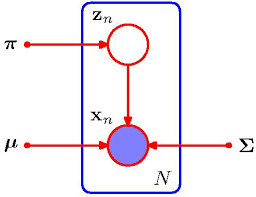
\includegraphics[scale=0.4]{./images/generative/gmm.png}
	\end{center}
	\caption{Graphical representation of GMM model. The GMM models a joint distribution $p(\mathbf{x}, \mathbf{z})$ in terms of a marginal distribution $p(\mathbf{z})$ and conditional distribution $p(\mathbf{x}|\mathbf{z})$ to model $p(\mathbf{x})$. Each $\mathbf{x}_n$ is coupled with $\mathbf{z}_n$}
	\label{fig:gmm}
\end{figure}
Now we can work with the joint distribution $p(\mathbf{x,z})$ instead of the marginal distribution $p(\mathbf{x})$, which is hard to estimate directly as explained in \Cref{sec:intro_motivation}. 

Another quantity which plays a central role is the conditional proability of $\mathbf{z}$ given $\mathbf{x}$, $p(z_k=1|\mathbf{x})$. 
\begin{itemize}
\item $p(z_k=1) = \pi_k$ can be viewed as a prior of $z_k=1$
\item $\gamma(z_k)$: assignment probability or responsibility. This represents the probability of assignment of a sample.  This quantity will be updated through the Bayes Theorem.
\item[] $\rightarrow$  A simple explanation is that \textbf{this is the classification result} of $\mathbf{x}_n$.
\end{itemize}
\begin{align*}
\gamma(z_k) \equiv p(z_k=1|\mathbf{x}) & \equiv \frac{p(z_k=1)p(\mathbf{x}|z_k=1)}{\sum_{j=1}^{K}p(z_j=1)p(\mathbf{x}|z_j=1)} \\
& = \frac{\pi_k\mathcal{N}(\mathbf{x}|\boldsymbol{\mu}_k, \boldsymbol{\Sigma}_k)}{\sum_{j=1}^{K} \pi_j\mathcal{N}(\mathbf{x}|\boldsymbol{\mu}_j, \boldsymbol{\Sigma}_j)}
\end{align*}

\subsection{Maximum Likelihood}
Suppose we have a data set of observations $\mathbf{X}=\{\mathbf{x}_1,...,\mathbf{x}_n\}^{T}\in\mathbbm{R}^{N\times D}$ and we want to model the data distribution $p(\mathbf{X})$ using GMM. If we assume an \textrm{i.i.d.} data set, it can be expressed as follows: 
\begin{align*}
p(\mathbf{X}|\boldsymbol{\pi},\boldsymbol{\mu},\boldsymbol{\Sigma}) &=\prod_{n=1}^{N}\Bigg(\sum_{k=1}^{K}\pi_k\mathcal{N}(\mathbf{x}_n|\boldsymbol{\mu}_k, \boldsymbol{\Sigma}_k)\Bigg)\\
\end{align*}
then its \textbf{loglikelihood function for GMM} is given by:
\begin{align*}
\ln p(\mathbf{X}|\boldsymbol{\pi},\boldsymbol{\mu},\boldsymbol{\Sigma}) &= \sum_{n=1}^{N}\ln \Bigg(\sum_{k=1}^{K}\pi_k\mathcal{N}(\mathbf{x}_n|\boldsymbol{\mu}_k, \boldsymbol{\Sigma}_k)\Bigg)
\end{align*}

%In a single dimension case, 
%\begin{align*}
%	\ln p(x, \pi, \mu, \sigma) & =\sum_{n=1}^{N}\ln \sum_{k=1}^{K}\pi_k \frac{1}{\sigma_k \sqrt{2\pi_k}}\exp\Big(-\frac{1}{2}\Big(\frac{x_n-\mu_k}{\sigma_k}\Big)^2\Big)\\
%	\frac{\partial }{\partial \mu_k}\ln p(x, \pi, \mu, \sigma) & =\sum_{n=1}^{N} \frac{\pi_k \frac{1}{\sigma_k \sqrt{2\pi}}\exp\Big(-\frac{1}{2}\Big(\frac{x_n-\mu_k}{\sigma_k}\Big)^2\Big) \frac{x_n-\mu_k}{\sigma_k^2}}{\sum_{k=1}^{K}\pi_k \frac{1}{\sigma_k \sqrt{2\pi}}\exp\Big(-\frac{1}{2}\Big(\frac{x_n-\mu_k}{\sigma_k}\Big)^2\Big)}\\
%	& =\sum_{n=1}^{N} \underbrace{\frac{\pi_k \mathcal{N}(x_n|\mu_k, \sigma_k) }{\sum_{k=1}^{K}\pi_k \mathcal{N}(x_n|\mu_k, \sigma_k)}}_{=\gamma(z_{nk})}\frac{x_n-\mu_k}{\sigma_k^2}\\
%	\mu_k &=\frac{1}{N_k}\sum_{n=1}^{N} \gamma(z_{nk}) x_n,
%\end{align*}
%where 
%$N_k = \sum_{n=1}^{N} \gamma(z_{nk})$. $N_k$ can be interpreted as the effective number of points assigned to cluster $k$. 

How to solve this MLE? While a gradient-based optimization is possible, we consider the iterative \textit{Expectation Maximization} algorithm.

Before, maximizing the likelihood, it is worth to emphasize two issues in GMM: (i) \textit{singularities} and (ii) \textit{identifiability}.

%\subsection{Singularity and Identifiability}
\paragraph{Singularity}
% Suppose that one of the components of the mixture model, let us say the $j$-th component, has its mean $\mathbf{\mu}_j$ exactly equal to one of the data points so that $\mathbf{\mu}_j=\mathbf{x}_n$ for some value of $n$. This data point will then contributes a term in the likelihood function of the form 
% $$\mathcal{N}(\mathbf{x}_n, \sigma_j^2\mathbf{I}) = \frac{1}{(2\pi)^{1/2}} \frac{1}{\sigma_j}$$
% If we consider the limit $\sigma_j \to 0$, then we see that this term goes to infinity and so the log likelihood function will also go to infinity. Thus the maximization of the log likelihood function will also go to infinity. Thus the maximization of the log likelihood function is not a well posed problem because such sigularities will walways be present and will occur whenever one of the Gaussian components collapses onto a specific data point. 

Before discussing how to maximize this function, it is worth emphasizing that there is a significant problem associated with the maximum likelihood framework applied to Gaussian mixture models, due to the presence of singularities. For simplicity, consider a Gaussian mixture whose components have covariance matrices given by $\Sigma_k = \sigma^2_kI$, where $I$ is the unit matrix, although the conclusions will hold for general covariance matrices. Suppose that one of the components of the mixture model, let us say the $j$-th component, has its mean $\boldsymbol{\mu}_j$ exactly equal to one of the data points so that $\boldsymbol{\mu}_j = \mathbf{x}_n$ for some value of $n$. This data point will then contribute a term in the likelihood function of the form
\begin{align*}
	\mathcal{N}(\mathbf{x}_n|\mathbf{x}_n, \sigma^2_jI) = \frac{1}{\sqrt{2\pi}\sigma_j}
\end{align*}
If we consider the limit $\sigma_j \to 0$, then we see that this term goes to infinity and so the log likelihood function will also go to infinity. Thus the maximization of the log likelihood function is not a well posed problem because such singularities will always be present and will occur whenever one of the Gaussian components `collapses' onto a specific data point. Recall that this problem did not arise in the case of a single Gaussian distribution as the variance can not be zero (recall the definition of variance). 


\paragraph{Identifiability}
A further issue in finding MLE based solutions arises from the fact that for any given maximum likelihood solution, a $K$-component mixture will have a total ok $K!$ equivalent solutions corrsponding to the $K!$ ways of assigning $K$ sets of parameters to $K$ components. In other words, for any given point in the space of parameter values there will be a further $K!-1$ additional points all of which give rise to exactly the same distribution. 

\subsection{Expectation Maximization for GMM}

The goal of Expectation Maximization (EM) is to find maximum likelihood solutions for models having latent variables 
\begin{itemize}
	\item Suppose that it is hard to optimize $p(\mathbf{X}|\boldsymbol{\theta})$ directly.
	\item However, it is easier to optimize the complete-data likelihood function $p(\mathbf{X}, \mathbf{Z}|\boldsymbol{\theta})$ 
	\item In this case, we can use \textbf{EM algorithm}. EM algorithm is a general technique for finding maximum likelihood solutions for latent variable models. 
\end{itemize}
Let us begin by writing down the conditions that must be satisfied at a maximum of the likelihood function. Setting the derivatives of $\ln p(\mathbf{X}|\boldsymbol{\pi},\boldsymbol{\mu},\boldsymbol{\Sigma})$  with respect to the means $\boldsymbol{\mu}_k$ of the Gaussian components to zero, we obtain
\begin{align*}
	0 = -\sum_{n=1}^N\frac{\pi_k\mathcal{N}(\mathbf{x}|\boldsymbol{\mu}_k, \boldsymbol{\Sigma}_k)}{\sum_{j=1}^{K} \pi_j\mathcal{N}(\mathbf{x}|\boldsymbol{\mu}_j, \boldsymbol{\Sigma}_j)}\boldsymbol{\Sigma}_k(\mathbf{x}_n-\boldsymbol{\mu}_k)
\end{align*}
Multiplying by $\boldsymbol{\Sigma}_k^{-1}$ (which we assume to be non-singular) and rearranging we obtain
\begin{align*}
	\boldsymbol{\mu}_k = \frac{1}{N_k}\sum_{n=1}^{N}\gamma(z_{nk})\mathbf{x}_n, 
\end{align*}
where we have defined
\begin{align*}
	N_k = \sum_{n=1}^{N}\gamma(z_{nk}).
\end{align*}
We can interpret $N_k$ as the effective number of points assigned to cluster $k$. We can obtain the MLE solutions for other variables similarly.
\begin{algorithm}
	Initialize the means $\boldsymbol{\mu}_k$, covariances $\boldsymbol{\Sigma}_k$ and mixing coefficients $\pi_k$ and evaluate the initial value of the log likelihood.\\
	\For{n}{
		E step: evaluate the responsibilities of $\mathbf{x}_n$ based on the current parameter values with the given parameters
		$$ \gamma(z_{nk})= p(z_k=1|\mathbf{x}_n) =  \frac{\pi_k\mathcal{N}(\mathbf{x}_n|\boldsymbol{\mu}_k, \boldsymbol{\Sigma}_k)}{\sum_{j=1}^{K} \pi_j\mathcal{N}(\mathbf{x}_n|\boldsymbol{\mu}_j, \boldsymbol{\Sigma}_j)}$$\\
		where $z_{nk}$ denote the $k$-th component of $\mathbf{z}_n$\\
		M step: maximize expectation
		\begin{itemize}
			\item $\boldsymbol{\mu}_k^{\textrm{new}} = \frac{1}{N_k}\sum_{n=1}^{N}\gamma(z_{nk})\mathbf{x}_n$
			\item $\boldsymbol{\Sigma}_k^{\textrm{new}} = \frac{1}{N_k}\sum_{n=1}^{N}\gamma(z_{nk})(\mathbf{x}_n-\boldsymbol{\mu}_k^{\textrm{new}})(\mathbf{x}_n-\boldsymbol{\mu}_k^{\textrm{new}})^T$
			\item $\pi_k^{\textrm{new}} = p(z_k=1) = \frac{N_k}{N}$
		\end{itemize}
	Evaluate the log likelihood to check for convergence of parameters
	$$\textrm{ln}p(\mathbf{X}|\boldsymbol{\pi},\boldsymbol{\mu},\boldsymbol{\Sigma}) = \sum_{n=1}^{N}\textrm{ln}\Bigg(\sum_{k=1}^{K}\pi_k\mathcal{N}(\mathbf{x}_n|\boldsymbol{\mu}_k, \boldsymbol{\Sigma}_k)\Bigg)$$
	}
	\caption{EM algorithm for GMM}
\end{algorithm}
	\begin{figure}[h]
	\begin{center}
		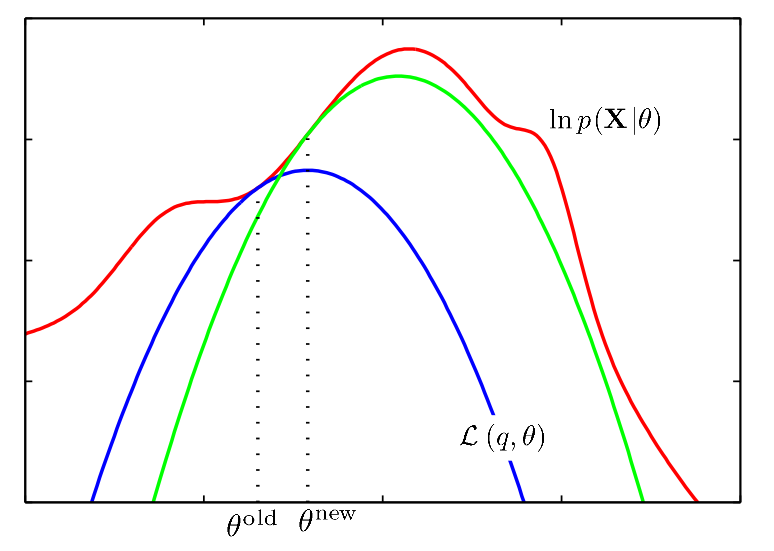
\includegraphics[scale=0.3]{./images/generative/em_update.png}
	\end{center}
	\caption{M-step of EM algorithm}
	\label{fig:em2}
\end{figure}

\section{Alternative View of EM}
The goal of the EM algorithm is to find maximum likelihood (loglikelihood) solutions for models having latent variables.
$$\ln p(X|\theta) = ln\sum_Z p(X,Z|\theta).$$
We are not given the complete data set ${X, Z}$, but only the incomplete data $X$. Our state of knowledge of the values of the latent variables
in $Z$ is given only by the posterior distribution $p(Z|X, \theta)$. Because we cannot use the complete-data log likelihood, we consider instead its expected value under the posterior distribution of the latent variable, which corresponds (as we shall see) to the E step of the EM algorithm.

In the subsequent M step, we maximize this expectation. If the current estimate for the parameters is denoted $\theta_{old}$, then a pair of successive E and M steps gives rise to a revised estimate $\theta^{new}$.

The algorithm is initialized by choosing some starting value for the parameters $\theta_0$. The use of the expectation may seem somewhat arbitrary.

In the E step, we use the current parameter values $\theta^{old}$ to find the posterior distribution of the latent variables given by $p(Z|X, \theta^{old})$. We then use this posterior distribution to find the expectation of the complete-data log likelihood evaluated for some general parameter value $\theta$. This expectation, denoted $Q(\theta, \theta^{old})$, is given by 
$$Q(\theta, \theta^{old}) = \sum_Z p(Z|X, \theta^{old})\ln p(X,Z|\theta).$$
In the M step, we determine the revised parameter estimate $\theta^{new}$ by maximizing this function
$$\theta^{new}=\argmax Q(\theta, \theta^{old}).$$


\begin{algorithm}
The goal is to maximize the likelihood function $p(X|\theta)$ with respect to $\theta$ given a joint distribution $p(X, Z|\theta)$.\\
1. Init $\theta^{old}$\\
2. E-Step: evaluate $p(Z|X, \theta^{old})$ \\
3. M-Step: evaluate $\theta^{new}$ given by 
$$\theta^{new} = \argmax Q(\theta, \theta^{old}),$$
where
$$Q(\theta, \theta^{old}) = \sum_Z p(Z|X, \theta^{old})\ln p(X,Z|\theta).$$
4. Check for convergence of either the log likelihood or the parameter values. If the convergence criterion is not satisfied, then let
$$\theta^{old}\leftarrow \theta^{new}.$$
Return to the step 2. 
\caption{General EM algorithm}
\end{algorithm}



\section{Latent Variable Modeling}

For each object $x_i$, we establish additional latent variable $z_i$ which denotes the index of gaussian from which $i$-th object was generated. Then our model is
$$p(X,Z|\theta) = \prod_{i=1}^{n}p(x_i,z_i|\theta) = \prod_{i=1}^{n}p(x_i|z_i,\theta)p(z_i|\theta) = \prod_{i=1}^{n}\mathcal{N}(x_i|\mu_{z_i},\sigma_{z_i}^2)\pi_{z_i},$$
where $\pi_{j} = p(z_i=j)$ are prior probability of $j$-th gaussian and $\theta = \{\mu_j, \sigma_j, \pi_j\}_{j=1}^K$. If we know both $X$ and $Z$ then we can obtain explicit ML-solution:
$$\theta_{ML} = \argmax_{\theta}p(X,Z|\theta) = \argmax_{\theta}\log p(X,Z|\theta).$$
However, in practice, we don't know $Z$, but only know $X$. Thus, we need to maximize w.r.t. $\theta$ the log of incomplete likelihood
\begin{align}
	\log p(X|\theta) & = \ln \int  p(X, Z|\theta)dZ\\
					 & = \ln\int q(Z|X) \frac{p(X, Z|\theta)}{q(Z|X)}dZ\\
					 & \geq \underbrace{\int q(Z|X) \ln\frac{p(X, Z|\theta)}{q(Z|X)}dZ}_{\textrm{ELBO, } \mathcal{L}(q,\theta)} \quad\textrm{by Jensen's Inequality.}\\
					 &= \int q(Z|X) \ln p(X, Z|\theta) - q(Z|X)\ln q(Z|X)dZ\\
					 &= \int q(Z|X)[\ln p(X|Z,\theta) + \ln p(Z|\theta)]  - q(Z|X)\ln q(Z|X)dZ\\
					 &= \int q(Z|X)\ln p(X|Z,\theta)  - q(Z|X)\ln\frac{q(Z|X)}{p(Z|\theta)}dZ\\
					 &= \mathbb{E}_{q(Z|X)} \ln p(X|Z,\theta)  - KL(q(Z|X)||p(Z|\theta)) 
	% & = \int q(Z)\log \frac{p(X,Z|\theta)}{p(Z|X,\theta)}dZ\\
	% & = \int q(Z)\log \frac{q(Z)p(X,Z|\theta)}{q(Z)p(Z|X,\theta)}dZ\\
	% & = \int q(Z)\log \frac{p(X,Z|\theta)}{q(Z)}dZ+ \int q(Z)\log \frac{q(Z)}{p(Z|X,\theta)}dZ\\
	% & = \underbrace{\int q(Z)\log \frac{p(X,Z|\theta)}{q(Z)}dZ}_{\textrm{ELBO, } \mathcal{L}(q,\theta)}+ \textrm{KL}(q(Z)||\log p(Z|X,\theta))
	\label{eq:elbo}
\end{align}
% Note that $\textrm{KL}( \cdot|| \cdot)\geq 0$, thus $\mathcal{L}(q,\theta) \leq \log p(X|\theta)$. In other words, $\mathcal{L}(q,\theta)$ is a \textbf{lower bound} on $\log p(X|\theta)$.

% Let's see ELBO in a different perspective
% \begin{align*}
% 	\mathcal{L}(q,\theta) &=  \int q(Z)\log \frac{p(X,Z|\theta)}{q(Z)}dZ\\
% 	&= \int q(Z)\Big[\log p(X,Z|\theta)- \log q(Z)\Big]dZ\\
% 	&= \int q(Z)\Big[\log p(Z|X,\theta)+\log p(X|\theta)-\log q(Z)\Big]dZ\\
% 	&= \int q(Z)\log p(X|\theta)dZ+\int q(Z) \log\frac{ p(Z|X,\theta)}{ q(Z)}dZ\\
% 	&= \log p(X|\theta)-\textrm{KL}(q(Z)||p(Z|X,\theta))
% \end{align*}
To maximize the above equation, we need to minimize KL divergence. 

% Also note that $p$ does not depend of $q$, \textbf{so maximizing ELBO is equal to minimizing the KL divergence}. 

% By using ELBO, we are able to maximize the incomplete likelihood. If you see the KL term, it is trying to minimize the divergence between $q(Z)$ and $p(Z)$ through maximizing ELBO.


\subsection{Evidence Lower Bound (ELBO)}
For any choice of inference model $q_{\phi}(z|x)$, we can represent the marginal probability of data (or model evidence) distribution, since the $z$ is not related to $x$, so the integration does not affect $x$. Thus, we can also derive ELBO as follows:
\begin{align*}
	\log p_{\theta}(x) &= \mathbb{E}_{q_{\phi}(z|x)}[\log p_{\theta}(x)]\\
	& = \mathbb{E}_{q_{\phi}(z|x)}\Bigg[\log \frac{p_{\theta}(x,z)}{p_{\theta}(z|x)}\Bigg]\\
	& = \mathbb{E}_{q_{\phi}(z|x)}\Bigg[\log \frac{p_{\theta}(x,z)q_{\phi}(z|x)}{q_{\phi}(z|x) p_{\theta}(z|x)}\Bigg]\\
	& = \underbrace{\mathbb{E}_{q_{\phi}(z|x)}\Bigg[\log \frac{p_{\theta}(x,z)}{q_{\phi}(z|x) }\Bigg]}_{=\mathcal{L}(\phi,\theta)(x)}+\underbrace{ \mathbb{E}_{q_{\phi}(z|x)}\Bigg[\log \frac{q_{\phi}(z|x)}{p_{\theta}(z|x)}\Bigg]}_{=D_{KL}(q_{\phi}(z|x)||p_{\theta}(z|x))}
\end{align*}

To get more intuition about ELBO, we can express ELBO as follows:
\begin{align*}
	\mathcal{L}(\phi,\theta) & = \mathbb{E}_{q_{\phi}(z|x)}\Bigg[\log \frac{p_{\theta}(x,z)}{q_{\phi}(z|x) }\Bigg]\\
	& = \mathbb{E}_{q_{\phi}(z|x)}\Bigg[\log p_{\theta}(x,z)-\log q_{\phi}(z|x)\Bigg]\\
	& = \mathbb{E}_{q_{\phi}(z|x)}\Bigg[\log p_{\theta}(x)+\log p_{\theta}(z|x)-\log q_{\phi}(z|x)\Bigg]\\
	& = \log p_{\theta}(x) - D_{\textrm{KL}}(q_{\phi}(z|x)||p_{\theta}(z|x))\\
	& \leq \log p_{\theta}(x)
\end{align*}

ELBO can be also written as follows:
\begin{align*}
\mathcal{L}(\phi,\theta) & = \mathbb{E}_{q_{\phi}(z|x)}\Bigg[\log \frac{p_{\theta}(x,z)}{q_{\phi}(z|x) }\Bigg]\\
& = \mathbb{E}_{q_{\phi}(z|x)}\Bigg[\log p_{\theta}(x,z)-\log q_{\phi}(z|x)\Bigg]\\
& = \mathbb{E}_{q_{\phi}(z|x)}\Bigg[\log p_{\theta}(z)+\log p_{\theta}(x|z)-\log q_{\phi}(z|x)\Bigg]\\
& = \mathbb{E}_{q_{\phi}(z|x)}[\log p_{\theta}(x|z)] - D_{\textrm{KL}}(q_{\phi}(z|x)||p_{\theta}(z))\\
\end{align*}

We can get a conclusion that maximizing ELBO is equivalent to minimizing the KL divergence through the above equation. Fianlly, the log-likelihood can be rewritten as follows:
\begin{align*}
	\log p_{\theta}(x) = \mathcal{L}(\phi,\theta) + D_{\textrm{KL}}(q_{\phi}(z|x)||p_{\theta}(z|x))
\end{align*}


%\section{Variational Lower Bound}
%Function $g(\xi, x)$ is called variational lower bound for function $f(x)$ iff
%\begin{itemize}
%	\item For all $\xi$ for all $x$ if follows $f(x)\geq g(\xi, x)$
%	\item For any $x_0$ there exists $\xi(x_0)$ such that $f(x_0)=g(\xi(x_0), x_0)$
%\end{itemize} 

\subsection{Expectation Maximization}
We want to maximize ELBO, $\mathcal{L}(q,\theta)$ to minimize KL divergence between $q(Z)$ and $\log p(Z|X,\theta)$.
$$\max_{q,\theta}\mathcal{L}(q,\theta) = \max_{q,\theta}\int q(Z)\log \frac{p(X,Z|\theta)}{q(Z)}dZ.$$
We start from initial point $\theta_0$ and iteratively repeat \Ni E-step and \Nii M-step, iteratively:
\begin{itemize}
	\item E-Step: $\theta_0$ is fixed. 
		$$q(Z) = \argmax_{q}\mathcal{L}(q,\theta) = \argmin_{q}\textrm{KL}(q(Z)|p(Z|X,\theta)) = p(Z|X,\theta_0).$$ 
		\begin{itemize}
			\item This is because, maximizing ELBO is equal to minimizing KL divergence and the minimum $q$ can be achieved when $q$ is equal to $p(Z|X,\theta_0)$.
			\item Now, we just have to evaluate $p(Z|X,\theta_0)$.
		\end{itemize}
	\item M-Step: $q$ is fixed.
		$$\theta_* = \argmax_{\theta}\mathcal{L}(q,\theta) = \argmax_{\theta}\mathbb{E}_{q(Z)}[\log p(X,Z|\theta)]$$
		\begin{itemize}
			\item Can be accomplished by taking derivatives
			\item Set $\theta_0=\theta_*$ and go to the E-Step until convergence
		\end{itemize}
	
\end{itemize}

\subsection{Categorical Latent Variables}
$z_i \in \{1,...,K\}$
$$p(x_i|\theta) = \sum_{k=1}^{K}p(x_i|k,\theta)p(z_i=k|\theta)$$
is simply a finite mixture of distributions. 

E-Step:
$$q(z_i=k) = p(z_i=k|x_i,\theta) = \frac{p(x_k|z_i=k,\theta)p(z_i=k|\theta)}{\sum_{l=1}^{K}p(x_i|z_i=l,\theta)p(z_i=l|\theta)}$$
M-Step:
$$\argmax_{\theta}\mathbb{E}_{q(Z)}[\log p(X,Z|\theta)] = \sum_{i=1}^{n}\mathbb{E}_{q(z_i)}[\log p(x_i,z_i|\theta)] = \sum_{i=1}^{n}\sum_{k=1}^{K}q(z_i=k)\log p(x_i,k|\theta)$$

For GMM, we model $p(x|z)$ as Gaussian.

%\subsection{Continous Latent Variables}
%Continuous latent variables can be regarded as a mixture model of continous distributions. 
%$$p(x_i|\theta) = \int p(z_i|x_i,\theta) dz_i = \int p(x_i|z_i,\theta)p(z_i|\theta) dz_i$$
%E-step can be done in a closed from only in case of conjugate distributions, otherwise the true posterior is intractadble.
%$$q(z_i) = p(z_i|x_i,\theta) = \frac{p(x_k|z_i,\theta)p(z_i|\theta)}{\int p(x_i|z_i,\theta)p(z_i|\theta)dz_i}$$
%
%Typically, continuous latent variables are used for dimension reduction techniques also known as \textbf{representation learning.}

% \part{Deep Generative Models}
\chapter{Explicit Generative Models}
\section{Variational Autoencoder}

Our goal is to find the data distribution $p(X)$. \Cref{fig:dgm} represents a general structure of deep generative model. As you can see, we first sample $z\sim p(z)$ and feed it into a deep neural network $f(z)$ and output $x$.

\begin{figure}[h]
	\begin{center}
		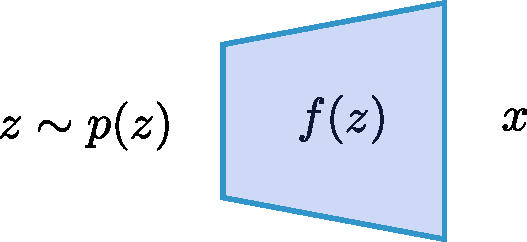
\includegraphics[scale=0.5]{./images/generative/dgm.pdf}
	\end{center}
	\caption{General structure of deep generative models. This model does not infer $z$ from $x$.}
	\label{fig:dgm}
\end{figure}

VAE performs an inference by introducing a probabilistic encoder, called inference network. VAEs are generative model with a latent variable distributed according to some distribution $p(z_i)$. The observed variable is distributed according to a conditional distribution 
$$p_\theta(x_i|z_i)$$
This conditioning means the latent variable values are the one most likely given the observations. We also create a distribution $q_\phi(z_i|x_i)$. We would like to be able to encode our data into the latent variable space. Let's model the distribution.

\begin{itemize}
	\item $p_\theta(x_i|z_i)\sim \mathcal{N}(x_{i}|\mu(z_i), \sigma^2(z_i))$: A probabilistic decoder (or generative network, $\theta$)
	\item $q_\phi(z_i|x_i)$: A probabilistic encoder (or inference network $\phi$). We can choose a family of distributions for our conditional distribution $q$ (\eg standard Gaussian distribution). 
		$$q_\phi(z_i|x_i) = \mathcal{N}(z_i|\mu(x_i, W_1), \sigma^2(x_i, W_2)I),$$
	where $W_1$ and $W_2$ are network weights and collectively denoted as $\phi$. We create a neural network to model the distribution $q$ from our data in a non-linear manner. The outputs of the network are $\mu$ and $\sigma$. 
\end{itemize}

\begin{figure}[h]
	\begin{center}
		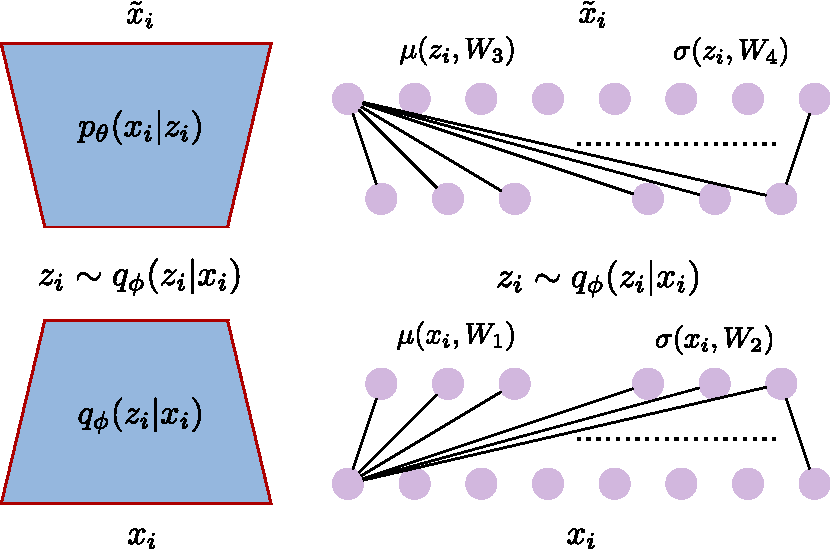
\includegraphics[scale=0.5]{./images/generative/encoder.pdf}
	\end{center}
	\caption{Overview of variational autoencoder.}
	\label{fig:vae}
\end{figure}



\begin{align*}
	p(X,Z|\theta) &=  \prod_{i=1}^{n}\underbrace{p(x_i|z_i,\theta)}_{\textrm{Likelihood, Generator}}\underbrace{p(z_i|\theta)}_{\textrm{Prior on latent variable}}\\
	&= \prod_{i=1}^{n} \mathcal{N}(x_{i}|\underbrace{\mu(z_i), \sigma^2(z_i)}_{\textrm{Non-linear}}) \mathcal{N}(z_i|0, I)
\end{align*}

Subsequently, marginal distributions can be expressed as follows under i.i.d. assumption:
\begin{align*}
	p(X|\theta) &= \prod_{i=1}^{n} p(x_i|\theta) \\
	&= \prod_{i=1}^{n} \int p(x_i, z_j|\theta) dz_j \\
	& = \prod_{i=1}^{n} \int p(x_i|z_i, \theta)p(z_i|\theta)dz_i \\
	& = \prod_{i=1}^{n} \int \mathcal{N}(x_{i}|\mu(z_i), \sigma^2(z_i)) \underbrace{\mathcal{N}(z_i|0, I)}_{\textrm{Mixture weight}} dz_i
\end{align*}

\begin{itemize}
	\item As you can see, the marginal distribution $p(X|\theta)$ becomes a mixture of Gaussian (infinite mixture of Gaussian). 
	\item Even though $p(x|z)$ and $p(z)$ are normal, $p(x)$ is not normal, because it is a mixture distribution.
	\item The non-linearity of Gaussian parameters (modeled by a neural network), conjugacy between the prior and the likelihood does not hold anymore.
%	\item Diagonal covariance matrix does not mean the independence between elements of $x$.
	\item Again, $\mu$ and $\sigma$ is non-linear function of $z$ modeled by some non-linear neural network. The neural network works as a powerful non-linear parameter approximator (based on universal approximation theorem). 
	\item Simple prior is used. Let's consider the data $x$ is an image of $100\times 100$ pixels. Then the covariance matrix has to be $10000\times 10000$. Thus, it is common to set a simple prior such as the standard Gaussian (covariance matrix is diagonal matrix). However, even if we set a simple distribution, with the infinite mixture of Gaussian, we can model any distribution.
	\item VAE uses a global parametric model to predict the local
		variational parameters for each data point (\textbf{amortized inference}). 
%	\item Under the simple standard Gaussian prior assumption, the generator, $p(x_i|z_i,\theta)$, returns factorized Gaussian whose mean and variance are non-linear functions of latent variable modelled by deep neural network parameterized by $\theta$.
%	$$p(x_i|z_i,\theta) = \mathcal{N}(x_{i}|\mu(z_i), \sigma^2(z_i))$$
%	\item VAEs uses a simple prior over latent variables and complicated and powerful generator (neural network).
	\item It allows to convert complicated large-dimensional data distributions into simple lower-dimensional latent variable representations.  
%	\item $Std = e^{\frac{1}{2}\log (Var)}$, thus output is the log var
\end{itemize}

\subsection{VAE Optimization}
We can train VAE using variational inference with the following objective function, ELBO:
$$\mathcal{L}(\phi,\theta) = \mathbbm{E}_{q_{\phi}(z|x)}[\log p_{\theta}(x|z)] - D_{\textrm{KL}}(q_{\phi}(z|x)||p_{\theta}(z))$$
Let's closely look at this objective function:
\begin{itemize}
	\item In $q_{\phi}(z|x)$, $x$ is a given data, so it is not stochatic. How to sample $z$?
	\item $q$ has to be deterministic and differentiable. 
	\item[] $\to$ \textbf{Reparameterization trick}!
		$$\tilde{z}\sim q_\phi(z|x) \to \tilde{z}\sim g_{\phi}(\epsilon, x)$$, where $\epsilon\sim p(\epsilon).$

	\item Estimated by using Monte-Carlo estimation 
		$$\mathbbm{E}_{q_{\phi}(z|x)}[\log p_{\theta}(x|z)]\approx \frac{1}{N}\sum_j \log p_{\theta}(x_i|z_j).$$
\end{itemize}

\subsection{Conditional VAE}
If we have label information about data, then it would provide a better optimization of VAE model. Recall that the following objective function is the objective of the original VAE:
$$\mathcal{L}(\phi,\theta) = \mathbbm{E}_{q_{\phi}(z|x)}[\log p_{\theta}(x|z)] - D_{\textrm{KL}}(q_{\phi}(z|x)||p_{\theta}(z))$$
In conditional VAE, 
$$\mathcal{L}(\phi,\theta) = \mathbbm{E}_{q_{\phi}(z|x, y)}[\log p_{\theta}(x|y, z)] - D_{\textrm{KL}}(q_{\phi}(z|x, y)\ ||\ p_{\theta}(z|y))$$

\begin{align}
	\log p(X|Y) & = \ln\int q(Z|X, Y) \frac{p(X, Z|Y)}{q(Z|X, Y)}dZ\\
					 & \geq \underbrace{\int q(Z|X, Y) \ln\frac{p(X, Z|Y)}{q(Z|X, Y)}dZ}_{\textrm{ELBO, } \mathcal{L}(q,\theta)} \quad\textrm{by Jensen's Inequality.}\\
					 &\dots\\
					 &\dots\\
					 &= \mathbb{E}_{q(Z|X,Y)} [\ln p(X|Z,Y)]  - KL(q(Z|X,Y)||p(Z|Y)) 
	% & = \int q(Z)\log \frac{p(X,Z|\theta)}{p(Z|X,\theta)}dZ\\
	% & = \int q(Z)\log \frac{q(Z)p(X,Z|\theta)}{q(Z)p(Z|X,\theta)}dZ\\
	% & = \int q(Z)\log \frac{p(X,Z|\theta)}{q(Z)}dZ+ \int q(Z)\log \frac{q(Z)}{p(Z|X,\theta)}dZ\\
	% & = \underbrace{\int q(Z)\log \frac{p(X,Z|\theta)}{q(Z)}dZ}_{\textrm{ELBO, } \mathcal{L}(q,\theta)}+ \textrm{KL}(q(Z)||\log p(Z|X,\theta))
\end{align}
Note that not we have a prior $p_{\theta}(z|y)$. However, we have no idea about latent variable $z$, so we simply assume that we cannot impact the $z$ by $y$. Thus, we typically set it as a standard normal distribution. Also, we can simply concatenate the input $X$ with $Y$. 

\subsection{Variational Deep Embedding (VaDE)}
The generative process of VADE $p(x, z, c) = p(x|z)p(z|c)p(c)$:
\begin{itemize}
	\item Choose a cluster $c\sim Cat(\pi)$
	\item Choose a latent vector $z\sim \mathcal{N}(\mu_c, \sigma_c^2I)$
	\item Choose a sample $x$:
		\begin{align*}
			x\sim
			\begin{cases}
				Ber(\mu_x)\quad &\textrm{If }$x$ \textrm{ is binary} \\
				\mathcal{N}(\mu_x, \sigma_x^2I) \quad &\textrm{else}
			\end{cases}
		\end{align*}
\end{itemize}
ELBO of VaDE:
\begin{align}
	\log p(X) & = \ln\int \sum_c p(X,Z,C) dz \\
					 & \geq \underbrace{\int q(Z,C|X) \ln\frac{p(X, Z, C)}{q(Z,C|X)}dZ}_{\textrm{ELBO}} 
\end{align}
The ELBO can be decomposed as follows:
\begin{align*}
\mathcal{L}_{ELBO} &= \mathbb{E}_q(z,c|x)\bigg[\ln\frac{p(x,z,c)}{q(z,c|x)}\bigg]\\
				   &= \mathbb{E}_q(z,c|x)[\ln p(x,z,c) - \ln q(z,c|x)]\\
				   &= \mathbb{E}_q(z,c|x)[\ln p(x|z) + \ln p(z|c)+ \ln p(c)-\ln q(z|x)-\ln q(c|x)]
\end{align*}
By using two factorizations:
\begin{itemize}
	\item $p(x, z, c) = p(x|z)p(z|c)p(c)$
	\item $q(z,c|x) \approx q(z|x)q(c|x)$ (Mean-field assumption)
		\begin{itemize}
			\item $q(z|x)\sim \mathcal{N}$: encoder, estimate mean and variance.
			\item $q(c|x)$: assignment probability of Gaussian mixture model
		\end{itemize}
\end{itemize}

\subsection{Importance Weighted VAE}


% \begin{itemize}
% 	\item 
% 		$$\mathbbm{E}_{q_{\phi}(z|x)}[\log p_{\theta}(x|z)]\approx \frac{1}{N}\sum_j \log p_{\theta}(x_i|z_j).$$
% 	\item The second term can be solve analytically for some distributions like Gaussian.
% 	\item For training, we need to use a reparameterization trick. 
% \end{itemize}




%\footnotetext[1]{Uncorrelated relationship does not imply the independence (independence makes covariance to be diagonal). If two variables are uncorrelated, $Cov(x_i,x_j)=0 $, there is no linear relationship between them.}
%\footnotetext[2]{In practice, simple prior could be a problem.}

\chapter{Implicit Generative Models}
\section{Generative Adversarial Networks}
\label{sec:gan}
\begin{itemize}
	\item Generator's distribution: $p_{g}$
	\item Prior on input noise: $p_{z}(z)$
	\item Mapping to data space: $z\rightarrow x$ through $G(z;\theta_{g})$
	\item[] a differentiable multilayer perceptron with parameter $\theta_{g}$
	\item $D(x;\theta_{d})$: a differentiable multilayer perceptron with parameter $\theta_{d}$. It outputs a single scalar 
	\item $D(x)$: probability that $x$ (real) came from the data rather than $p_g$ (fake)
\end{itemize}

\begin{figure}[h]
	\begin{center}
		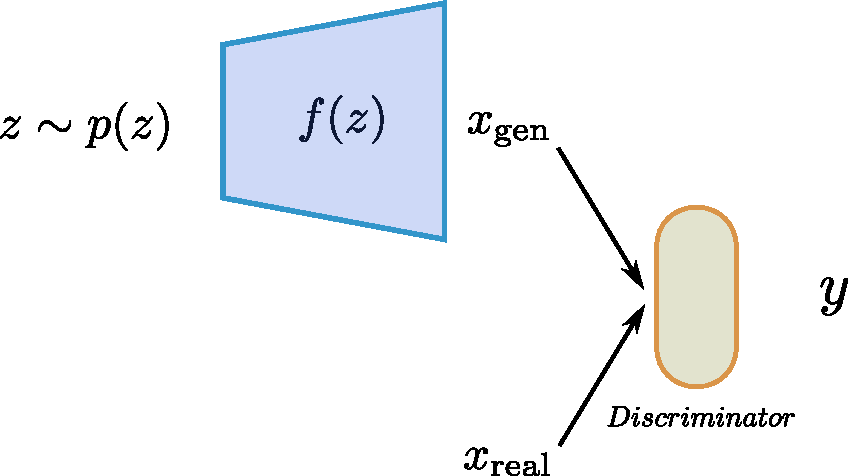
\includegraphics[scale=0.5]{./images/generative/gan/gan_model.pdf}
	\end{center}
	\caption{GAN structure}
	\label{fig:gan}
\end{figure}

\subsection{Discriminator}
The discriminator's goal is to maximize the following equation given $G$
\begin{equation*}
\mathbbm{E}_{x \sim p_{data}(x)}\log(D(x))+\mathbbm{E}_{z \sim p_{z}(z)}\log(1-D(G(z)))
\end{equation*}
The optimal discriminator given $G$ can be denoted as $D^*_{G}$. To get the optimal discriminator, define a value function
\begin{equation*}
V(G,D):= \mathbbm{E}_{x \sim p_{data}(x)}\log(D(x))+\mathbbm{E}_{z \sim p_z(z)}\log(1-D(G(z))).
\end{equation*}
Then, $D_G^* = \text{argmax}_D V(G,D)$

However, the generator $G$ wants to minimize the value function given $D=D^*_G$. 
\begin{equation*}
G^* = \text{argmin}_G V(G,D_G^*).
\end{equation*}

\begin{equation*}
\min_{G}\max_{D}V(D,G) =  \mathbbm{E}_{x\sim p_{data}(x)}[\textrm{log}D(x)]+\mathbbm{E}_{z\sim p_{z}(z)}[\textrm{log}(1-D(G(z)))]
\end{equation*}
\begin{itemize}
	\item $\min_{G} \rightarrow$ try to generate fake data that is similar to real data
	\item $\max_{D} \rightarrow$ try to assign correct label \footnotemark
\end{itemize}

At this point, we must show that this optimization problem has a unique solution $G^*$ and that this solution satisfies $p_G=p_{data}$.

\footnotetext{The above equation is trained separately at the same time, don't get confused}

One big idea from the GAN paper–, which is different from other approaches is that $G$ \textbf{need not be invertible}. Many pieces of notes online miss this fact when they try to replicate the proof and incorrectly use the change of variables formula from calculus (which would depend on $G$ being invertible). Rather, the whole proof relies on this equality:
\begin{equation*}
	\mathbbm{E}_{z \sim p_{z}(z)}\log(1-D(G(z))) = \mathbbm{E}_{x \sim p_{G}(x)}\log(1-D(x)) .
\end{equation*}

With the above equality, 
\begin{align*}
	&\mathbbm{E}_{x \sim p_{data}(x)}\log(D(x))+\mathbbm{E}_{z \sim p_z(z)}\log(1-D(G(z)))\\
	&=\int_{x} p_{data}(x)\log D(x) \, \mathrm{d}x + \int_{z} p(z)\log ( 1- D(G(z))) \, \mathrm{d}z\\ 
	&= \int_{x} p_{data}(x)\log D(x) + p_G(x) \log ( 1- D(x)) \, \mathrm{d}x
\end{align*}

Additionally, we will use the following property:
\begin{align*}
	f(y)= a \log y + b \log(1-y).
\end{align*}
To find a critical point,
$$f^\prime(y) = 0 \Rightarrow \frac{a}{y} - \frac{b}{1-y} = 0 \Rightarrow y = \frac{a}{a+b}$$
If $a+b\neq0$, do the second derivative test:
$$f^{\prime\prime}\big ( \frac{a}{a+b} \big) = - \frac{a}{(\frac{a}{a+b})^2} - \frac{b}{(1-\frac{a}{a+b})^2} < 0
$$
If $a,b\in (0,1)$, $\frac{a}{a+b}$ is a maximum.

By rewriting the equation,
\begin{align*}
V(G,D) &= \int_{x} p_{data}(x)\log D(x) + p_G(x) \log ( 1- D(x)) \, \mathrm{d}x \\
& \leq \int_x \max_y {p_{data}(x)\log y + p_G(x) \log ( 1- y)}\, \mathrm{d}x 
\end{align*}
Thus, if $D(x) = \frac{p_{data}}{p_{data}+p_G}$, then we can achieve the maximum $V(G,D)$. 

\subsection{Generator}
If we achieve the optimal $G$ (i.e., $p_G = p_{data}$), then $D$ would be completely confused and $D^*_G(x) = \frac{p_{data}}{p_{data}+p_G}=\frac{1}{2}$ (it means that $D$ cannot make a clear decision.).

The global minimum of the virtual training criterion $C(G)=\max_DV(G,D)$ is acheived if and only if $p_{G}=p_{data}$. Let's plug $D^*_G(x)$ into the criterion then, 
\begin{equation*}
	C(G) = \int_{x} p_{data}(x)\log \big (\frac{p_{data}(x)}{p_{G}(x)+p_{data}(x)} \big )  + p_G(x) \log\big ( \frac{p_{G}(x)}{p_{G}(x)+p_{data}(x)}\big ) \, \mathrm{d}x. 
\end{equation*}
To get the minimum $C(G)$, we can use the Jansen-Shannon divergence:

\begin{align*}
	D_{JS}(p_{data}||p_{G}) & = \frac{1}{2}\Bigg[D_{KL}\Big(p_{data}\Big|\Big|\frac{p_{data}+p_{G}}{2}\Big)+D_{KL}\Big(p_{G}\Big|\Big|\frac{p_{data}+p_{G}}{2}\Big)\Bigg]\\
	& = \frac{1}{2}\Bigg[\Bigg(\int_x p_{data}(x)\textrm{log}\Bigg(\frac{2p_{data}(x)}{p_{data}(x)+p_{G}(x)}\Bigg)dx\Bigg)+\Bigg(\int_x p_{G}(x)\textrm{log}\Bigg(\frac{2p_{G}(x)}{p_{data}(x)+p_{G}(x)}\Bigg)dx\Bigg)\Bigg]\\
	& = \frac{1}{2}\Bigg[\Bigg(\int_x p_{data}(x)\textrm{log}2+p_{data}(x)\textrm{log}\Bigg(\frac{p_{data}(x)}{p_{data}(x)+p_{G}(x)}\Bigg)dx\Bigg)+\\
	&\hspace{1cm}\Bigg(\int_x p_{G}(x)\textrm{log}2+p_{G}(x)\textrm{log}\Bigg(\frac{p_{G}(x)}{p_{data}(x)+p_{G}(x)}\Bigg)dx\Bigg)\Bigg]\\
	& = \frac{1}{2}\Bigg[\Bigg(\textrm{log}2+\int_x p_{data}(x)\textrm{log}\Bigg(\frac{2p_{data}(x)}{p_{data}(x)+p_{G}(x)}\Bigg)dx\Bigg)+\\
	& \hspace{1cm}\Bigg(\textrm{log}2+\int_x p_{G}(x)\textrm{log}\Bigg(\frac{2p_{G}(x)}{p_{data}(x)+p_{G}(x)}\Bigg)dx\Bigg)\Bigg]\\
	& = \frac{1}{2}(\textrm{log}4+C(G))
\end{align*}

Thus,
$$C(G) = -\textrm{log}4 + 2D_{JS}(p_{data}||p_{G})$$

Since the Jensen-Shannon divergence between two distributions is always non-negative and zero only when they are equal, we have shown that $C^* = -\textrm{log}(4)$ is the global minimum of $C(G)$ and that the only solution is $p_G=p_{data}$, i.e., the generative model perfectly replicating the data generating process.

\begin{figure}[h]
	\centering
	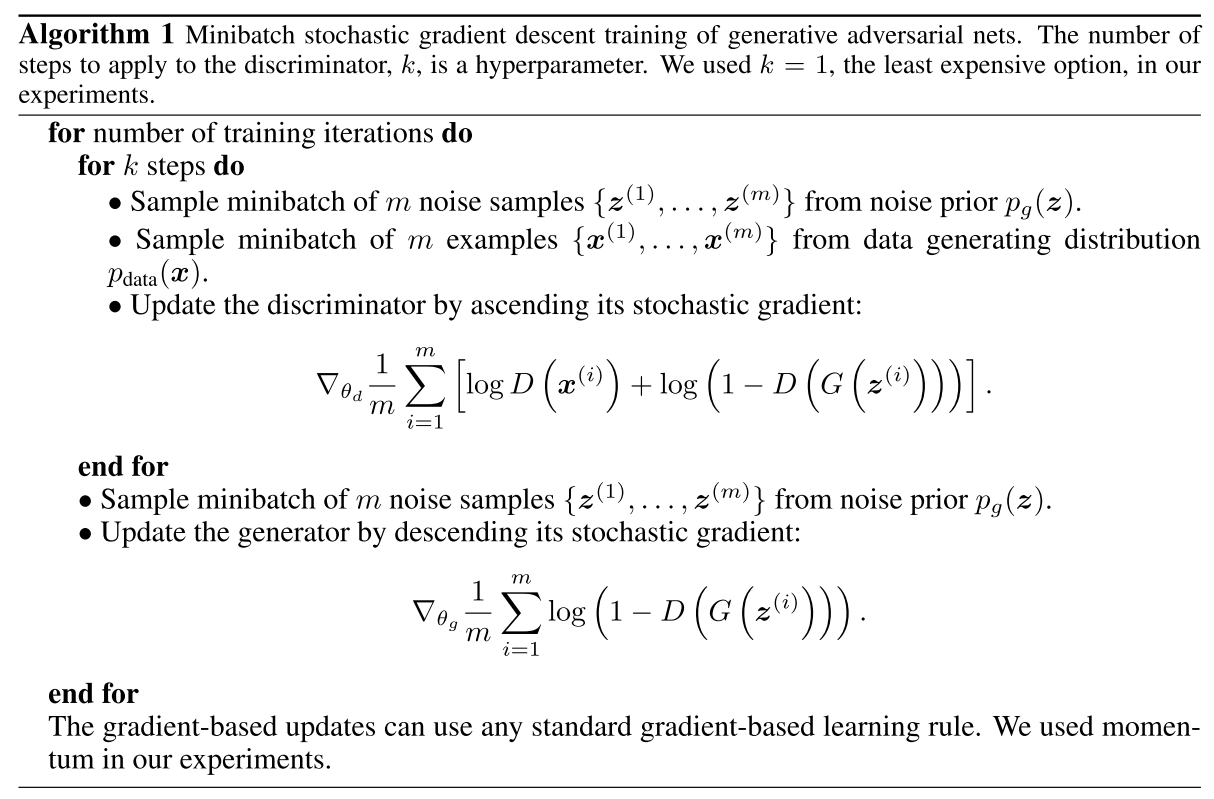
\includegraphics[scale=0.3]{./images/generative/gan/gan_algorithm.png}
	\caption{Training GAN}
	\label{fig:algorithm}
\end{figure}

\section{Some notes}
What would be the optimal discriminator that separates the two different distributions $p(x)$ and $q(x)$? It turns out that it is
$$f(x) = \frac{q(x)}{p(x)+q(x)}$$
Actually, there are many choices for classifiers e.g., KL-divergence

\begin{enumerate}
	\item What do we need to learn a classifier?
	\begin{itemize}
		\item Only samples from $p(x)$ and $q(x)$
	\end{itemize}
	\item How do we parameterize $q(x)$?
	\begin{itemize}
		\item Parametric density function (Gaussian)
		\item Define implicitly (GANs approach): define mapping from one (noise) to another (data or image)
	\end{itemize}
\end{enumerate}

The orignal GAN does not learn the data distributions. 





\section{Wasserstein Generative Adversarial Networks}
\subsection{KL Divergence}
Definition:
$$D_\textrm{KL}(q(x)||p(x)) = \int q(x)\log \frac{q(x)}{p(x)}dx$$
\begin{itemize}
	\item Forward KL: 
	\begin{itemize}
		\item If $q(z)\rightarrow 0, \textrm{Forward KL}\rightarrow \infty$ 
		\item Zero avoiding for $q(z)$ 
	\end{itemize}
	\item Reverse KL:
	\begin{itemize}
		\item If $p(z)\rightarrow 0, \textrm{Reverse KL}\rightarrow \infty$ 
		\item Zero forcing: $q(z)\rightarrow 0$ 
	\end{itemize}
\end{itemize}

Typically, $p(x)$ and $q(x)$ are far apart at the initial state. 

\begin{figure}[h]
	\begin{center}
		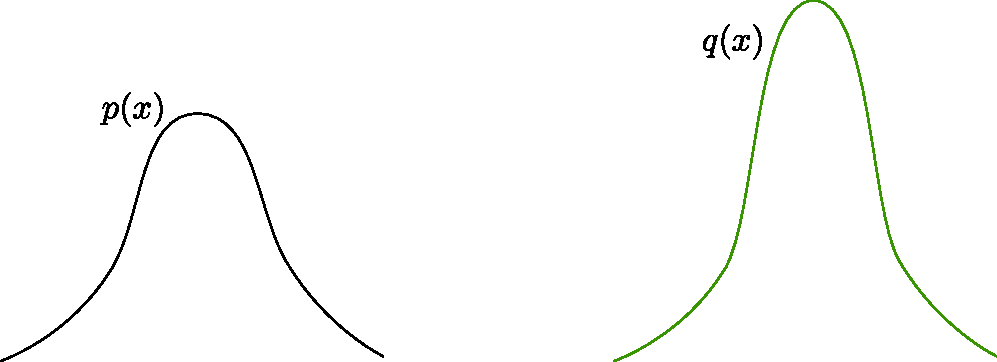
\includegraphics[scale=0.5]{./images/generative/gan/twodist.pdf}
	\end{center}
	\caption{Two distributions: $p(x)$ and $q(x)$}
	\label{fig:}
\end{figure}

Thus, both the forward KL and the reverse KL suffers an unstability issue. Specifically, in each case, if the denominator goes to zero, then the divergence goes to infinity. 

\subsection{Jensen-Shannon Divergence}

Definition:
$$D_{JS}(p_{data}||p_{G}) = \frac{1}{2}\Bigg[D_{KL}\Big(p_{data}\Big|\Big|\frac{p_{data}+p_{G}}{2}\Big)+D_{KL}\Big(p_{G}\Big|\Big|\frac{p_{data}+p_{G}}{2}\Big)\Bigg]$$

The KL divergence's issue can be alleviated by JS-divergence. Consider a simple example in Fig. \ref{fig:wassersteinexample}6
\begin{align*}
	\forall (x, y) \in P, x = 0 \text{ and } y \sim U(0, 1)\\
	\forall (x, y) \in Q, x = \theta, 0 \leq \theta \leq 1 \text{ and } y \sim U(0, 1)
\end{align*}

\begin{figure}[h]
	\begin{center}
		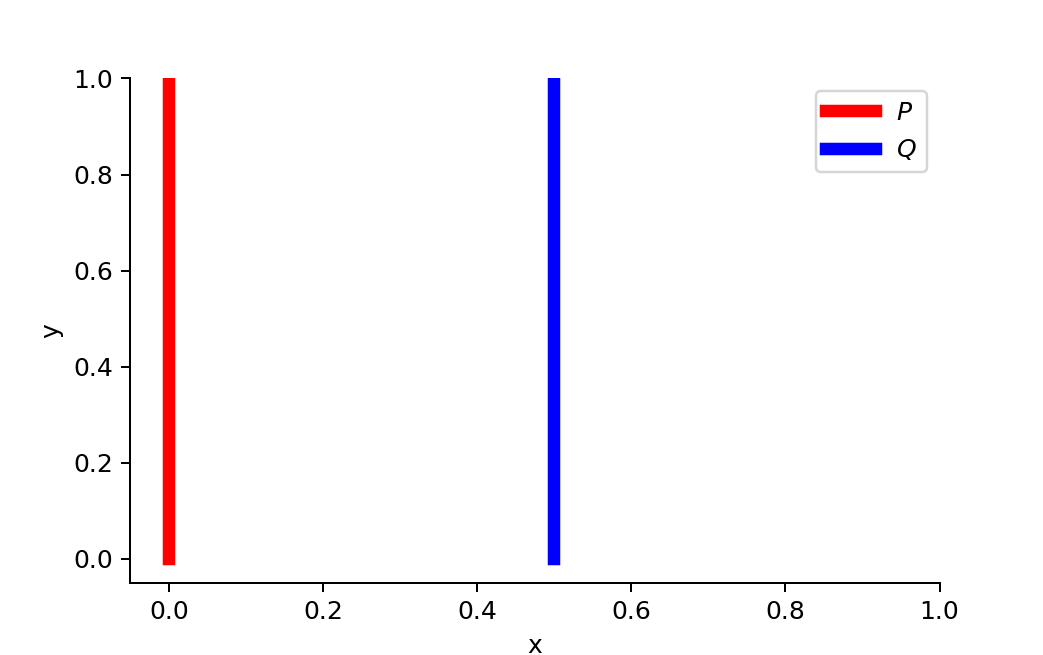
\includegraphics[scale=0.25]{./images/generative/gan/wassersteinexample.png}
	\end{center}
	\caption{Two distributions: $p(x)$ and $q(x)$}
	\label{fig:wassersteinexample}
\end{figure}

\begin{align*}
	D_\textrm{KL}(q(x)||p(x)) &= \infty\\
	D_\textrm{KL}(p(x)||q(x)) &= \infty\\
	D_{JS}(p_{data}||p_{G}) &= \frac{1}{2}\Bigg[D_{KL}\Big(p_{data}\Big|\Big|\frac{p_{data}+p_{G}}{2}\Big)+D_{KL}\Big(p_{G}\Big|\Big|\frac{p_{data}+p_{G}}{2}\Big)\Bigg]\\
	& = \frac{1}{2}\Bigg[D_{KL}\Big(p_{data}\Big|\Big|\frac{p_{data}}{2}\Big)++D_{KL}\Big(p_{G}\Big|\Big|\frac{p_{G}}{2}\Big)\Bigg]\\
	& = \frac{1}{2}[\log 2 + \log 2] = \log 2\\
	W(p,q) & = |\theta|
\end{align*}
Therefore, Jensen-Shannon divergence is more stabler than KL divergece. This is one of the reasons why GAN, which uses JS divergence works better than VAE, which uses KL divergence. 

However, JS divergence also has some problem. If the value is close to $\frac{1}{2}\log 2$, then the gradient will be very small or close to zero, because the divergence is close to constant. It means that a training speed is very slow. Thus, we need a better metric. 

\subsection{Wasserstein Distance}
Wasserstein Distance is a measure of the distance between two probability distributions. It is also called Earth Mover’s distance, short for EM distance, because informally it can be interpreted as the minimum energy cost of moving and transforming a pile of dirt in the shape of one probability distribution to the shape of the other distribution.
\begin{equation*}
	W(p_r, p_g) = \inf_{\gamma \sim \Pi(p_r, p_g)} \mathbbm{E}_{(x, y) \sim \gamma}[\| x-y \|]
\end{equation*}

\begin{itemize}
	\item $\Pi$: is the transportation plan and the set of all possible joint probability distributions between $p_r$ and $p_g$. One joint distribution $\gamma \sim \Pi(p_r, p_g)$ describes one transport plan.\
	\item $\mathbbm{E}_{x, y \sim \gamma} \| x-y \| = \sum_{x, y} \gamma(x, y) \| x-y \|$
	\item Finally, we take the minimum one among the costs of all dirt moving solutions as the EM distance (by infimum). 
\end{itemize}

\section{WGAN}
However, consider all possible joint distribution is intractable, so dual solution can be used. 

$$W(p_r, p_g) = \frac{1}{K} \sup_{\| f \|_L \leq K} \mathbbm{E}_{x \sim p_r}[f(x)] - \mathbbm{E}_{x \sim p_g}[f(x)]$$

So to calculate the Wasserstein distance, we just need to find a 1-Lipschitz function. To enforce the constraint, WGAN applies a very simple clipping to restrict the maximum weight value in $f$, i.e. the weights of the discriminator

Suppose this function $f$ comes from a family of $K$-Lipschitz continuous functions, $\{f_w\}_{w\in W}$, parameterized by $w$. In the modified Wasserstein-GAN, the ``discriminator'' model is used to learn $w$ to find a good $f_w$ and the loss function is configured as measuring the Wasserstein distance between $p_r$ and $p_g$.

$$L(p_r, p_g) = W(p_r, p_g) = \max_{w \in W} \mathbbm{E}_{x \sim p_r}[f_w(x)] - \mathbbm{E}_{z \sim p_r(z)}[f_w(g_\theta(z))]$$

There are two ways to satisfy the Lipschitz continuity:
\begin{itemize}
	\item Weight clipping
	\item Gradient Penalty
\end{itemize}

\subsection{Lipschitz continuity}
The function $f$ in the new form of Wasserstein metric is demanded to satisfy $\| f \|_L \leq K$, meaning it should be $K$-Lipschitz continuous. \citep{Lil2017}

A real-valued function $f: \mathbbm{R} \rightarrow \mathbbm{R}$ is called $K$-Lipschitz continuous if there exists a real constant $K\geq 0$ such that, for all $x_1, x_2 \in \mathbbm{R}$
$$\lvert f(x_1) - f(x_2) \rvert \leq K \lvert x_1 - x_2 \rvert$$
Here $K$ is known as a Lipschitz constant for function $f(\cdot)$. Functions that are everywhere continuously differentiable is Lipschitz continuous, because the derivative, estimated as $\frac{\lvert f(x_1) - f(x_2) \rvert}{\lvert x_1 - x_2 \rvert}$, has bounds. However, a Lipschitz continuous function may not be everywhere differentiable, such as $f(x) = \lvert x \rvert$

\begin{figure}[h]
	\begin{center}
		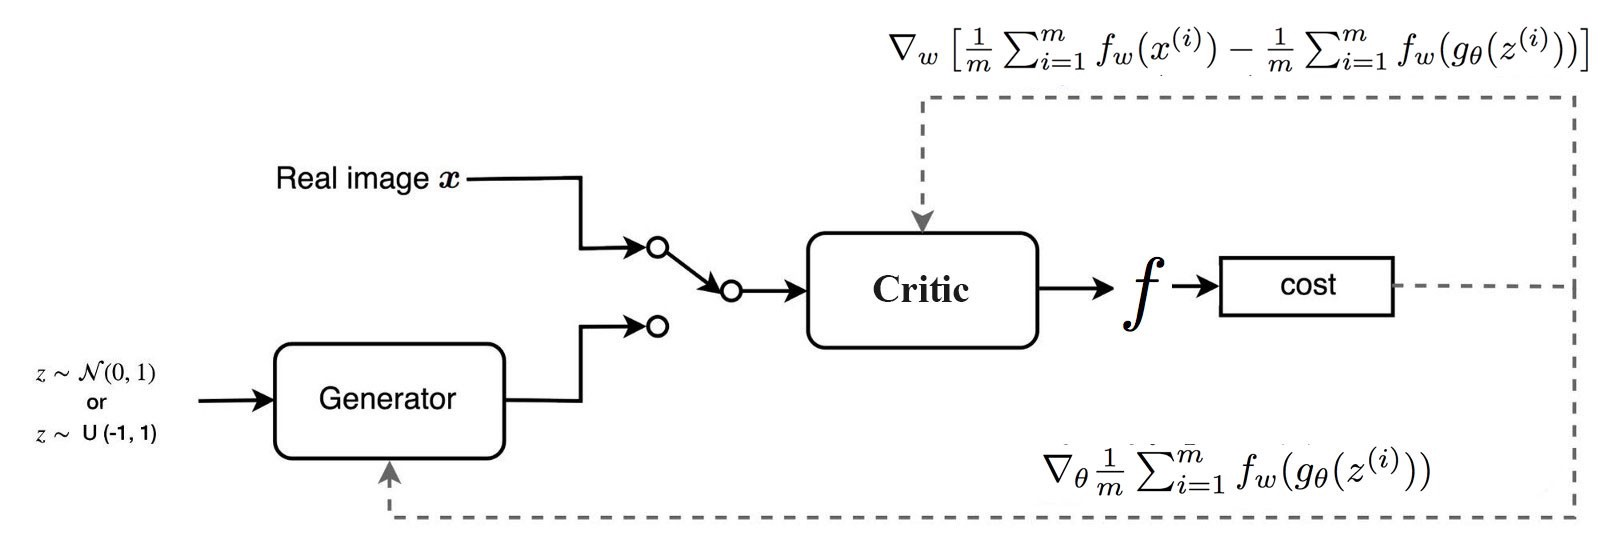
\includegraphics[scale=0.25]{./images/generative/gan/wgan.jpeg}
	\end{center}
	\caption{WGAN}
	\label{fig:wgan}
\end{figure}

\begin{figure}[h]
	\begin{center}
		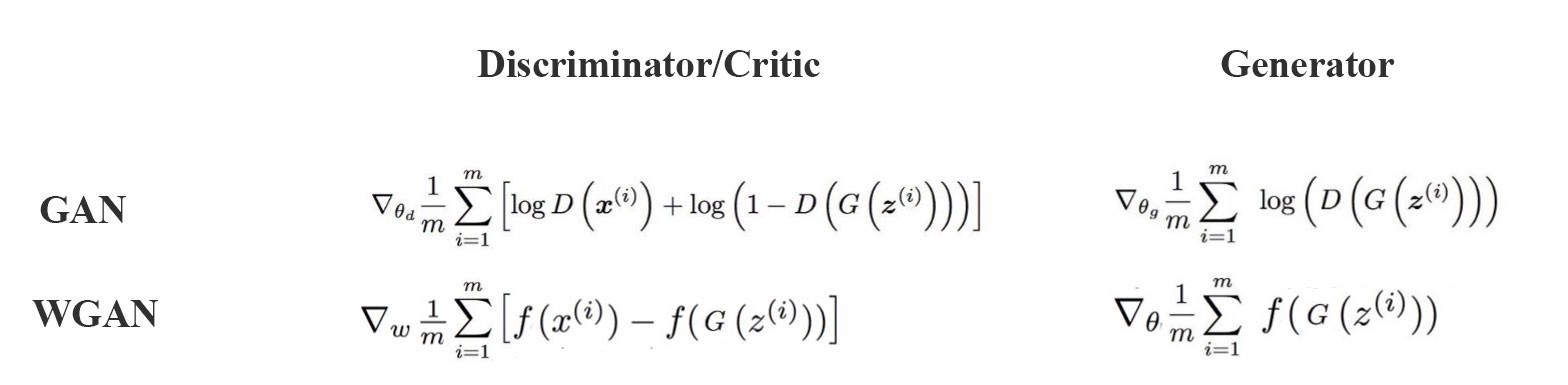
\includegraphics[scale=0.2]{./images/generative/gan/wgan_2.jpeg}
	\end{center}
	\caption{WGAN}
\end{figure}

\section{InfoGAN: Interpretable Representation Learning by Information Maximizing Generative Adversarial Nets}
\label{sec:q}

\subsection{Joint Entropy}
\begin{align*}
H(X,Y) = \mathbb{E}_{X,Y}[-\log p(x,y)] = -\sum_{x,y}p(x,y)\log p(x,y)
\end{align*}
\subsection{Conditional Entropy}
\begin{align*}
H(X|Y) &= \mathbb{E}_{Y}[H(X,Y)] \\
&= -\sum_{y\sim p_Y(y)}p(y)\sum_{x\sim p_X(x)}p(x|y)\log p(x|y)\\
& = -\sum_{y\sim p_Y(y)}\sum_{x\sim p_X(x)}p(y)p(x|y)\log p(x|y)\\
& = -\sum_{y\sim p_Y(y)}\sum_{x\sim p_X(x)}p(x,y)\log p(x|y) = -\mathbb{E}_{x,y}[\log p(x|y)]\\
& = -\sum_{y\sim p_Y(y)}\sum_{x\sim p_X(x)}p(x,y)\log \frac{p(x,y)}{p(y)}\\
& = -\sum_{y\sim p_Y(y)}\sum_{x\sim p_X(x)}p(x,y)\log p(x,y) + \sum_{y\sim p_Y(y)}\sum_{x\sim p_X(x)}p(x,y)\log p(y)\\
& = H(X,Y) - H(Y)
\end{align*}
\subsection{Variational Mutual Information Maximization}
\begin{align*}
I(c;G(z,c)) &= H(c) - H(c|G(z,c))\\
& = H(c) + \int\int p(c=c',x=G(z,c))\log p(c=c'|x=G(z,c)) dc' dz\\
& = H(c) + \mathbb{E}_{x\sim G(z,c),c'\sim p(c|x)}[\log p(c'|x)]\\
& = H(c) + \mathbb{E}_{x\sim G(z,c)}\mathbb{E}_{c'\sim p(c|x)}[\log p(c'|x)]\\
& = H(c) + \mathbb{E}_{x\sim G(z,c)}\mathbb{E}_{c'\sim p(c|x)}\Bigg[\log \frac{p(c'|x)Q(c'|x)}{Q(c'|x)}\Bigg]\\
& = H(c) + \mathbb{E}_{x\sim G(z,c)}\mathbb{E}_{c'\sim p(c|x)}\Bigg[\log \frac{p(c'|x)}{Q(c'|x)}\Bigg] + \mathbb{E}_{x\sim G(z,c)}\mathbb{E}_{c'\sim p(c|x)}\Big[\log Q(c'|x)\Big]\\
& = H(c) + \mathbb{E}_{x\sim G(z,c)}\Bigg[D_{KL}(p(c'|x)||Q(c'|x))\Bigg] + \mathbb{E}_{x\sim G(z,c)}\mathbb{E}_{c'\sim p(c|x)}\Big[\log Q(c'|x)\Big]\\
& \geq H(c) + \mathbb{E}_{x\sim G(z,c)}\mathbb{E}_{c'\sim p(c|x)}\Big[\log Q(c'|x)\Big] \footnotemark
\end{align*}

Thus we get a lower bound for the mutual information as follows:

$$I(c;G(z,c)) \geq H(c) + \mathbb{E}_{x\sim G(z,c)}\mathbb{E}_{c'\sim p(c|x)}\Big[\log Q(c'|x)\Big]$$

However, we still have a problem. We need to sample $c$ from $p(c|x)$. Thus, we need to replace it with a known distribution. Firstly, with the reasoning that $x\sim G(z,c)$ means sample $c$ from $p(c)$ then sample $x$ from $G(z,c)$. So we can express $\mathbb{E}_{x\sim G(z,c)}$ with $\mathbb{E}_{c\sim p(c)}\mathbb{E}_{x\sim G(z,c)}$. and by the Lemma \ref{lemma:1}, 
\begin{align*}
I(c;G(z,c)) &\geq H(c) + \mathbb{E}_{x\sim G(z,c)}\mathbb{E}_{c'\sim p(c|x)}\Big[\log Q(c'|x)\Big]\\
&= H(c) + \mathbb{E}_{c\sim p(c)}\mathbb{E}_{x\sim G(z,c)}\mathbb{E}_{c'\sim p(c|x)}\Big[\log Q(c'|x)\Big]\\
& = H(c) + \mathbb{E}_{c\sim p(c)}\mathbb{E}_{x\sim G(z,c)}\Big[\log Q(c'|x)\Big] \footnotemark
\end{align*}

Thus, we can directly sample $c$ from the known distribution instead of $p(c|x)$.

\begin{lemma}
	For random variables $X, Y$ and function $f(x, y)$ under suitable regularity conditions:
	$$\mathbb{E}_{x\sim X, y\sim Y|x}[f(x,y)] = \mathbb{E}_{x\sim X, y\sim Y|x, x'\sim X|y}[f(x',y)]$$
	\begin{proof}
		\begin{align*}
		\mathbb{E}_{x\sim X, y\sim Y|x}[f(x,y)] &=\int_x P(x)\int_y P(y|x)f(x,y)dydx\\
		& = \int_x\int_yP(x,y)f(x,y)dydx\\
		& = \int_{x'}\int_yP(x',y)f(x',y)dydx'\\
		& = \int_{x'}\int_y P(y)P(x'|y)f(x',y)dydx'\\
		& = \int_{x'}\int_y\int_{x} P(x,y)P(x'|y)f(x',y)dxdydx'\\
		& = \int_{x}P(x)\int_y P(x|y) \int_{x'} P(x'|y)f(x',y)dxdydx'\\
		& = \mathbb{E}_{x\sim X, y\sim Y|x, x'\sim X|y}[f(x',y)]
		\end{align*}
	\end{proof}
	\label{lemma:1}
\end{lemma} 


% \chapter{Introduction}
\section{Introduction}
The HMM is based on the Markov chain assumption. A Markov chain is a model
that tells us something about the probabilities of sequences of random variables,
states, each of which can take on values from some set. These sets can be words, or
tags, or symbols representing anything, like the weather.

There are two important assumptions:
\begin{itemize}
	\item Markov assumption
	\item Output independence: $p(x_i|z_1,\dots,z_i,\dots,z_T,x_1,\dots,x_i,\dots,x_T) = p(x_i|z_i)$
\end{itemize}

\subsection{Conditional Independence}
If two events $A$ and $B$ are \textbf{conditionally independent} given an event $C$ then,
\begin{itemize}
	\item $P(A\cap B|C) = P(A|C)P(B|C)$. 
	\item $P(A|B,C) = P(A|C)$
\end{itemize}

\subsection{Notation}

\begin{itemize}
	\item $X = (x_i, x_2,\dots, x_T)$
	% \item $x_i\in\{c_1,...,c_m\}$
	\item Initial state probabilities: $p(z_1) \sim \textrm{Multinomial}(\pi_1,...,\pi_k)$, need to learn $\pi$
	\item Transition probability:
	$$p(z_t|z_{t-1}=i)\sim \textrm{Multinomial}(a_{i,1},...,a_{i,k})$$
	, where $a_{i,j} = p(z_t=j|z_{t-1}=i)$ and $i$ and $j$ denote clusters or states, respectively.
	\item Emission probability:
	$$p(x_t|z_{t}=i)\sim \textrm{Multinomial}(b_{i,1},...,b_{i,m})$$
	, where $b_{i,j} = p(x_t=j|z_{t}=i)$
\end{itemize}


\section{Bayesian Network}
\subsection{Bayes Ball}

\begin{figure}[h!]
	\centering
	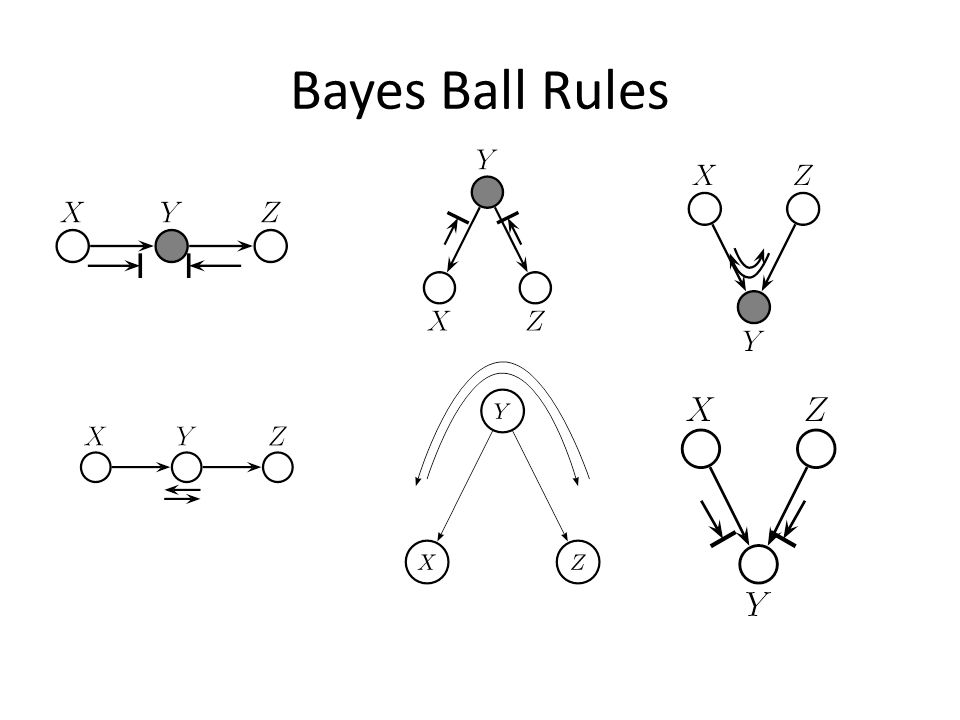
\includegraphics[scale=0.3]{./images/hmm/bayes.jpg}
	\caption{Bayes ball}
	\label{fig:bayes}
\end{figure}

\begin{itemize}
	\item Cascading: $P(Z|Y,X) = P(Z|Y)$. The information of $Y$ decouples $X$ and $Z$.
	\item Common parent: $P(X,Z|Y) = P(X|Y)P(Z|Y)$. The information of $Y$ decouples $X$ and $Z$.
	\item V-Structure (common child): Unlike the above two cases, the information of $Y$ couples $X$ and $Z$.
		$$P(X,Y,Z) = P(X)P(Y)P(Y|X,Z).$$
\end{itemize}

\subsection{Potential Function}
Potential function is a function which is not a probability function, but it can become a probability function by normalizing it. 
$$P(A,B,C,D) = P(A|B)P(B|C)P(C|D)P(D)$$

\begin{figure}[h]
	\centering
	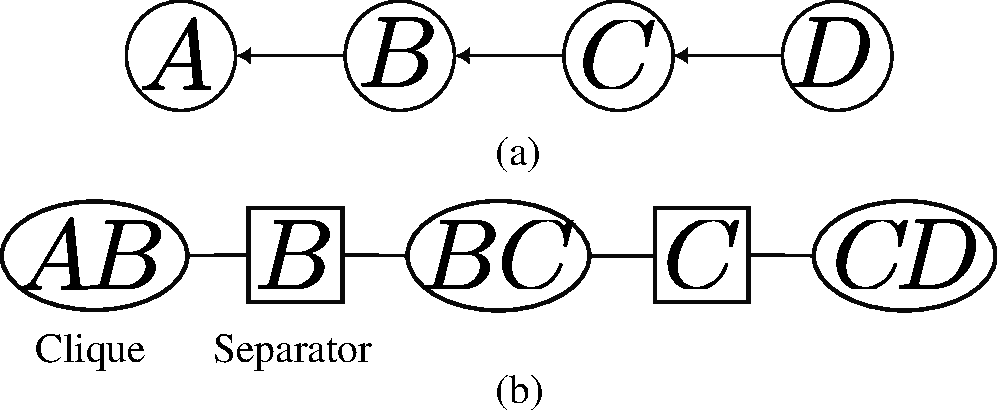
\includegraphics[scale=0.5]{./images/hmm/cascade.pdf}
\end{figure}

\begin{itemize}
	\item Cliques: $\Psi(a,b), \Psi(b,c), \Psi(c,d)$
	\item Separators $\phi(b), \phi(c)$
\end{itemize}
Given a clique tree with cliques and separators, the joint probability distribution is defined as follows:
% By using potential functions, we can express the joint probability as
\begin{align*}
	P(A,B,C,D) &= P(U) = \frac{\prod_N \Psi(N)}{\prod_L\phi(L)}= \frac{ \Psi(a,b)\Psi(b,c)\Psi(c,d)}{\phi(b)\phi(c)}\\
\end{align*}
An effect of an observation propagates through the clique graph $\to$ \textbf{Belief propagation}. How to propagate the belief? \textbf{Absorption rule}!

Let's say we have some new observations about $A$, then it affects the clique $\Psi(a,b)$. The updated clique is now $\Psi^*(a,b)$. Similarly, $\phi^*(b) = \sum_A\Psi^*(a,b)$. Subsequently, $\Psi^*(b,c) = \Psi^(b,c)\frac{\phi^*(b)}{\phi(b)}$.



\chapter{Hidden Markov Model}
\begin{figure}[h]
	\begin{center}
		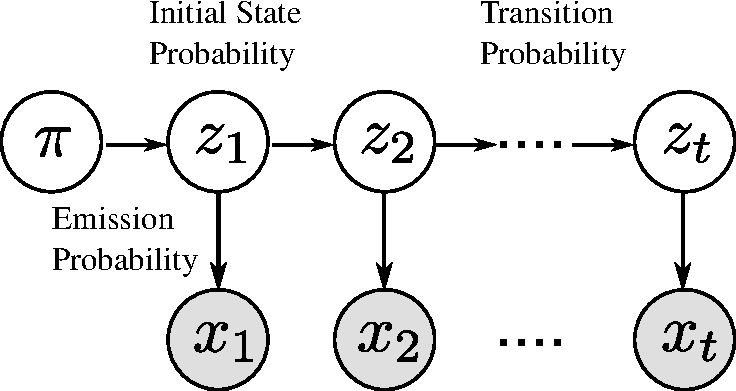
\includegraphics[scale=0.7]{./images/hmm/hmm_figure.pdf}
	\end{center}
	\caption{HMM Structure}
	\label{fig:HMM}
\end{figure}

The observation can be discrete or continuous. If the latent factors are continuous, then HMM is often referred as \textbf{Kalman filter}. 

\begin{itemize}
	\item Initial state probability: $P(z_1)\sim \textrm{Mult}(\pi_1, \dots, \pi_k)$
	\item Transition probability: $P(z_t|z^i_{t-1}=1)\sim \textrm{Mult}(a_{i,1}, \dots, a_{i,k})$, \\ where $P(z_t^j=1|z_{t-1}^i=1) = a_{i,j}$
	\item Emission probability: $P(x_t|z_t^i=1)\sim \textrm{Mult}(b_{i,1}, \dots, b_{i,m})\sim f(x_t|\theta_i)$,\\ where $P(x_t^j=1|z_{t}^i=1) = b_{i,j}$. The probability of observing $x_j$ at the  $i$-th cluster. 
\end{itemize}
Note that $i$ and $j$ are indices of clusters. 

There are three main problems in HMM:
\begin{enumerate}
	\item Evaluation Questions (likelihood): %Forward algorithm
	\begin{itemize}
		\item Given $\boldsymbol{\pi}\mathbf{, a, b}, X$
		\item Find $p(X|M, \boldsymbol{\pi}\mathbf{, a, b})$
		\item How much are $X$ likely to be observed by a model $M$?
	\end{itemize}
	
	\item Decoding Questions:
	\begin{itemize}
		\item Given $\boldsymbol{\pi}\mathbf{, a, b}, X$
		\item Find $\argmax_Z p(Z|X, M, \boldsymbol{\pi}\mathbf{, a, b})$
		\item What is the most probable sequence of $Z$ (latent states)? 
	\end{itemize}
	
	\item Learning Questions: Forward-Backward (Baum-Welch)
	\begin{itemize}
		\item Given $X$
		\item Find $\argmax_{\boldsymbol{\pi}\mathbf{, a, b}} p(X|M, \boldsymbol{\pi}\mathbf{, a, b})$
		\item What would be the optimal model parameters? 
	\end{itemize}
\end{enumerate}

% For a given hidden state, we can easily compute the output likelihood.

\section{Evaluation: Forward-Backward Probability}
% The forward–backward algorithm is an inference algorithm for hidden Markov models which computes the posterior marginals of all hidden state variables given a sequence of observations/emissions

% The term forward–backward algorithm is also used to refer to any algorithm belonging to the general class of algorithms that operate on sequence models in a forward–backward manner.

% In the first pass, the forward–backward algorithm computes a set of forward probabilities which provide, for all $t\in \{1,\dots ,T\}$, the probability of ending up in any particular state given the first $t$ observations in the sequence, i.e. $P(X_{t}\ |\ o_{1:t})$. In the second pass, the algorithm computes a set of backward probabilities which provide the probability of observing the remaining observations given any starting point $t$, i.e. $P(o_{t+1:T}\ |\ X_{t})$. These two sets of probability distributions can then be combined to obtain the distribution over states at any specific point in time given the entire observation sequence:

% These two sets of probability distributions can then be combined to obtain the distribution over states at any specific point in time given the entire observation sequence:
% $$P(X_{t}\ |\ o_{1:T})=P(X_{t}\ |\ o_{1:t},o_{t+1:T})\propto P(o_{t+1:T}\ |\ X_{t})P(X_{t}|o_{1:t})$$
% The forward–backward algorithm can be used to find the most likely state for any point in time. However, It cannot be used to find the most likely sequence of states.

\subsection{Joint Probability}
We can factorize the joint distribution of HMM in \Cref{fig:HMM} by using a Bayesian approach as follows:. 

\begin{align}
	p(X,Z) = p(x_1,\dots,x_t, z_1,\dots,z_t) = p(z_1)p(x_1|z_1),p(z_2|z_1),\dots,p(x_{t}|z_{t}),p(z_{t}|z_{t-1})
	\label{eq:hmm_joint}
\end{align}

As the number of latent factor increases, it is getting harder to decode the latent factors. 

\subsection{Marginal Probability}
% \subsection{Forward Probability}
We want to compute the likelihood of sequence $X$ which is given by
$$p(X|\boldsymbol{\pi}\mathbf{, a, b}) = \sum_Z p(X, Z|\boldsymbol{\pi}\mathbf{, a, b})$$
The computation can be done as follows:
\begin{align*}
	p(X) &= \sum_Z p(X,Z)\\
	& = \sum_{z_1}\dots\sum_{z_t}p(x_1,\dots,x_t,z_1,\dots,z_t)\\
	& = \sum_{z_1}\dots\sum_{z_t}\pi_{z_{1}}\prod_{t=2}^{T}a_{z_{t-1},z_t}\prod_{t=1}^{T}b_{z_{t},x_t}
\end{align*}
The last step is done by using \Cref{eq:hmm_joint}). The computation of this equation requires lots of computations, so we will change it into a \textbf{recursive form} by using the factorization rule $p(a,b,c) = p(a)p(b|a)p(c|a,b)$. 

\begin{align}
	p(&x_1,\dots,x_t,z_t^k=1) = \sum_{z_{t-1}}p(x_1,\dots,x_{t-1}, x_t,z_{t-1},z_t^k=1)\\
	&= \sum_{z_{t-1}} p(\underbrace{x_1,\dots,x_{t-1}, z_{t-1}}_{a}, \underbrace{x_t}_{c}, \underbrace{z_t^k=1}_{b})\\
	& = \sum_{z_{t-1}} p(x_1,\dots,x_{t-1},z_{t-1}) p(z_t^k=1|x_1,\dots,x_{t-1},z_{t-1})p(x_t|z_t^k=1, x_1,\dots,x_{t-1},z_{t-1}) \\
	&\hspace{0.5cm} \because p(a,b,c) = p(a)p(b|a)p(c|a,b) \textrm{ or by the structure of HMM}\nonumber\\ 
	& = \sum_{z_{t-1}} p(x_1,\dots,x_{t-1},z_{t-1}) p(z_t^k=1|z_{t-1}) p(x_t|z_t^k=1)\\
	& = p(x_t|z_t^k=1) \sum_{z_{t-1}} p(x_1,\dots,x_{t-1},z_{t-1}) p(z_t^k=1|z_{t-1}) \\
	& = b_{z^k_t,x_t} \sum_{z_{t-1}} p(x_1,\dots,x_{t-1},z_{t-1}) a_{z_{t-1},z_t^k}
	\label{eq:hmm_eval_fact}
\end{align}

\begin{itemize}
	\item In the second line, the $x_{t-1}$ and $z_{t-1}$ are grouped together. 
	\item Then, we can find the HMM structure by factorizing the equation. 
	\item In the fourth line, $x$ terms are removed, since $z_t$ only relies on $z_{t-1}$ by the Markov assumption. Similarly, $x_t$ only depends on $z_t$. We can interpret this by using Bayes ball too. 
\end{itemize}
% In the fifth step, we assume that $z_t=k$ is given, thus by Markov assumption, we only need $z_{t-1}$. 
Now we can find a recursive structure of $p(x_1,\dots,x_{t},z_{t}^k=1)$ as follows:
$$\alpha_t^k = p(x_1,\dots,x_{t},z_{t}^k=1) = b_{k,x_t}\sum_i \alpha_{t-1}^ia_{i,k}$$
, where \textbf{$\alpha_t^k$ is the probabilities of being in state $k$ after observing the first $t$ observations.} Thus, 
\begin{align*}
	p(x_1,\dots,x_{t}) & = \sum_{\mathbf{z}} p(x_1,\dots,x_{t},z)\\
	& = \sum_{k} \alpha_t^k
\end{align*}
% \begin{itemize}
% 	\item $\alpha_t^k$: \textbf{Forward probability}. Probabilities of being in state $k$ after observing the first $t$ observations.
% 	% \item $a_{i,k}$: transition probability
% 	% \item $b_{k,x_t}$: observation (or emission) probability
% \end{itemize}
Note that $\alpha_t^k$ is also called \textbf{Forward probability}.

\subsection{Forward Algorithm}
Forward probability solves the evaluation problem. Essentially, this is a dynamic programming, so it calculates required values in a bottom-up manner. 
\begin{itemize}
	\item Forward probability: $\alpha_t^k$, $Time\times States$
\end{itemize}
%\LinesNumbered
\begin{algorithm}
	Create a probability matrix $forward[M,T] = \alpha_t^k$\\
	Initialization: \\
	\For {\textrm{each state} k=1,...,M}{
		$\alpha_1^k\leftarrow \pi_kb_{k,x_1}$
	}
	\For {\textrm{time step} t=2,...,T}{
		\For {\textrm{each step} k=1,...,M}{
			$\alpha_t^k = b_{k,x_t}\sum_i \alpha_{t-1}^ia_{i,k}$
			}
		
	}
	Return $p(X) = \sum_i^M \alpha_T^i$
	\caption{Forward Algorithm}
	\label{algo:forward_algorithm}
\end{algorithm}
%\begin{algorithm}
%	Init: $\alpha_1^k = b_{k,x_1}\pi_k$\\
%	\For{t=1,...,T}{
%		$\alpha_t^k = b_{k,x_t}\sum_i \alpha_{t-1}^ia_{i,k}$
%	}
%	Return $p(X) = \sum_i\alpha_T^i$
%	\caption{Forward Algorithm}
%	\label{algo:forward_algorithm}
%\end{algorithm}
Note again that 
$$p(X) = p(x_1,...,x_T) =\sum_i\alpha_T^i = \sum_i p(x_1,...,x_T, z_T^i=1)$$
Note also that the forward-algorithm returns $p(X)$ and forward probability is the probability of being in state $k$ after observing the first $t$ observations without $Z$. 

\subsection{Backward Probability}
The forward probability only considers an observation at $t$. To determine the $z_t$, we need to leverage the future observations. \textbf{The backward probability $\beta$ is the probability of seeing the observations from time $t+i$ to the end, given that we are in state $k$ at time $t$.} 
$$\beta_t^k = p(x_{t+1},\dots,x_T|z_t^k=1)$$
We want to compute $p(z_t^k=1|X)$ rather than $p(x_1,\dots,x_t, z_t^k=1)$. In other words, we will leverage the whole observations $X$. 
\begin{align*}
	p(z_t^k=1,X) &= p(x_1,\dots,x_t, z_t^k=1, x_{t+1},\dots,x_T)\\
	& = p(x_1,\dots,x_t, z_t^k=1)p(x_{t+1},\dots,x_T|x_1,\dots,x_t, z_t^k=1)\\
	& = p(x_1,\dots,x_t, z_t^k=1)p(x_{t+1},\dots,x_T|z_t^k=1)\\
	& = \alpha_{t}^k\beta_{t}^k
\end{align*}
We already know that $p(x_1,\dots,x_t, z_t^k=1) = \alpha_t^k$. We just need to compute backward probability as follows:
\begin{align*}
	\beta_t^k &= p(x_{t+1},\dots,x_T|z_t^k=1)\\
	& = \sum_{z_{t+1}}p(\underbrace{z_{t+1}}_{a}, \underbrace{x_{t+1}}_b,\underbrace{x_{t+2},\dots,x_T}_c|z_t^k=1)\\
	& = \sum_{i} p(z_{t+1}^i=1|z_t^k=1)p(x_{t+1}|z_{t+1}^i=1,z_t^k=1)p(x_{t+2},\dots,x_T|x_{t+1},z_{t+1}^i=1,z_t^k=1)\\
	& \because p(a,b,c) = p(a)p(b|a)p(c|a,b)\\
	& = \sum_{i} p(z_{t+1}^i=1|z_t^k=1)p(x_{t+1}|z_{t+1}^i=1)p(x_{t+2},\dots,x_T|z_{t+1}^i=1)\\
	& = \sum_{i}a_{k,i}b_{i,x_{t+1}} \beta_{t+1}^i
\end{align*}

Another recursive structure:
\begin{align*}
	p(z_t^k=1,X) &= \alpha_{t}^k\beta_{t}^k\\
	& = b_{k,x_t}\sum_i \alpha_{t-1}^ia_{i,k} \times \sum_{i}a_{k,i}b_{i,x_{t}} \beta_{t+1}^i
\end{align*}
This means at time $t$, the latent label is belong to some class $k$ and this can be computed by using the forward probability and the backward probability. Now we can compute
\begin{align*}
p(z_t^k=1|X) &= \frac{p(z_t^k=1,X)}{p(X)} = \frac{\alpha_{t}^k\beta_{t}^k}{p(X)}
\end{align*}
Then, 
$$k_t = \argmax_{k}p(z_t^k=1|X)$$
Note that this is for a single latent variable at a single time step given the whole observation $X$, but we want to decode a sequence of latent variables. Thus, we need some decoding algorithm.

\section{Decoding: Viterbi Algorithm}
For any model, such as an HMM, that contains hidden variables, \textbf{the task of determining which sequence of variables is the underlying source of some sequence of observations is called the decoding task}.

We might propose to find the best sequence as follows: 
\begin{enumerate}
	\item For each possible hidden state sequence (HHH, HHC, HCH, etc.), we could run the forward algorithm and compute the likelihood of the observation sequence given that hidden state sequence.
	\item Then, we could choose the hidden state sequence with the maximum observation likelihood.
\end{enumerate}  
However, this is not a feasible solution, because there are an exponentially large number of state sequences.

Instead, the most common decoding algorithms for HMMs is the \textbf{Viterbi algorithm}. Like the forward algorithm, \textbf{Viterbi} is a kind of \textbf{dynamic programming algorithm.}

Note that the Viterbi algorithm is identical to the forward algorithm except that it takes the \textbf{max} over the previous path probabilities whereas the forward algorithm takes the \textbf{sum}. This is because, we want to obtain \textbf{the most probable latent variable sequence}. Note also that the Viterbi algorithm has one component that the forward algorithm doesn't have: \textbf{backpointers}. The reason is that while the forward algorithm needs to produce an observation likelihood, the Viterbi algorithm must produce a probability and also the most likely state sequence. We compute this best state sequence by keeping track of the path of hidden states that led to each state and then at the end backtracing the best path to the beginning (the Viterbi backtrace).

We can leverage the forward-backward probabilities:
\begin{itemize}
	\item $k^* = \argmax_{k}p(z_t^k=1|X) = \argmax_{k}p(z^k_t=1,X) = \argmax_{k}\alpha_{t}^k\beta_{t}^k$
\end{itemize}
We will use a forward approach:
% \setcounter{equation}{0}
\begin{align}
	V_t^k &= \max_{z_1,\dots,z_{t-1}}p(x_1,\dots,x_{t-1},z_1,\dots,z_{t-1},x_t,z_t^k=1)\\ 
	& = \max_{z_1,\dots,z_{t-1}}p(x_t,z_t^k=1|x_1,\dots,x_{t-1},z_1,\dots,z_{t-1})p(x_1,\dots,x_{t-1},z_1,\dots,z_{t-1})\\
	& = \max_{z_1,\dots,z_{t-1}}p(x_t,z_t^k=1|z_{t-1})p(x_1,\dots,x_{t-2},z_1,\dots,z_{t-2}, x_{t-1}, z_{t-1})\\
	& = \max_{z_{t-1}}p(x_t,z_t^k=1|z_{t-1})\max_{z_1,\dots,z_{t-2}}p(x_1,\dots,x_{t-2},z_1,\dots,z_{t-2}, x_{t-1}, z_{t-1})\\
	& = \max_{i\in z_{t-1}}p(x_t,z_t^k=1|z_{t-1}^i=1)V_{t-1}^i\\
	& = \max_{i\in z_{t-1}}p(x_t|z_t^k=1)p(z_t^k=1|z_{t-1}^i=1)V_{t-1}^i\\
	& = p(x_t|z_t^k=1)\max_{i\in z_{t-1}}p(z_t^k=1|z_{t-1}^i=1)V_{t-1}^i\\
	& = b_{k,x_t}\max_{i\in z_{t-1}}a_{i,k}V_{t-1}^i
\end{align}
\begin{itemize}
	\item $V_{t}^k$ is Viterbi variable which denotes the probability that the HMM is in state $k$ at $t$ after observing the first $t$ observations and $t-1$ latent variables. In another words, this is the probability of most likely sequence of states ending at state $z_t=k$.
	\item The first line assumes that the observation at time $t$ and the latent variable are fixed and also the fourth line has the recursive structure.
	\item The third step, only $z_{t-1}$ can affect the $z_{t}$, so we can remove all other unnecessary variables.
	\item The step six can be derived by the HMM structure. 
	\item $i\in z_{t-1}$ simply denotes the index of potential cluster at $t-1$.
	\item We have already computed the backward and the forward probabilities. So we just need to apply the Viterbi algorithm. 
	% \item $\textrm{idx}(x_t)$
\end{itemize}

Note that  Also note that we present the most probable path by taking the maximum over all possible previous state sequences $\max_{z_1,\dots,z_{t-1}}$. Like other DP-algorithm, Viterbi fills each cell recursively. 

%\LinesNumberedHidden
\begin{algorithm}
	$V_t^k = viterbi[M,T]$, where $M$ is the number states\\
	% Initialization: $\pi$ is the initial probability of being state $k$\\
	\For{k=1,\dots,M}{
		$V_1^k \leftarrow \pi_{z_k}b_{k,x_1}$\\
		$backpointer[k,1]\leftarrow 0$
	}
	\For{t=2,\dots,T}{
		\For{k=1,\dots,M}{
			$V_t^k \leftarrow b_{k,x_t}\max_{k'} V_t^{k'}a_{k',k}$, where $k'$ is the previous state.\\
			$backpointer[k,t]\leftarrow b_{k,x_t}\argmax_{k'} V_t^{k'}a_{k',k}$
		}
	}
	$bestpathprob \leftarrow \max_{k}V_T^{k}$ \quad //termination step
	
	$bestpathpointer \leftarrow \argmax_{k}V_T^{k}$ \quad//termination step
	
	$bestpath \leftarrow $ the path starting at state $bestpathpointer$, that follows backpointer[] to states back in time
	
	Return $bestpathpointer$, $bestpathprob$

	\caption{Viterbi Algorithm}
	\label{algo:viterbi}
\end{algorithm}

Viterbi algorithm typically shows some technical issues:
\begin{itemize}
	\item Underflow problems $\to$ log $V$.
\end{itemize}

\section{Learning: Baum-Welch Algorithm}
We have to learn HMM parameters with only $X$. Baum-Welch algorithm or Forward-Backward Algorithm is a standard training algorithm for HMM. The algorithm let us train both the transition and the emission probabilities of the HMM. If we do not have the information about $Z$, then we can assign the most probable $Z$ given $X$.

\begin{itemize}
	\item Given $X$, estimate parameters $\pi, a, b$.
		% $$\theta^* = \argmax_\theta \ln \sum_Z P(X,Z|\theta).$$
	\item Then, find the most probable $Z$ given the parameters. 
	% \item We don't have $Z, \pi, a, b$, so we need to find out them.
\end{itemize}
We will use EM algorithm!

\subsection{EM Algorithm}
\begin{align*}
	P(X|\theta) = \sum_Z P(X,Z|\theta) \to \ln P(X|\theta) = \ln \sum_Z P(X,Z|\theta).
\end{align*}
We cannot directly estimate the log-likelihood function, so we will estimate the expectation of it. 
\begin{align*}
	Q(\theta, \theta^{old}) &= \mathbb{E}_{Z}\ln P(X,Z|\theta) \\
							&= \sum_Z p(Z|X,\theta^{old})\ln P(X,Z|\theta)\\
							&= \sum_Z p(Z|X,\pi^t, a^t, b^t)\ln P(X,Z|\pi, a, b).
\end{align*}
Note that $p(X,Z) = \pi_{z_{1}}\prod_{t=2}^{T}a_{z_{t-1},z_t}\prod_{t=2}^{T}b_{z_{t},x_t}$. Thus, $\ln p(X,Z) = \ln \pi_{z_{1}}+\sum_{t=2}^{T}\ln a_{z_{t-1},z_t}+\sum_{t=1}^{T}\ln b_{z_{t},x_t}$. Therefore
$$Q(\theta, \theta^{old}) = \sum_Z p(Z|X, \theta^{old}) \bigg(\ln \pi_{z_{1}}+\sum_{t=2}^{T}\ln a_{z_{t-1},z_t}+\sum_{t=1}^{T}\ln b_{z_{t},x_t}\bigg).$$
To optimize the above function we will use the Lagrange method as follows: 
$$\mathcal{L}(\pi, a, b) = Q(\theta, \theta^{old}) - \lambda_\pi \bigg(\sum_{i=1}^K\pi_i-1\bigg) - \sum_i^K\lambda_{a_i} \bigg(\sum_{j=1}^Ka_{i,j}-1\bigg) - \sum_i^K\lambda_{b_i} \bigg(\sum_{j=1}^Kb_{i,j}-1\bigg).$$
The constraints are for forcing the sum of each probability is equal to 1. 

Now, take a partial derivative for each parameter. Let's take a derivative with regard to $\pi_i$ first. Then, 
\begin{align*}
	\frac{\partial \mathcal{L}}{\partial \pi_i} &= \frac{\partial Q(\theta, \theta^{old})}{\partial \pi_i} - \lambda_\pi\\
												&= \frac{\partial }{\partial \pi_i}\sum_Z p(Z|X, \theta^{old}) \ln \pi_{z_{1}} - \lambda_\pi\\
												&= \frac{p(z_1^i=1|X, \theta^{old})}{\pi_i} - \lambda_\pi\\
	\frac{\partial \mathcal{L}}{\partial \lambda_{\pi_i}} &= \sum_{i=1}^K\pi_i - 1 = 0 \to \sum_{i=1}^K\pi_i = 1.
\end{align*}
By setting the derivative is equal to zero, 
\begin{align*}
 \pi_i = \frac{p(z_1^i=1|X, \theta^{old})}{\lambda_\pi}. 
\end{align*}
By using the constraint of $\pi$, the Lagrange multiplier $\lambda_\pi$ must be a normalizer. 
\begin{align*}
	\pi_i = \frac{p(z_1^i=1|X, \theta^{old})}{\sum_{j=1}^K p(z_1^j=1|X, \theta^{old})}. 
\end{align*}
Similarly, we can compute other parameters too. 
\begin{align*}
	a^{t+1}_{i,j} &= \frac{\sum_{t=2}^T p(z_{t-1}^i=1, z_t^j=1|X, \theta^{old})}{\sum_{t=2}^T p(z_{t-1}^i=1|X, \theta^{old})}.\\ 
	b^{t+1}_{i,j} &= \frac{\sum_{t=1}^T p(z_{t1}^i=1|X, \theta^{old})I(x_t=j)}{\sum_{t=1}^T p(z_{t}^i=1|X, \theta^{old})}, 
\end{align*}
where $I(x)$ is an indicator function which returns 1 if $x$ is true and 0, otherwise. 



\section{Python Implementation}
\label{sec:hmm_python}

\subsection{Viterbi Algorithm}
The Viterbi algorithm is a dynamic programming algorithm used to determine the most probable sequence of hidden states in a Hidden Markov Model (HMM) based on a sequence of observations. 

The algorithm works by recursively computing the probability of the most likely sequence of hidden states that ends in each state for each observation.

At each time step, the algorithm computes the probability of being in each state and emits the current observation based on the probabilities of being in the previous states and making a transition to the current state.

Assuming we have an HMM with N hidden states and T observations, the Viterbi algorithm can be summarized as follows:

    Initialization: At time t=1, we set the probability of the most likely path ending in state i for each state i to the product of the initial state probability pi and the emission probability of the first observation given state i. This is denoted by: delta[1,i] = pi * b[i,1].
    Recursion: For each time step t from 2 to T, and for each state i, we compute the probability of the most likely path ending in state i at time t by considering all possible paths that could have led to state i. This probability is given by:

delta[t,i] = max_j(delta[t-1,j] * a[j,i] * b[i,t])

Here, a[j,i] is the probability of transitioning from state j to state i, and b[i,t] is the probability of observing the t-th observation given state I.

We also keep track of the most likely previous state that led to the current state i, which is given by:

psi[t,i] = argmax_j(delta[t-1,j] * a[j,i])

\begin{itemize}
	\item Termination: The probability of the most likely path overall is given by the maximum of the probabilities of the most likely paths ending in each state at time T. That is, P* = max_i(delta[T,i]).
	\item Backtracking: Starting from the state i* that gave the maximum probability at time T, we recursively follow the psi values back to time t=1 to obtain the most likely path of hidden states.
\end{itemize}

The Viterbi algorithm is an efficient and powerful tool that can handle long sequences of observations using dynamic programming.


% \begin{lstlisting}[language=Python]
% import torch.optim as optim
% epsilon = 2./255

% delta = torch.zeros_like(pig_tensor, requires_grad=True) # init delta
% opt = optim.SGD([delta], lr=1e-1) # Update delta

% for t in range(30):
%     pred = model(norm(pig_tensor + delta))
% 	# For gradient ascent -CELoss
%     loss = -nn.CrossEntropyLoss()(pred, torch.LongTensor([341])) 
%     if t % 5 == 0:
%         print(t, loss.item())

%     opt.zero_grad()
%     loss.backward()
%     opt.step()
%     delta.data.clamp_(-epsilon, epsilon) # infinity norm

% print("True class probability:", nn.Softmax(dim=1)(pred)[0,341].item())
% \end{lstlisting}

\section{Summary}

\begin{itemize}
	\item Forward-probability: probability of being in state $k$ after observing the first $t$ observations. 
	$$\alpha_t^k = p(x_1,...,x_t,z_t^k=1)$$
	\item Backward-probability: probability of observations from time $t+1$ to the end, given that we are in state $k$ 
	$$\beta_t^k = p(x_{t+1},...,x_T|z_t^k=1)$$
	\item These two sets of probability distributions can then be combined to obtain the distribution over states at any specific point in time given the entire observation sequence
	\begin{align*}
	p(z_t^k=1,X) &= p(x_1,...,x_t, z_t^k=1, x_{t+1},...,x_T)\\
	& = p(x_1,...,x_t, z_t^k=1)p(x_{t+1},...,x_T|x_1,...,x_t, z_t^k=1)\\
	& = p(x_1,...,x_t, z_t^k=1)p(x_{t+1},...,x_T|z_t^k=1)\\
	& = \alpha_{t}^k\beta_{t}^k
	\end{align*}
	In short, if we know the forward and backward probability, we could know the cluster of state at time $t$ given our observations. 
	\item Forward-algorithm: return a marginal likelihood of the observed sequence
	\item Forward-backward: predict a single hidden state
	\item Viterbi: predict an entire sequence of hidden states
	\item Baum-Welch: unsupervised training (EM)
\end{itemize}

There are two shortcomings of HMM:
\begin{itemize}
	\item HMM models capture dependences between each state and only its
	corresponding observation: Most NLP cases, many tasks needs not only local but also global feature (sentence level).
	\item Mismatch between learning objective function and prediction
	objective function: HMM learns a joint distribution of states and observations $p(Y,X)$, but we are more interested in $p(Y|X)$
\end{itemize}

\chapter{Diffusion Model}
\section{Introduction}

	(Denoising) Diffusion models have emerged as the new SOTA family of deep generative models. 
	\begin{itemize}
		\item First proposed in 2015.
		\item Outperform GANs on image synthesis (DDPM) $\sim$ 2020.
		\item Stable training dynamics.
		\item Image synthesis, super resolution, text-to-image, and so on.
%		\item DMs are inspired by non-equilibrium thermodynamics. 
%			\begin{itemize}
%				\item Random motion of molecules from a region of high concentration to a region of low concentration.
%			\end{itemize}
	\end{itemize}
%	\begin{figure}[h]
%		\centering
%		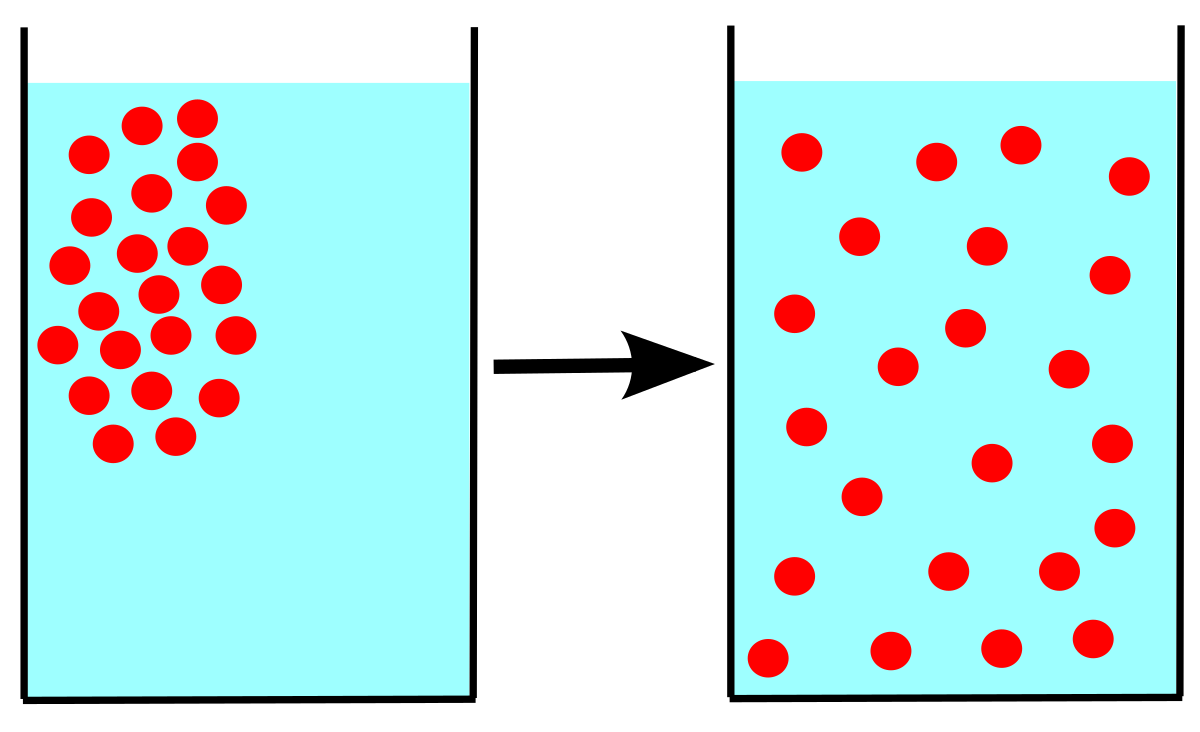
\includegraphics[scale=0.15]{./images/diffusion.png}
%		\caption{Disffusion.}
%		\label{fig:diffusion}
%	\end{figure}
% \vskip0pt plus 1filll
% \href{https://arxiv.org/abs/1503.03585}{\tiny \blue{ICML 2015 Deep Unsupervised Learning using Nonequilibrium Thermodynamics}}

	The overall idea is to construct a Markov chain of progressively less noisy samples. Each transition denoises a noisy sample. Diffusion models consist of two Markov chains:
	\begin{enumerate}
		\item Forward: A Markov chain of diffusion steps to \textbf{slowly add random noise} to data. 
			$$\rvx_0\to \rvx_1\cdots\to \rvx_T$$
		\item Backward (Reverse): Learn to \textbf{reverse the diffusion process} to construct desired data samples from the noise. 
			$$\rvx_T\to \rvx_{T-1}\cdots\to \rvx_0$$
	\end{enumerate}
	\begin{figure}[t]
		\centering
		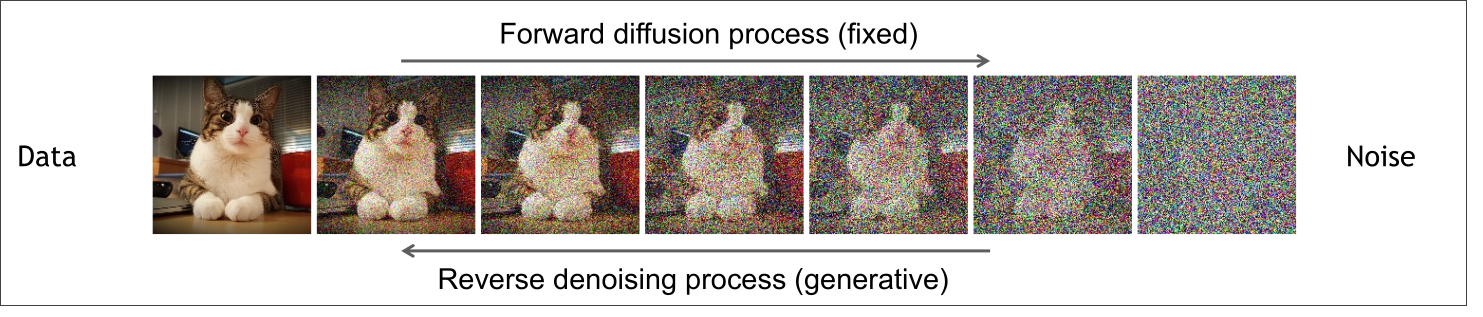
\includegraphics[scale=0.28]{./images/diffusion/diffusion_model.png}
	\end{figure}
	% \href{https://cvpr2022-tutorial-diffusion-models.github.io/}{\tiny \blue{CVRP 2022 Tutorial: Denoising Diffusion-based Generative Modeling: Foundations and Applications}}

\textbf{Some properties of diffusion models}:
	\begin{enumerate}
		%$$q(\rvx_t|\rvx_{t-1}) = \mathcal{T}(\rvx_t|\rvx_{t-1})$$
		\item Diffusion model has a pre-defined sampling equation.
			\begin{itemize}
				\item The equation relies on a random noise.
				\item Noise is all we need $\to$ Predict noise at a time step $t$.
			\end{itemize}
		\item Fit a model via forward and backward processes.
		\item \textbf{Iterative transform} of one distribution into another via \textbf{Makov Chain}.
			\begin{itemize}
				\item $\mathcal{D}_{data}\to \mathcal{N}$.
				\item $\mathcal{N}\to \mathcal{D}_{data}$.
				\item Diffusion model$\approx$Generative Markov Chain.
			\end{itemize}
		\item Learn a transition model:
			$$p_\theta(\mathbf{x}_{t-1}|x_t) = \mathcal{N}(\mathbf{x}_{t-1}|\boldsymbol{\mu}_{\theta}(\mathbf{x}_{t}, t), \boldsymbol{\Sigma}_\theta(\mathbf{x}_t,t)).$$
		\item Base case: $p(\mathbf{x}_T) = \mathcal{N}(0,I)$ 
		\item Marginal distribution over $\mathbf{x}_0$:
			$$p_\theta(\mathbf{x}_0) = \int p_\theta(\rvx_0,\dots,\mathbf{x}_T)d\rvx_1,\dots,\rvx_T$$
		\item We want to learn the parameters so that
			$$p(\rvx_0)\approx p_\theta(\rvx_0)$$

	\end{enumerate}

\section{Forward Diffusion}

	\begin{itemize}
		\item We want to model a forward trajectory (by the Markov property): 
			$$q(\mathbf{x}_{0:T}) = q(\rvx_0)\prod^T_{t=1} \underbrace{q(\mathbf{x}_t \vert \mathbf{x}_{t-1})}_{\text{Transition kernel}} $$
		\item Slow transform with a large $T$: $\rvx_0\to \rvx_1\cdots\to \rvx_T$
			\begin{itemize}
				\item Imagine someone said he is from Germany.
				\item We can't exactly track his journey without more information.
				\item We need to add more steps!
			\end{itemize}
		\item How to model $q(\mathbf{x}_t \vert \mathbf{x}_{t-1})$?
%		\item By the Markov property, $q$ is given by
%			$$q(\mathbf{x}_{1:T} \vert \mathbf{x}_0) &=  \prod^T_{t=1} q(\mathbf{x}_t \vert \mathbf{x}_{t-1})$$
		%\item $q(\mathbf{x}_t \vert \mathbf{x}_{t-1}) = $
	\end{itemize}

Forward Diffusion: $q(\rvx_t \vert \rvx_{t-1})$
	In a continuous case (\eg image), each transition can be parameterized as follows:
\begin{align}
	q(\rvx_t \vert \rvx_{t-1}) &= \mathcal{N}(\mathbf{x}_t; \sqrt{1 - \beta_t} \rvx_{t-1}, \beta_t\mathbf{I})
	\label{eq:forward_diffusion}
\end{align}
\begin{itemize}
		\item $\beta_t\in (0,1)$ is a variance at time $t$.
		\item $\sqrt{1 - \beta_t}$ downscales $\rvx_{t-1}$ to be 0, $\beta_1<\cdots<\beta_t$. Thus, $\rvx_t$ will become more noisier. $\rvx_t$ can be sampled as:
			$$\mathbf{x}_t= \sqrt{1 - \beta_t} \mathbf{x}_{t-1}+ \sqrt{\beta_t} \odot \epsilon$$
			\begin{enumerate}
				\item Sample $\rvx_{t}\sim q(\rvx_t)$ and scale it by $\sqrt{1 - \beta_t}$
				\item Adds noise $\epsilon\sim \mathcal{N}(0,I)$ with variance $\beta_t$.
			\end{enumerate}
		\item The above process is autoregressive (\ie ancestral sampling), but we can sample $\mathbf{x}_t$ directly from $q(\mathbf{x}_t|\rvx_0)$ in an analytic form:
\begin{align}
	\rvx_t &= \sqrt{1 - \beta_t} \mathbf{x}_{t-1}+ \sqrt{\beta_t} \odot \epsilon_{t-1}\\
						   &= \sqrt{\alpha_t} \mathbf{x}_{t-1}+ \sqrt{1-\alpha_t} \odot \epsilon_{t-1}\\
						   &= \sqrt{\alpha_t} \bigg(\sqrt{\alpha_{t-1}} \mathbf{x}_{t-2}+ \sqrt{1-\alpha_{t-1}} \odot \epsilon_{t-2}\bigg) + \sqrt{1-\alpha_t} \odot \epsilon_{t-1}\\
						   &= \sqrt{\alpha_t\alpha_{t-1}} \mathbf{x}_{t-2} + \sqrt{\alpha_t-\alpha_t\alpha_{t-1}} \odot \epsilon_{t-2} + \sqrt{1-\alpha_t} \odot \epsilon_{t-1}\\
						   &= \sqrt{\alpha_t\alpha_{t-1}} \mathbf{x}_{t-2} + \sqrt{\alpha_t-\alpha_t\alpha_{t-1}+1-\alpha_t} \odot \epsilon_{t-2} \\
						   &= \sqrt{\alpha_t\alpha_{t-1}} \mathbf{x}_{t-2} + \sqrt{1-\alpha_t\alpha_{t-1}} \odot \epsilon_{t-2} \\
						   &= \dots\\
						   &= \sqrt{\prod_{t}\alpha_t} \mathbf{x}_{0} + \sqrt{1-\prod_t \alpha_t} \odot \epsilon_{t_0} \\
						   &= \sqrt{\bar{\alpha}_t} \mathbf{x}_{0}+ \sqrt{1-\bar{\alpha}_t} \odot \epsilon\\
	&\sim \mathcal{N}(\mathbf{x}_t; \sqrt{\bar{\alpha}_t} \rvx_{0}, (1-\bar{\alpha}_t)\mathbf{I}),
	% &= q(\mathbf{x}_t|\rvx_{0}), 
	\label{eq:diffusion_forward_sampling}
\end{align}
			where $\alpha_t = 1-\beta_t$ and $\bar{\alpha}_t = \prod_{s=1}^t \alpha_s$. Thus, $\mathbf{x}_t= \sqrt{\bar{\alpha}_t} \mathbf{x}_{0}+ \sqrt{1-\bar{\alpha}_t} \odot \epsilon$. Note that the fifth step is done by using the property of sum of two Gaussian distributions (\eg $\mathcal{N}(0, \sigma_1^2I)+\mathcal{N}(0, \sigma_2^2I) = \mathcal{N}(0, (\sigma_1^2+\sigma_2^2)I)$ ). 
\end{itemize}

We can get some intuitions:
\begin{itemize}
	\item The original input $\rvx_0$ \textbf{gradually loses all info} during the forward diffusion process.
	\item This Markov chain has a \textbf{stationary distribution}: As $t\to \infty$, $q(\rvx_t) \approx \mathcal{N}(0,I)$.
		\begin{itemize}
			\item In practice, $T$ is a very high number \eg 1,000.
			\item Minimize info loss for each step.
			\item Allow a smooth training.
		\end{itemize}
\end{itemize}

%\begin{frame}{Forward Diffusion: $q(\rvx_t)$}
%	\begin{align*}
%		\underbrace{q(x_t)}_{\text{diffused data dist.}} = \int \underbrace{q(x_t,x_0)}_{\text{Joint dist.}} dx_0 = \int \underbrace{q(x_0)}_{\text{Input dist.}}\underbrace{q(x_t|x_0)}_{\text{Diffusion kernel}} dx_0 .
%	\end{align*}
%	\begin{itemize}
%		\item We can sample $\rvx_t\sim q(\rvx_t)$ by first sampling $\rvx_0\sim q(\rvx_0)$
%		\item Sample $\rvx_t$ at any arbitrary noise level without iterative computations.
%		\item $\rvx_t = \sqrt{\bar{\alpha}_t}\rvx_0+\sqrt{(1-\bar{\alpha}_t)}\epsilon$ : reparameterization
%		\item $\alpha_t:=1-\beta_t$
%		\item $\bar{\alpha}_t:=\prod_{i=1}^t\alpha_i$
%		\item \red{Why sampling $\rvx_t$?}
%	\end{itemize}
%\end{frame}

%\begin{frame}{Forward Diffusion}
%	\begin{itemize}
%		\item Diffusion kernel: 
%			$$q(x_t|x_0) = \mathcal{N}(\sqrt{\bar{\alpha}_t}x_0, (1-\bar{\alpha}_t)I )$$
%		\item[] $\approx$ Gaussian convolution.
%		\item We can sample $x_t$ by adding scaled noise to $x_0$.
%		\item $\beta_t$ value is scheduled to be $\bar{\alpha}_T\to 0$ and $q(x_t|x_0)\approx \mathcal{N}(x_T;0,I)$
%	\end{itemize}
%\end{frame}



\section{Backward Process}

Generative Learning by Denoising:
	\begin{itemize}
		\item Now we know how to model the forward process (diffusion process).
		\item However, a noisy image is not what we want.
		\item We want to generate a new image with high quality.
	\end{itemize}

	How to generate data? If we can reverse the forward process, then we can draw a true sample. We call it \textbf{Backward process}!
	\begin{itemize}
		\item Start from $q(\rvx_T)\approx \mathcal{N}(0,I)$.
		\item Sample $\rvx_T\sim \mathcal{N}(\rvx_T|0,I)$
			\begin{itemize}
				\item Sample a noise vector from a prior distribution.
			\end{itemize}
		\item Iteratively sample $\rvx_{t-1}\sim q(\rvx_{t-1}|\rvx_t).$ 
			\begin{itemize}
				\item $q(\rvx_{t-1}|\rvx_t)$: \textbf{true denoising distribution} (we don't know).
			\end{itemize}
		\item In general, $q(\rvx_{t-1}|\rvx_t)$ is intractable.
		%\item In general, $q(x_{t-1}|x_t)\propto q(x_{t-1})q(x_t|x_{t-1})$ is intractable.
		\item We can \textbf{approximate} $q(\rvx_{t-1}|\rvx_t)$ as \textbf{Normal distribution} if $\beta_t$ is small in each forward diffusion step.
			\begin{itemize}
				\item \eg $\rvx_3$ to $\rvx_2$
			\end{itemize}
	\end{itemize}
	\begin{figure}[h]
		\centering
		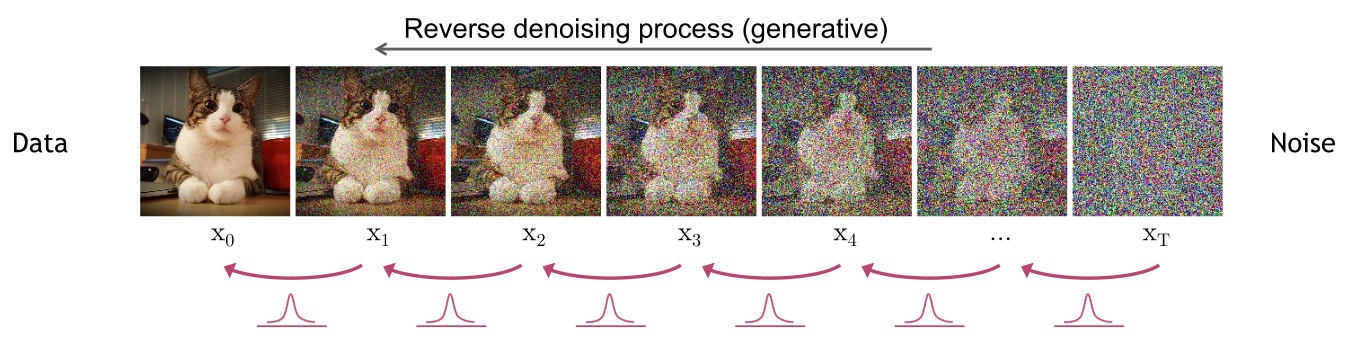
\includegraphics[scale=0.30]{./images/diffusion/reverse.png}
	\end{figure}
	\href{https://cvpr2022-tutorial-diffusion-models.github.io/}{\tiny \blue{CVPR 2022 Tutorial: Denoising Diffusion-based Generative Modeling: Foundations and Applications}}

Backward Process
	\begin{itemize}
%		\item Reverse the forward process
%			\begin{itemize}
%					\item Sample from the \textbf{exact reverse distribution} $q(\rvx_{t-1}|\rvx_t)$ (true denoising dist.), 
%					\item Recreate the true sample from a Gaussian noise input $\rvx_T\sim \mathcal{N}(0,I)$.
%				\end{itemize}
		%\item The reversal of the disffusion process has the identical form as the forward process.
		%\item The longer the trajectory the smaller the diffusion rate $\beta$ can be made.
		\item Approximate $q(\rvx_{t-1}|\rvx_t)$ using a neural network, $p_\theta(\mathbf{x}_{t-1} \vert \mathbf{x}_t)$.
		\item Backward process: $p_\theta(\mathbf{x}_{0:T}) = p(\mathbf{x}_T) \prod^T_{t=1} p_\theta(\mathbf{x}_{t-1} \vert \mathbf{x}_t)$.
			\begin{itemize}
				\item $p(\rvx_T) = \mathcal{N}(\rvx_T;0,I)$.
				\item $p_\theta(\mathbf{x}_{t-1} \vert \mathbf{x}_t) = \mathcal{N}(\mathbf{x}_{t-1}; \boldsymbol{\mu}_\theta(\mathbf{x}_t, t), \boldsymbol{\Sigma}_\theta(\mathbf{x}_t, t))$.  

				\item We can model the denoising distribution as Normal distribution like above (\cf \Cref{eq:diffusion_kl_true_denoising}).
				\item Note that the reverse conditional probability $q(\rvx_{t-1}|\rvx_t)$ is tractable when it is conditioned on $\rvx_0$ as shown in \Cref{eq:diffusion_kl_true_denoising}. This allows us to train a neural network to model this denoising distribution. 
			\end{itemize}
			% \begin{itemize}
			% 	\item Network outputs mean and variance ($\boldsymbol{\mu}_{\theta}$ and $\boldsymbol{\Sigma}_{\theta}$). 
			% 	\item We are not going to make a model to predict them directly.
			% 	\item \textbf{Train a noise prediction network.}
			% \end{itemize}
		\item Key to the success of this sampling process is training the reverse Markov chain to match the actual time reversal of the forward Markov chain. 
		\item After optimizing the backward process, the sampling procedure is that just sample Gaussian noise from $p(\rvx_T)$ and then iteratively running the denoising transitions (backward process) for T steps to generate a novel $\rvx_0$.
	\end{itemize}


\section{Distribution Modeling}
	What we want to learn (or model) is $p_\theta(\rvx_0)\approx p(\rvx_0)$ (approximate data distribution).
	\begin{itemize}
%		\item $p_\theta(\rvx_0)$: a distribution of output (denoised) image.
%			\begin{itemize}
%				\item This is our target.
%			\end{itemize}
		\item $p_\theta(\rvx_0) = \int p_\theta(\rvx_{0:T})d\rvx_{1:T}$
		\item It is intractable to compute all trajectories.
			$$\argmax_\theta\mathbb{E}_{\rvx_0\sim p}[\log p_\theta(\rvx_0)] = \mathbb{E}_{\rvx_0\sim p}\bigg[\log\int p_\theta(\rvx_{0:T})d\rvx_{1:T}\bigg].$$
		\item Thus, we will use variational lower bound with KL-Div:
	\end{itemize}
\begin{align}
\log p_\theta(\rvx_0) 
	&=  \log\int p(\rvx_{0:T})d\rvx_{1:T}\\
	&= \log\int p(\rvx_{0:T})\frac{q(\rvx_{1:T}|\rvx_0)}{q(\rvx_{1:T}|\rvx_0)}d\rvx_{1:T}\\
	&= \log\int q(\rvx_{1:T}|\rvx_0)\frac{p(\rvx_{0:T})}{q(\rvx_{1:T}|\rvx_0)}d\rvx_{1:T}\\
	&\geq \int q(\rvx_{1:T}|\rvx_0)\log\frac{p(\rvx_{0:T})}{q(\rvx_{1:T}|\rvx_0)}d\rvx_{1:T}\\
	&= \mathbb{E}_{q(\rvx_{1:T}|\rvx_0)}\bigg[\log\frac{p(\rvx_{0:T})}{q(\rvx_{1:T}|\rvx_0)}\bigg] \quad \to \textrm{ELBO}\\
	&= \mathbb{E}_{q(\rvx_{1:T}|\rvx_0)}\bigg[\log p(\rvx_T)\prod_{t=1}^T\frac{p(\rvx_{t-1}|\rvx_t)}{q(\rvx_{t}|\rvx_{t-1})}\bigg]\\
	&= \mathbb{E}_{q(\rvx_{1:T}|\rvx_0)}\bigg[\log \frac{p(\rvx_T)p(\rvx_0|\rvx_{1})\prod_{t=1}^{T-1} p(\rvx_{t}|\rvx_{t+1})}{q(\rvx_T|\rvx_{T-1})\prod_{t=1}^{T-1}  q(\rvx_{t}|\rvx_{t-1})}\bigg]\\
	&= \mathbb{E}_{q(\rvx_{1:T}|\rvx_0)}\bigg[\log \frac{p(\rvx_T)p(\rvx_0|\rvx_{1})}{q(\rvx_T|\rvx_{T-1})}\bigg] + \mathbb{E}_{q(\rvx_{1:T}|\rvx_0)}\bigg[\log \prod_{t=1}^{T-1}\frac{ p(\rvx_{t}|\rvx_{t+1})}{q(\rvx_{t}|\rvx_{t-1})}\bigg]\\
	&= \mathbb{E}_{q(\rvx_{1:T}|\rvx_0)}[\log p(\rvx_0|\rvx_{1})]+\mathbb{E}_{q(\rvx_{1:T}|\rvx_0)}\bigg[\log \frac{p(\rvx_T)}{q(\rvx_T|\rvx_{T-1})}\bigg]\\ 
	&\quad + \mathbb{E}_{q(\rvx_{1:T}|\rvx_0)}\bigg[\sum_{t=1}^{T-1}\log \frac{ p(\rvx_{t}|\rvx_{t+1})}{q(\rvx_{t}|\rvx_{t-1})}\bigg]\\
	&= \dots + \blue{\mathbb{E}_{q(\rvx_{1:T}|\rvx_0)}\bigg[\log \frac{p(\rvx_T)}{q(\rvx_T|\rvx_{T-1})}\bigg]} + \sum_{t=1}^{T-1}\mathbb{E}_{q(\rvx_{1:T}|\rvx_0)}\bigg[\log \frac{ p(\rvx_{t}|\rvx_{t+1})}{q(\rvx_{t}|\rvx_{t-1})}\bigg]\\
	% % &= \log\int q(\rvx_{1:T}|\rvx_0)p(\rvx_T)\prod_{t=1}^T\frac{p(\rvx_{t-1}|\rvx_t)}{q(\rvx_{t}|\rvx_{t-1})}d\rvx_{1:T}
		&= \dots + \int_{x_1}\dots\int_{x_T}q(\rvx_{1},\dots,\rvx_{T})\bigg[\log \frac{p(\rvx_T)}{q(\rvx_T|\rvx_{T-1})}\bigg]dx_1\dots dx_T + \dots\\
		&= \dots + \int_{x_T}\int_{x_{T-1}}\bigg[\log \frac{p(\rvx_T)}{q(\rvx_T|\rvx_{T-1})}\bigg]\dots\int_{x_1} q(\rvx_{1},\dots,\rvx_{T})dx_1\dots dx_T + \dots\\
		&= \dots + \int_{x_T}\int_{x_{T-1}}\bigg[\log \frac{p(\rvx_T)}{q(\rvx_T|\rvx_{T-1})}\bigg] q(\rvx_{t},\rvx_{t-1})dx_{T-1} dx_T + \dots\\
		&= \dots + \mathbb{E}_{q(\rvx_{t}, \rvx_{t-1}|\rvx_0)}\bigg[\log \frac{p(\rvx_T)}{q(\rvx_T|\rvx_{T-1})}\bigg] + \sum_{t=1}^{T-1}\mathbb{E}_{q(\rvx_{t-1},\rvx_t,\rvx_{t+1}|\rvx_0)}\bigg[\log \frac{ p(\rvx_{t}|\rvx_{t+1})}{q(\rvx_{t}|\rvx_{t-1})}\bigg]\\
		&= \mathbb{E}_{q(\rvx_{1}|\rvx_0)}[\log p(\rvx_0|\rvx_{1})] + \mathbb{E}_{q(\rvx_{t}, \rvx_{t-1}|\rvx_0)}\bigg[\log \frac{p(\rvx_T)}{q(\rvx_T|\rvx_{T-1})}\bigg]\\ 
		&\quad+ \sum_{t=1}^{T-1}\mathbb{E}_{q(\rvx_{t-1},\rvx_t,\rvx_{t+1}|\rvx_0)}\bigg[\log \frac{ p(\rvx_{t}|\rvx_{t+1})}{q(\rvx_{t}|\rvx_{t-1})}\bigg]\\
		&= \mathbb{E}_{q(\rvx_{1}|\rvx_0)}[\log p(\rvx_0|\rvx_{1})] - \mathbb{E}_{q(\rvx_{t-1}|\rvx_0)}[D_{KL}(q(\rvx_T|\rvx_{T-1})\| p(\rvx_T))]\\
		&\,- \sum_{t=1}^{T-1}\mathbb{E}_{q(\rvx_{t-1},\rvx_{t+1}|\rvx_0)}D_{KL}[q(\rvx_{t}|\rvx_{t-1})\|p(\rvx_{t}|\rvx_{t+1})]\\
		& \because q(\rvx_{t}, \rvx_{t-1}|\rvx_0) = \frac{q(\rvx_{t}, \rvx_{t-1},\rvx_0)}{q(\rvx_0)} = \frac{q(\rvx_{t}|\rvx_{t-1}, \rvx_0)q(\rvx_{t-1}, \rvx_0)}{q(\rvx_0)} = q(\rvx_{t}|\rvx_{t-1})q(\rvx_{t-1}|\rvx_0)
	% % &= \log\int q(\rvx_{1:T}|\rvx_0)p(\rvx_T)\prod_{t=1}^T\frac{p(\rvx_{t-1}|\rvx_t)}{q(\rvx_{t}|\rvx_{t-1})}d\rvx_{1:T}
	\label{eq:diffusion_mle}
\end{align}
\begin{itemize}
	\item The sixth step is done by Markov property.
	\item The first term is a \textit{reconstruction term}. 
	\item The second term is a \textit{prior matching term}. This term requires no optimization, as it has no trainable parameters; furthermore, as we have assumed a large enough $T$ such that the final distribution is Gaussian, this term effectively becomes zero.
	\item The last term is a \textit{consistency term}. It endeavors to make the distribution at xt consistent, from both forward and backward processes. That is, a denoising step from a noisier image should match the corresponding noising step from a cleaner image, for every intermediate timestep.  This term is minimized when we train $p_\theta(\rvx_t|\rvx_{t+1})$ to match the Gaussian distribution $q(\rvx_t|\rvx_{t-1})$, which is defined in \Cref{eq:forward_diffusion}. % \item For a small $\beta$, the forward and the backward processes can be identical.
	\item Under this derivation, all terms of the ELBO are computed as expectations, and can therefore be approximated using Monte Carlo estimates. 
	\item However, actually optimizing the ELBO using the terms we just derived might be suboptimal, because the consistency term is computed as an expectation over two random variables $\{x_{t-1}, x_{t+1}\}$ for every time step, the variance of its Monte Carlo estimate could potentially be higher than a term that is estimated using only one random variable per time step. As it is computed by summing up $T-1$ consistency terms, the final estimated value of the ELBO may have high variance for large $T$ values.
\end{itemize}

Let us instead try to derive a form for our ELBO where each term is computed as an expectation over \textbf{only one random variable at a time}. The key insight is that we can rewrite encoder transitions as $q(x_t|x_{t-1}) = q(x_t|x_{t-1}, x_0)$, where the extra conditioning term is superfluous due to the Markov property. Then, according to Bayes rule, we can rewrite each transition as:
\begin{align*}
	q(\rvx_t|\rvx_{t-1}, \rvx_0)= \frac{q(\rvx_{t-1}|\rvx_t, \rvx_0)q(\rvx_t| \rvx_0)}{q(\rvx_{t-1}| \rvx_0)} 
\end{align*}
Armed with this equation, we can factorize the ELBO again as follows:
\begin{align}
		L &= \mathbb{E}_{q(\rvx_{1:T}|\rvx_0)}\bigg[\log\frac{p(\rvx_{0:T})}{q(\rvx_{1:T}|\rvx_0)}\bigg] \quad \to \textrm{ELBO}\\		
		&= \mathbb{E}_{q(\rvx_{1:T}|\rvx_0)}\bigg[\log p(\rvx_T)\prod_{t=1}^T\frac{p(\rvx_{t-1}|\rvx_t)}{q(\rvx_{t}|\rvx_{t-1})}\bigg]\\
		&= \mathbb{E}_{q(\rvx_{1:T}|\rvx_0)}\bigg[\log \frac{p(\rvx_T)p(\rvx_0|\rvx_{1})\prod_{t=2}^{T} p(\rvx_{t-1}|\rvx_{t})}{q(\rvx_1|\rvx_{0})\prod_{t=2}^{T}  q(\rvx_{t}|\rvx_{t-1})}\bigg]\\
		&= \mathbb{E}_{q(\rvx_{1:T}|\rvx_0)}\bigg[\log \frac{p(\rvx_T)p(\rvx_0|\rvx_{1})\prod_{t=2}^{T} p(\rvx_{t-1}|\rvx_{t})}{q(\rvx_1|\rvx_{0})\prod_{t=2}^{T}  q(\rvx_{t}|\rvx_{t-1}, \blue{\rvx_0})}\bigg] \quad \textrm{ by Markov Property}\\
		&= \mathbb{E}_{q(\rvx_{1:T}|\rvx_0)}\bigg[\log \frac{p(\rvx_T)p(\rvx_0|\rvx_{1})}{q(\rvx_1|\rvx_{0})}+\log \prod_{t=2}^{T}\frac{ p(\rvx_{t-1}|\rvx_{t})}{q(\rvx_{t}|\rvx_{t-1}, \rvx_0)}\bigg]\\
		&= \mathbb{E}_{q(\rvx_{1:T}|\rvx_0)}\bigg[\log \frac{p(\rvx_T)p(\rvx_0|\rvx_{1})}{q(\rvx_1|\rvx_{0})}+\log \prod_{t=2}^{T}\frac{ p(\rvx_{t-1}|\rvx_{t})}{\frac{q(\rvx_{t-1}|\rvx_t, \rvx_0)q(\rvx_t| \rvx_0)}{q(\rvx_{t-1}| \rvx_0)}}\bigg]\\
		&= \mathbb{E}_{q(\rvx_{1:T}|\rvx_0)}\bigg[\log \frac{p(\rvx_T)p(\rvx_0|\rvx_{1})}{q(\rvx_1|\rvx_{0})}+\log \frac{q(\rvx_1|\rvx_0)}{q(\rvx_T|\rvx_0)}+\log \prod_{t=2}^{T}\frac{ p(\rvx_{t-1}|\rvx_{t})}{q(\rvx_{t-1}|\rvx_t, \rvx_0)}\bigg]\\
		&= \mathbb{E}_{q(\rvx_{1:T}|\rvx_0)}\bigg[\log \frac{p(\rvx_T)p(\rvx_0|\rvx_{1})}{q(\rvx_T|\rvx_{0})}+\log \prod_{t=2}^{T}\frac{ p(\rvx_{t-1}|\rvx_{t})}{q(\rvx_{t-1}|\rvx_t, \rvx_0)}\bigg]\\
		&= \mathbb{E}_{q(\rvx_{1}|\rvx_0)}[\log p(\rvx_0|\rvx_{1})]+\mathbb{E}_{q(\rvx_{T}|\rvx_0)}\bigg[\log \frac{p(\rvx_T)}{q(\rvx_T|\rvx_{0})}\bigg]+\ \sum_{t=2}^{T}\mathbb{E}_{q(\rvx_{t},\rvx_{t-1}|\rvx_0)}\bigg[\log\frac{ p(\rvx_{t-1}|\rvx_{t})}{q(\rvx_{t-1}|\rvx_t, \rvx_0)}\bigg]\\
		&= \mathbb{E}_{q(\rvx_{1}|\rvx_0)}[\log p(\rvx_0|\rvx_{1})]-D_{KL}_(q(\rvx_{T}|\rvx_0)||p(\rvx_T))-\sum_{t=2}^{T}\mathbb{E}_{q(\rvx_{t}|\rvx_0)}[D_{KL}(q(\rvx_{t-1}|\rvx_t, \rvx_0)\|p(\rvx_{t-1}|\rvx_{t}))]
		% &= \mathbb{E}_{q(\rvx_{1:T}|\rvx_0)}\bigg[\log \frac{p(\rvx_T)p(\rvx_0|\rvx_{1})}{q(\rvx_T|\rvx_{T-1})}\bigg] + \mathbb{E}_{q(\rvx_{1:T}|\rvx_0)}\bigg[\log \prod_{t=1}^{T-1}\frac{ p(\rvx_{t}|\rvx_{t+1})}{q(\rvx_{t}|\rvx_{t-1})}\bigg]\\
% 		&= \mathbb{E}_{q}\Bigg[-\log p_\theta(x_T)-\log\frac{\prod_{t=1}^Tp_\theta(x_{t-1}|x_t)}{\prod_{t=1}^Tq(x_{t}|x_{t-1})}\Bigg]\\
% 		&= \mathbb{E}_{q}\Bigg[-\log p_\theta(x_T)-\sum_{t\geq 1}\log\frac{p_\theta(x_{t-1}|x_t)}{q(x_{t}|x_{t-1})}\Bigg]\\
% 		&= \mathbb{E}_{q}\Bigg[-\log p_\theta(x_T)-\sum_{t=2}^T\log\frac{p_\theta(x_{t-1}|x_t)}{q(x_{t}|x_{t-1})}-\log \frac{p_\theta(x_{0}|x_1)}{q(x_{1}|x_{0})}\Bigg]\\
% 		&= \mathbb{E}_{q}\Bigg[-\log p_\theta(x_T)-\sum_{t=2}^T\log\frac{p_\theta(x_{t-1}|x_t)}{q(x_{t-1}|x_{t},x_0)}\cdot \red{ \frac{q(x_{t-1}|x_0)}{q(x_{t}|x_0)}}\\
% 		&\quad -\log \frac{p_\theta(x_{0}|x_1)}{q(x_{1}|x_{0})}\Bigg]\\
	\label{eq:diffusion_objective}
\end{align}
Let's closely look at the last three terms:
\begin{itemize}
	\item $\mathbb{E}_{q(\rvx_{1}|\rvx_0)}[\log p(\rvx_0|\rvx_{1})]$: reconstruction term. 
	\item $D_{KL} (q(\rvx_{T}|\rvx_0)||p(\rvx_T))$: Prior matching term.
		\begin{itemize}
			\item No trainable parameters 
		\end{itemize}
	\item $\sum_{t=2}^{T}\mathbb{E}_{q(\rvx_{t}|\rvx_0)}[D_{KL}(q(\rvx_{t-1}|\rvx_t, \rvx_0)\|p(\rvx_{t-1}|\rvx_{t}))]$: Denoising matching term.
		\begin{itemize}
			\item $p_\theta(\rvx_{t−1}|\rvx_t)$ as an approximation to tractable, ground-truth denoising transition step $q(\rvx_{t−1}|\rvx_t, \rvx_0)$. The $q(\rvx_{t−1}|\rvx_t, \rvx_0)$ transition step can act as a ground-truth signal, since it defines how to denoise a noisy image with access to what the final, completely denoised image $\rvx_0$ should be. This term is therefore minimized when the two denoising steps match as closely as possible, as measured by their KL Divergence.
		\end{itemize}
\end{itemize}
In the last term, $q(\rvx_{t-1}|\rvx_t, \rvx_0)$ can be further factorized as follows:
\begin{align*}
	q(\rvx_{t-1}|\rvx_t, \rvx_0) = \frac{q(\rvx_{t}|\rvx_{t-1}, \rvx_0)q(\rvx_{t-1}|\rvx_0)}{q(\rvx_{t}|\rvx_0)}=\frac{q(\rvx_{t}|\rvx_{t-1})q(\rvx_{t-1}|\rvx_0)}{q(\rvx_{t}|\rvx_0)}.
\end{align*}
Then, $q(\rvx_{t}|\rvx_{t-1}, \rvx_0) = q(\rvx_{t}|\rvx_{t-1})$ by Markov property. Now, let's compute the KL-divergence in the denoising matching term. 

\begin{align}
	q(\rvx_{t-1}|\rvx_t, \rvx_0) &=\frac{q(\rvx_{t}|\rvx_{t-1})q(\rvx_{t-1}|\rvx_0)}{q(\rvx_{t}|\rvx_0)}\\
								 &= \frac{\mathcal{N}(\mathbf{x}_t; \sqrt{\bar{\alpha}_t} \rvx_{t-1}, (1-\bar{\alpha}_t)\mathbf{I})\mathcal{N}(\mathbf{x}_{t-1}; \sqrt{\bar{\alpha}_{t-1}} \rvx_{0}, (1-\bar{\alpha}_{t-1})\mathbf{I})}{\mathcal{N}(\mathbf{x}_t; \sqrt{\bar{\alpha}_t} \rvx_{0}, (1-\bar{\alpha}_t)\mathbf{I})}\\
								 & \vdots\\
								 &\propto \mathcal{N}\bigg(\rvx_{t-1};\underbrace{\frac{\sqrt{{\alpha}_{t}}(1-\bar{\alpha}_{t-1})\rvx_t+\sqrt{\bar{\alpha}_{t-1}}(1-{\alpha}_{t})\rvx_0}{1-\bar{\alpha}_{t}}}_{\mu_q(\rvx_t,\rvx_0)}, \underbrace{\frac{(1-{\alpha}_{t})(1-\bar{\alpha}_{t-1})}{1-\bar{\alpha}_{t}}\mathbf{I}}_{\Sigma_{q}(t)}\bigg)
	\label{eq:diffusion_kl_true_denoising}
\end{align}

We have therefore shown that at each step, $\rvx_{t-1} \sim q(\rvx_{t-1}|\rvx_t, \rvx_0)$ is normally distributed, with mean $\mu_q(\rvx_t,\rvx_0)$ that is a function of $\rvx_t$ and $\rvx_0$, and variance $\Sigma_q(t)$ as a function of $\alpha$ coefficients. 

% These $\alpha$ coefficients are known and fixed at each time step; they are either set permanently when modeled as hyperparameters, or treated as the current inference output of a network that seeks to model them. We can rewrite the variance equation as $\Sigma_q(t) = \sigma^2_q(t)I$, where:
% $$\sigma^2_q(t) = \frac{(1-{\alpha}_{t})(1-\bar{\alpha}_{t-1})}{1-\bar{\alpha}_{t}}.$$
% In order to match approximate denoising transition step $p_\theta(\rvx_{t-1}|\rvx_{t})$ to ground-truth denoising transition step $q(\rvx_{t-1}|\rvx_t, \rvx_0)$ as closely as possible, we can also model it as a Gaussian. Furthermore, as all $\alpha$ terms are known to be frozen at each timestep, we can immediately construct the variance of the approximate denoising transition step to also be $\Sigma_q(t) = \sigma^2_q(t)I$.

% The following equation is the KL divergence between two normal distributions $P$ and $Q$:
% $$D_{KL}(P\|Q) = \frac{1}{2}\left[\log\frac{|\Sigma_2|}{|\Sigma_1|} - n + \text{tr} \{ \Sigma_2^{-1}\Sigma_1 \} + (\mu_2 - \mu_1)^T \Sigma_2^{-1}(\mu_2 - \mu_1)\right]$$
% We can optimize the KL divergence between two normal distributions to minimize the difference between the two means: 
% \begin{align}
% 	\mathcal{L} &= \min_\theta D_{KL}(q(\rvx_{t-1}|\rvx_t, \rvx_0)\|p_\theta(\rvx_{t-1}|\rvx_{t}))\\
% 				& \vdots\\
% 				&= \min_\theta \frac{1}{2\sigma^2_q(t)}\big[\|\boldsymbol{\mu}_\theta- \boldsymbol{\mu}_q\|^2_2\big],
% 	\label{eq:diffusion_kl_mean}
% \end{align}
% where $\boldsymbol{\mu}_q$ is a shorthand for $\boldsymbol{\mu}_q(\rvx_t,\rvx_0)$.

We can use the \Cref{eq:diffusion_kl_true_denoising} to compute the optimal $\theta$ by solving $\min_\theta D_{KL}(q(\rvx_{t-1}|\rvx_t, \rvx_0)\|p_\theta(\rvx_{t-1}|\rvx_{t}))$, but we can simplify the optimization problem by using \Cref{eq:diffusion_forward_sampling}:
\begin{align*}
	\rvx_t &= \sqrt{\bar{\alpha}_t} \mathbf{x}_{0}+ \sqrt{1-\bar{\alpha}_t} \odot \epsilon\\
	\mathbf{x}_{0} &= \frac{\rvx_t - \sqrt{1-\bar{\alpha}_t}\odot \epsilon}{\sqrt{\bar{\alpha}_t} } 
\end{align*}
By plugging the above equation into $\boldsymbol{\mu}_q(\rvx_t,\rvx_0)$, we can exclude $\rvx_0$ term as follows:
\begin{align}
	\boldsymbol{\mu}_q(\rvx_t,\rvx_0) &= \frac{\sqrt{{\alpha}_{t}}(1-\bar{\alpha}_{t-1})\rvx_t+\sqrt{\bar{\alpha}_{t-1}}(1-{\alpha}_{t})\rvx_0}{1-\bar{\alpha}_{t}}\\
									  &= \frac{\sqrt{{\alpha}_{t}}(1-\bar{\alpha}_{t-1})\rvx_t+\sqrt{\bar{\alpha}_{t-1}}(1-{\alpha}_{t})\frac{\rvx_t - \sqrt{1-\bar{\alpha}_t}\odot \epsilon}{\sqrt{\bar{\alpha}_t} }}{1-\bar{\alpha}_{t}}\\
									  &\vdots\\
									  &= \frac{1}{\sqrt{\alpha_t}}\rvx_t - \frac{1-\alpha_t}{\sqrt{1-\bar{\alpha_t}}\sqrt{\alpha_t}}\boldsymbol{\epsilon}_0
	\label{eq:diffusion_mean_simple}
\end{align}
Thus, we can force $\boldsymbol{\mu}_\theta(\mathbf{x}_t, t)$, which has no dependency on $\rvx_0$ term, to match the $\boldsymbol{\mu}_q$. Since the $\rvx_t$ is given at training time, we just need to predict the $\boldsymbol{\epsilon}_t$. Then, we can express $\boldsymbol{\mu}_\theta(\mathbf{x}_t, t)$ as follows:
\begin{align*}
\boldsymbol{\mu}_\theta(\mathbf{x}_t, t) &= \frac{1}{\sqrt{\alpha_t}} \bigg( \mathbf{x}_t - \frac{1 - \alpha_t}{\sqrt{1 - \bar{\alpha}_t}} \boldsymbol{\epsilon}_\theta(\mathbf{x}_t, t) \bigg) \\
\end{align*}
Thus, $\rvx_{t-1}\sim p_\theta(\mathbf{x}_{t-1} \vert \mathbf{x}_t)$ can be expressed as follows:
\begin{align*}
	\mathcal{N}\Bigg(\mathbf{x}_{t-1}; \frac{1}{\sqrt{\alpha_t}} \bigg( \mathbf{x}_t - \frac{1 - \alpha_t}{\sqrt{1 - \bar{\alpha}_t}} \boldsymbol{\epsilon}_\theta(\mathbf{x}_t, t) \bigg), \boldsymbol{\Sigma}_\theta(\mathbf{x}_t, t)\Bigg)
\end{align*}
Note that we can use the variance derived in \Cref{eq:diffusion_kl_true_denoising} instead of estimating it from a network for simplicity. Finally, we can solve the KL-divergence term:

\begin{align}
	\mathcal{L} &= \min_\theta D_{KL}(q(\rvx_{t-1}|\rvx_t, \rvx_0)\|p_\theta(\rvx_{t-1}|\rvx_{t}))\\
				& \vdots\\
				&= \min_\theta \frac{1}{2\sigma^2_q(t)}\frac{(1-\alpha_t)^2}{(1-\bar{\alpha}_t)\alpha_t}\big[\|\boldsymbol{\epsilon}_0- \hat{\boldsymbol{\epsilon}}_\theta(\rvx_t,t)\|^2_2\big].
	\label{eq:diffusion_kl_mean_simple}
\end{align}
Here $\hat{\boldsymbol{\epsilon}}_\theta(\rvx_t,t)$ is a is a neural network that learns to predict the source noise $\boldsymbol{\epsilon}_0 \sim \mathcal{N}(\boldsymbol{\epsilon}}; \mathbf{0}, \mathbf{I})$ that determines $\rvx_t$ from $\rvx_0$. We have therefore shown that the overall learning objective is equivalent to learning to predict the noise.



\section{Summary}
\begin{itemize}
	\item The loss function can be decomposed.
		$$L_\text{VLB} = L_T + L_{T-1} + \dots + L_0 .$$
	\item $L_T = D_\text{KL}(q(\mathbf{x}_T \vert \mathbf{x}_0) \parallel p_\theta(\mathbf{x}_T))$
		\begin{itemize}
			\item Constant $\approx 0$ since $x_T$ is a Gaussian noise.
		\end{itemize}
	\item $L_t = D_\text{KL}(q(\mathbf{x}_{t-1} \vert \mathbf{x}_{t}, \mathbf{x}_0) \parallel p_\theta(\mathbf{x}_{t-1} \vert\mathbf{x}_{t})) \text{ for } t>1 $
	%\item $L_t = D_\text{KL}(q(\mathbf{x}_t \vert \mathbf{x}_{t+1}, \mathbf{x}_0) \parallel p_\theta(\mathbf{x}_t \vert\mathbf{x}_{t+1})) \text{ for }1 \leq t \leq T-1 $
		\begin{itemize}
			\item This is the main part.
		\end{itemize}
	\item $L_0 = - \log p_\theta(\mathbf{x}_0 \vert \mathbf{x}_1)$
		\begin{itemize}
			\item Can be modeled by a separate decoder.
		\end{itemize}
	\item $q(\rvx_t|\rvx_0) = \mathcal{N}(\sqrt{\bar{\alpha}_t}\rvx_0, (1-\bar{\alpha}_t)I )$
	\item $q(\rvx_t \vert \rvx_{t-1}) &= \mathcal{N}(\mathbf{x}_t; \sqrt{1 - \beta_t}\rvx_{t-1}, \beta_t\mathbf{I}),$
		\begin{itemize}
			\item[] We can sample by $\rvx_t=\sqrt{1 - \beta_t}\rvx_{t-1}+ \sqrt{\beta_t}\epsilon$
		\end{itemize}
	\item $p_\theta(\mathbf{x}_{t-1} \vert \mathbf{x}_t) = \mathcal{N}(\mathbf{x}_{t-1}; \boldsymbol{\mu}_\theta(\mathbf{x}_t, t), \boldsymbol{\Sigma}_\theta(\mathbf{x}_t, t))$.
		\begin{itemize}
			\item We need to learn mean and variance.
			\item DDPM kept the variance fixed and let the neural network only learn the mean $\mu_\theta$.
			\item $\boldsymbol{\Sigma}_\theta(\mathbf{x}_t, t)) = \sigma_t^2\mathbf{I}$ and set $\sigma_t^2 = \beta_t$.
		\item Improved DDPM model trains $\sigma$ also.
		\end{itemize}
	\item One can reparameterize the mean to make the nerual network learn the added noise via a network $\epsilon_\theta$.
		$$\mu_\theta(\rvx_t, t) = \frac{1}{\sqrt{\alpha_t}}\bigg(\rvx_t - \frac{\beta_t}{\sqrt{1-\bar{\alpha}_t}}\underbrace{\epsilon_\theta(\rvx_t,t)}_{\text{Network}}\bigg)$$
	\item Final objective function $L_t$ is
		$$||\epsilon -\epsilon_\theta(\rvx_t,t)||^2 = ||\epsilon -\epsilon_\theta(\sqrt{\bar{\alpha}_t}\rvx_0+\sqrt{(1-\bar{\alpha}_t)}\epsilon,t)||^2 $$
		\begin{itemize}
			\item $t\sim\text{Unif}[\{1,..,T\}]$ 
			\item $\rvx_t=\sqrt{\bar{\alpha}_t}\rvx_0+\sqrt{(1-\bar{\alpha}_t)}\epsilon \sim q(\rvx_t|\rvx_0)$
			\item $\epsilon\sim \mathcal{N}(0,I)$
		\end{itemize}
	\item $\rvx_t$ is perturbed by $\epsilon$ and the noise prediction network $\epsilon_\theta$ predicts $\epsilon$.
\end{itemize}

\newpage
\begin{algorithm}[t]
	\begin{algorithmic}[1]
		\Repeat
			\State $\rvx_0\sim q(\rvx_0)$
			\State $t\sim \text{Unif}[\{1,\cdots,T\}]$
			\State $\epsilon\sim \mathcal{N}(0,I)$
			\State Take gradient descent step on
			$\nabla_\theta||\epsilon -\epsilon_\theta(\sqrt{\bar{\alpha}_t}\rvx_0+\sqrt{(1-\bar{\alpha}_t)}\epsilon,t)||^2 $
		\Until converged
	\end{algorithmic}
	\caption{Training}
	\label{alg:diffusion_training}
\end{algorithm}

The training process is given by
\begin{enumerate}
	\item $\rvx_0\sim q(\rvx_0)$ 
	\item Sample a noise level $t$ between $1$ and $T$ (\ie random time step).
	\item Sample a noise from a Gaussian distribution and perturb the input by the sampling equation.
	\item NN is trained to predict this noise $\epsilon$ used for generating $\rvx_t$.
	\item $\beta$ is often scheduled linearly.
	\item $\Sigma$ is set equal to $\beta$.
\end{enumerate}

The sampling process is given by
\begin{algorithm}[h]
	\begin{algorithmic}[1]
		\State $\rvx_T\sim \mathcal{N}(0,I)$
		\For{$t=T,\cdots,1$}
			\State $\rvz\sim \mathcal{N}(0,I)$
			\State $\rvx_{t-1}= \frac{1}{\sqrt{\alpha_t}}\bigg(\rvx_t-\frac{1-\alpha_t}{\sqrt{1-\bar{\alpha}_t}}\boldsymbol{\epsilon}_\theta(\rvx_t,t)\bigg)+\Sigma_t\rvz$
		\EndFor
		\State \textbf{return} $\rvx_0$
	\end{algorithmic}
	\caption{Sampling}
	\label{alg:diffusion_sampling}
\end{algorithm*}
\begin{itemize}
	\item Ancestral sampling.
	\item $T$ is typically around 1,000
\end{itemize}
	

\section{Score Matching}
\begin{itemize}
	\item Suppose $\{\rvx_0,\cdots,\rvx_N\}$, where each data point (\eg image, video, or text)) is sampled independently from a data distribution $p(\rvx)$. 
	\item Given the dataset, the goal of generative modeling is to fit a model to the data distribution such that we can synthesize new data points at will by sampling from the model. 
	\item One way is to directly model the distribution function as in likelihood-based models. Let $f_\theta(\rvx)\in \mathbb{R}^d$, then we can define a density function:
	$$p_\theta(\rvx) = \frac{\exp^{-f_{\theta}(\rvx)}}{Z_\theta}$$.
	\item $f_\theta(\rvx)\in \mathbb{R}^d$ is often called unnormalized probabilistic model or energy-based model.
	\item Energy-based model originates from the Gibbs distribution in statistical physics.
	\item $p_\theta(\rvx)$ can be trained by maximizing the log-likelihood of the data.
		\begin{align*}
			\max_\theta \sum_i^N \log p_\theta(\rvx_i).
		\end{align*}
	\item The gradient of the loglikelihood is given by
		\begin{align*}
			\nabla_\theta \log p_\theta(\rvx) &= \nabla_\theta f_\theta(\rvx)- \nabla_\theta Z_\theta\\
			\nabla_\theta Z_\theta	&= \frac{\nabla_\theta Z_\theta}{ Z_\theta}\\
									&= \frac{1}{ Z_\theta}\nabla_\theta \int\exp(f_\theta(\rvx))d\rvx \\
									&= \frac{1}{ Z_\theta} \int\exp(f_\theta(\rvx))\nabla_\theta f_\theta(\rvx)d\rvx \\
									&=  \int \frac{1}{ Z_\theta}\exp(f_\theta(\rvx))\nabla_\theta f_\theta(\rvx)d\rvx \\
									&=  \int p_\theta(\rvx)\nabla_\theta f_\theta(\rvx)d\rvx \\
									&=  \mathbb{E}_{p_\theta(\rvx)}[\nabla_\theta f_\theta(\rvx)] \\
			\nabla_\theta \log p_\theta(\rvx) &= \nabla_\theta f_\theta(\rvx) - \mathbb{E}_{p_\theta(\rvx)}[\nabla_\theta f_\theta(\rvx)]
		\end{align*}
	\item However, it is undesirable, since $Z_\theta$ is intractable.
		\begin{itemize}
			\item For instance, a gray scale image of $100\times 100$ has $256^{10,000}$ space. 
		\end{itemize}
	\item Thus, we have to sidestep the issue by using some solutions, for instance:
		\begin{itemize}
			% \item Architecture: NMF
			\item Approximate by using VAE or MCMC
		\end{itemize}
\end{itemize}

Instead, we can leverage \textbf{\textit{Stein Score}}: 
\begin{itemize}
	\item By modeling a score function, instead of the density function, we can sidestep the difficulty of computing the intractable normalizaing constants.
	\item \textit{Stein Score} function: $\nabla_\rvx\log p(\rvx)$.
		\begin{itemize}
			\item \textbf{Not a gradient w.r.t. model parameters.}
			\item Gradient of the log probability density function.
			\item Not same as the score in stat.
		\end{itemize}
	\item It is a direction that maximizes a log data density.
	\item A model for approximating the score function is called a \textit{score-based model} $s_\theta(\rva)$.
	\item Score-based models does not have to compute the intractable normalizing constant, $Z_\theta$.
		$$s_\theta(\rvx) = \nabla_\rvx\log p_\theta(\rvx) = -\nabla_\rvx f_{\theta}(\rvx)- \underbrace{\nabla_\rvx \log Z_\theta}_{\text{Constant}}.$$
	\end{itemize}

\subsection{Fisher Divergence}
We need to know about \textit{Fisher Divergence}:
\begin{itemize}
	\item Given \textit{i.i.d.} samples $\{\rvx_1, \cdots, \rvx_N\}\sim p_{data}(\rvx) = p(\rvx).$
	\item Estimating the score function $\nabla_\rvx \log p(\rvx)$.
	\item Score model $s_\theta(\rvx):\mathbb{R}^D\to \mathbb{R}^D$.
	\item Use score estimator $s_\theta(x)$:
		$$\mathcal{L}_{\theta} = \frac{1}{2}\mathbb{E}_{p(\rvx)}\big[||\nabla_\rvx \log p(\rvx)-s_\theta(\rvx)||^2_2\big]\,.$$
	\item It is called \textit{Fisher divergence}.
	\item Intuitively, the Fisher divergence compares the squared distance between the ground-truth data score and the score-based model. 
	\begin{itemize}
		\item It changes the problem into a \textit{regression} problem.
	\end{itemize}
	\item Direct computation of the divergence is \textbf{infeasible} due to the unknown data score $\nabla_\rvx \log p(\rvx)$.
	\begin{itemize}
		\item Since we have no access to the true data distribution $p(\rvx)$.
	\end{itemize}
\end{itemize}

Fortunately, there exists a family of methods called \textbf{\textit{score matching}} that minimize the Fisher divergence without knowledge of the ground-truth data score.
\begin{itemize}
	\item Score matching objectives can directly be estimated on a dataset and optimized with stochastic gradient descent, analogous to the log-likelihood objective for training likelihood-based models (with known normalizing constants).
	\item We can train the score-based model by minimizing a score matching objective, without requiring adversarial optimization.
\end{itemize}
\begin{align*}
	\mathcal{L}_{\theta} &=  \mathbb{E}_{p(\rvx)}\bigg[\frac{1}{2}||s_\theta(x)||^2_2+tr(\nabla_{\rvx}s_\theta(x))\bigg]\\
	&\approx \frac{1}{N}\sum_{i=1}^N\bigg[\frac{1}{2}||s_\theta(x)||^2_2+tr(\nabla_{\rvx}s_\theta(x))\bigg]
	\label{eq:score_integration}
\end{align*}
\begin{itemize}
	\item $\{\rvx_1, \cdots, \rvx_N\}\sim  p(\rvx)$
	\item $\nabla_{\rvx}s_\theta(x)$: Jacobian
	\item Remove the dependency of $p(\rvx)$
\end{itemize}
\begin{align}
	\mathcal{L}_{\theta} &= \frac{1}{2}\mathbb{E}_{p(x)}\big[||\nabla_x \log p(x)-s_\theta(x)||^2_2\big]\\
&= \frac{1}{2}\mathbb{E}_{p(x)}\big[\big(\nabla_x \log p(x)-s_\theta(x)\big)^2\big]\\
&= \frac{1}{2}\int p(x)(\nabla_x \log p(x)-s_\theta(x))^2dx\\
&= \underbrace{\frac{1}{2}\int p(x)(\nabla_x \log p(x))^2dx}_{\textrm{independent from theta}}+\frac{1}{2}\int p(x)s_\theta(x)^2dx-\int p(x)s_\theta(x)\nabla_x \log p(x)dx\\
	&= \dots-\int p(x)s_\theta(x)\nabla_x \log p(x)dx\\
	&= \dots-\int p(x)s_\theta(x)\frac{\nabla_x p(\rvx)}{p(x)}dx\\
	&= \dots-\int \nabla_\rvx p(x)s_\theta(x)dx\\
	&= \dots-\bigg[p(x)s_\theta(x)\bigg]^{\infty}_{x=-\infty}+\int  p(x) \nabla_x s_\theta(x)dx\\
	&= \frac{1}{2}\int p(x)s_\theta(x)^2dx+\int  p(x) \nabla_x s_\theta(x)dx+\textrm{const}\\
	&= \frac{1}{2}\mathbb{E}_{p(x)}[s_\theta(x)^2]+\mathbb{E}_{p(x)}[\nabla_xs_\theta(x)]+ \textrm{const}.
\end{align}
\begin{itemize}
	\item The second last term used the integration by parts.
	\item The last step is done by a boundary condition assumption which makes score function to be zero (\cf Sliced score matching paper).
		\begin{itemize}
			\item $p_{data}(x)\to 0$ as $|x|\to \infty$.
			\item In other words, gradient vanishes on the boundary. 
		\end{itemize}
\end{itemize}
% \begin{align*}
% 	&\quad \quad \frac{1}{2}\mathbb{E}_{p(x)}\big[(s_\theta(x)-\nabla_x \log p(x))^2\big]\\
% 	&= \frac{1}{2}\int p(x)(\nabla_x \log p(x))^2dx+\frac{1}{2}\int p(x)s_\theta(x)^2dx\\
% 	&\quad+\int  p(x) \nabla_x s_\theta(x)dx\\
% 	&= 
% \end{align*}

\subsection{Langevin Dynamics}
\begin{itemize}
	\item Once we have trained a score-based model $s_\theta(\rvx)\approx \nabla_\rvx\log p(\mathbf{x})$, we can use an iterative procedure called \textit{Langevin Dynamics} (LD) \cite{sgld2011} to draw samples from it.
	\item LD provides an MCMC procedure to sample from a distribution $p(\rvx)$ using only its score function.
\end{itemize}

	$$ \mathbf{x}_t \leftarrow \mathbf{x}_{t-1} + \frac{\epsilon}{2} \nabla_\rvx\log p(\mathbf{x}_{t-1}) + \sqrt{\epsilon} \mathbf{z}_t$$
\begin{itemize}
	\item Specifically, it initializes the chain from an arbitrary prior distribution $\rvx_0\sim \pi(\rvx)$, and then iterates the following
	\item Sample from $p(x)$ using only the score $\nabla_x\log p(x)$.
	\item $\mathbf{z}_t \sim \mathcal{N}(\mathbf{0},\mathbf{I})$.
	\item $\epsilon$ is the step size.
\item As $T\to \infty$ and $\epsilon\to 0$, $\rvx_T$ will become the true probability density $p(\rvx)$.
\end{itemize}


\part{Natural Language Processing}
\chapter{Introduction}
\section{Evaluation Metrics}
\label{sec:nlp_eval_metrics}

\begin{itemize}
	\item Recall: TP/(TP+FN). Find all relevant cases whithin a dataset.
	\item Precision: TP/(TP+FP): While recall expresses the ability to find all relevant instances in a dataset, precision expresses the proportion of the data points our model says was relevant actually were relevant.
	\item The F1 score is the harmonic mean of precision and recall taking both metrics into account in the following equation:
\end{itemize}

\subsection{Perplexity}

Intuitively, perplexity can be understood as a \textit{measure of uncertainty}. The perplexity of a language model can be seen as the level of perplexity. Consider a language model with an entropy of three bits, in which each bit encodes two possible outcomes of equal probability. This means that when predicting a symbol, that language model has to choose among $2^3=8$ possible options. Thus, we can argue that this language model has a perplexity of 8.

It can be modeled as $2^H(P,Q)$:
\begin{align*}
	PPL(W) &= P(w_1,\cdots, w_N)^{-\frac{1}{N}}\\
	&\approx \Bigg(\prod_{i=1}^N P(w_i|w_{<i})\Bigg)^{-\frac{1}{N}}\\
	&= \sqrt[n]{\frac{1}{\prod_{i=1}^{N} P(w_{i}|w_{<i})}}
\end{align*}

Let's derive it from a cross-entropy. We want to optimize $P_\theta$ instead of the true distribution $P$:
\begin{align}
	% H & \approx -\sum_{i=1}^{N} \log P(w_{i}|w_{<i})\\
	\mathcal{L}_{CE} &= -\mathbb{E}_{w\sim P} [P_\theta(w_{i}|w_{<i})]\\
	&\approx -\frac{1}{N} \sum_{i=1}^{N} \log P_\theta(w_{i}|w_{<i})\\
	&= -\frac{1}{N} \log \prod_{i=1}^{N} P_\theta(w_{i}|w_{<i})\\
	&=  \log \Bigg(\prod_{i=1}^{N} P_\theta(w_{i}|w_{<i}) \Bigg)^{-\frac{1}{N}}\\
	&=  \log \sqrt[N]{\frac{1}{\prod_{i=1}^{N} P_\theta(w_{i}|w_{<i})}}\\
	\label{eq:ppl_entropy}
\end{align}
Thus, $PPL(W) = \exp\Big(\mathcal{L}_{CE}\Big).$

\subsection{Cross-Entropy and Perplexity}
\begin{align*}
	H(P,Q) &= -\sum_{x}P(x)\log Q(x) \\
	&= -\sum_{x}P(x) [\log P(x) + \log Q(x) - \log P(x)] \\
	&= -\sum_{x}P(x)\Bigg[\log P(x) + \log\frac{Q(x)}{P(x)}\Bigg] \\
	&= H(P) + D_{KL}(P||Q)
\end{align*}
It should be noted that since the empirical entropy $H(P)$ is unoptimizable, when we train a language model with the objective of minimizing the cross entropy loss, the true objective is to minimize the $KL$-divergence of the distribution, which was learned by our language model from the empirical distribution of the language.

\chapter{Classical NLP Techniques}

\section{Edit Distance}
\label{sec:nlp_edit_distance}

Edit distance is a method used in spell correction to determine how similar two words are by calculating the minimum number of operations (insertions, deletions, or substitutions) required to transform one word into another. The smaller the edit distance, the more similar the two words are.

For example, let's say we have the following dictionary of valid words: "cat", "car", "cart", "care", "cards", "cast". If the input word is "carr", we calculate the edit distance between "carr" and each word in the dictionary as follows:

\begin{itemize}
	\item cat: 3 (insert "r" and "r", then delete "t")
	\item car: 1 (replace second "r" with "t")
	\item cart: 2 (insert "t" and delete second "r")
\end{itemize}

The smallest edit distance is 1, between "carr" and "car", so "car" would be selected as the corrected word.

The edit distance method can be improved by using techniques such as weighting the importance of each operation (insertion, deletion, substitution) or using a more sophisticated algorithm such as \textit{Levenshtein distance}. Additionally, the method can be combined with other methods such as language modeling or phonetic analysis to further improve spell correction accuracy.

\section{Point-wise Mutual Information}
\label{sec:nlp_pmi}

Point-wise Mutual Information (PMI) is a statistical measure to calculate the association between two words in a given corpus. PMI is calculated by comparing the probability of the co-occurrence of two words with their individual probabilities of occurrence.

Formally, it is a quantity which is closely related to the mutual information is the point-wise mutual information. For two events (not random variables) $x$ and $y$, this is defined as
\begin{align}
	\textrm{PMI}[x,y] &\triangleq \textrm{log}\frac{p(x, y)}{p(x)p(y)}\\
					 &= \frac{p(x|y)}{p(x)}=\frac{p(y|x)}{p(y)}
	\label{eq:pmi}
\end{align}
This measures the discrepancy between these events occurring together compared to what would be expected by chance. 

\begin{itemize}
	\item $x$ and $y$ are two words being considered,
	\item $P(x)$ is the probability of the occurrence of word $x$ in the corpus,
	\item $P(y)$ is the probability of the occurrence of word $y$ in the corpus, and
	\item $P(x,y)$ is the probability of the co-occurrence of words $x$ and $y$ in the corpus. In other words, $x$ and $y$ are adjacent
\end{itemize}

For terms with three words, the formula becomes:
\begin{align*}
	\textrm{PMI}[x,y,z] &= \textrm{log}\frac{p(x, y, z)}{p(x)p(y)p(z)}
\end{align*}
PMI values can range from $-\infty$ to $\infty$. Positive PMI values indicate that the words have a strong association, while negative values indicate that the words are unlikely to appear together.

For example, consider a small corpus of text:
\begin{itemize}
	\item "The cat sat on the mat. The dog sat on the mat."
	\item The matrix below is $6\times 6$ considering all possible combination of the "forward" co-occurrences.
	\begin{align*}
		\begin{bmatrix}
		&the &cat &dog &sat &on  &mat\\
		the & 0  &1   &1   &0   &0   &2\\
		cat & 0  &0   &0   &1   &0   &0\\
		dog & 0  &0   &0   &1   &0   &0\\
		sat & 0  &0   &0   &0   &2   &0\\
		on  & 2  &0   &0   &0   &0   &0\\
		mat & 0  &0   &0   &0   &0   &0\\
		\end{bmatrix}
	\end{align*}
\end{itemize}


\subsection{Remove Stopwords prior to PMI}
In the above example we have not removed stopwords, so some of you might be wondering if we need to remove stopwords prior to PMI. It depends on the problem statement but if your objective is to find the related words, you should remove stopwords prior to calculating PMI. 

\section{TF-IDF}
\label{sec:nlp_tf_idf}

The term TF stands for term frequency, and the term IDF stands for inverse document frequency.

The TF-IDF representation takes into account the importance of each word in a document. In the bag-of-words model, each word is assumed to be equally important, which is obviously a less accurate assumption.

The method to calculate the TF-IDF weights of a term in a document is given by the following formula:

\begin{itemize}
	\item Term Frequency (TF), $tf(t,d)$, is the relative frequency of term t within document $d$,
		$$tf(t,d) = \frac{f_{t,d}}{\sum_{t'\in d}f_{t',d}},$$

		where $f_{t,d}$ is the raw count of a term in a document, \ie, the number of times that term $t$ occurs in document $d$. Note the denominator is simply the total number of terms in document $d$ (counting each occurrence of the same term separately). There are various other ways to define term frequency:
		\begin{itemize}
			\item The raw count itself: $tf(t,d) = f_{t,d}$ 
    		\item Boolean "frequencies": 
				\begin{align*}
					tf(t,d) = \begin{cases}
						1, \quad \text{if $t$ occurs in $d$}\\
						0 \quad \text{otherwise}
							\end{cases}
				\end{align*}
    		\item Logarithmically scaled frequency: $tf(t,d) = \log (1 + ft,d)$
    		\item Augmented frequency, to prevent a bias towards longer documents, \eg. raw frequency divided by the raw frequency of the most frequently occurring term in the document:
				\begin{align*}
					tf(t,d) = 0.5 + 0.5\frac{f_{t,d}}{\max \{f_{t',d}:t' \in d\}}
				\end{align*}
		\end{itemize}
	\item Inverse document frequency: The IDF is a measure of how much information the word provides, \ie, if it is common or rare across all documents. It is the logarithmically scaled inverse fraction of the documents that contain the word, which is obtained by dividing the total number of documents by the number of documents containing the term, and then taking the logarithm of that quotient: 
		\begin{align*}
			idf(t, D) = \log \frac{N}{|\{d\in D: t\in d\}|}
		\end{align*}
		\begin{itemize}
			\item $N$ total number of documents in the corpus ($=|D|$). 
			\item $|\{d\in D: t\in d\}|$: number of documents where the term $t$ appears. If the term is not in the corpus, this will lead to a division-by-zero. It is therefore common to adjust the numerator $1 + N$ and denominator to $1+|\{d\in D: t\in d\}|$.
			\item 
		\end{itemize}

\end{itemize}

\subsection{Term frequency–inverse document frequency}
TF-IDF is calculated as a multiplication of $tf(t, D)$ and $idf(t, D)$. 
\begin{itemize}
	\item A high weight in TF–IDF is reached by a high term frequency (in the given document) and a low document frequency of the term in the whole collection of documents; the weights hence tend to filter out common terms. 
	\item Since the ratio inside the IDF's log function is always greater than or equal to 1, the value of IDF (and TF–IDF) is greater than or equal to 0. 
	\item As a term appears in more documents, the ratio inside the logarithm approaches 1, bringing the IDF and TF–IDF closer to 0. 
\end{itemize}

% \subsection{Justification of IDF}
% Let's say
% \begin{align*}
% 	P(t|D) &= \frac{|\{d\in D: t\in d\}|}{N}.
% \end{align*}
% Then, 
% \begin{align*}
% 	IDF &= -\log P(t|D)\\
% 		&= \log \frac{1}{P(t|D)}\\
% 		&= \log \frac{N}{|\{d\in D: t\in d\}|}.\\
% \end{align*}

\subsection{Python Implementation}



\subsection{Link with Information Theory}
This expression shows that summing the TF–IDF of all possible terms and documents recovers the mutual information between documents and term taking into account all the specificities of their joint distribution. Each TF–IDF hence carries the "bit of information" attached to a term x document pair. 


\section{BM25}
\label{sec:nlp_bm25}











\section{Label Smoothing}
For each training example $x$, our model computes the probability of each label $k\in \{1,...,K\}$, $p(k|x) = \frac{\exp(z_k)}{\sum_i \exp(z_i)}$. Here $z_k$ are the logits.

Label smoothing is a mechanism to regularize the classifier layer by estimating the marginalized effect of label-dropout during training.

Vanila corss-entropy can cause two problem: 
\begin{itemize}
    \item First, it may result in over-fitting: if the model learns to assign full probability to the ground-truth label for each training example, it is not guaranteed to generalize. 
    \item Second, it encourages the differences between the largest logit and all others to become large, and this, combined with the bounded gradient $\frac{\partial \ell}{\partial z_k}$, reduces the ability of the model to adapt. Intuitively, this happens because the model becomes too confident about its predictions. 
\end{itemize}
We propose a mechanism for encouraging the model to be less confident. While this may not be desired if the goal is to maximize the log-likelihood of training labels, it does regularize the model and makes it more adaptable. The method is very simple. Consider a distribution over labels $u(k)$, independent of the training example $x$, and a smoothing parameter $\epsilon$. For a training example with ground-truth label $y$, we replace the label distribution $q(k|x) = \delta_{k,y}$ with
$$q'(k|x) = (1-\epsilon)\delta_{k,y}+\epsilon u(k)$$
which is a mixture of the original ground-truth distribution $q(k|x)$ and the fixed distribution $u(k)$, with weights $1-\epsilon$ and $\epsilon$, respectively. This can be seen as the distribution of the label $k$ obtained as follows: 
$$q'(k|x) = (1-\epsilon)\delta_{k,y}+\frac{\epsilon}{K} $$
We refer to this change in ground-truth label distribution as label-smoothing regularization, or LSR.

\subsection{\href{https://leimao.github.io/blog/Label-Smoothing/}{Another Interpretation}}

Instead of using one-hot encoded vector, we introduce noise distribution $u(y|x)$. Our new ground truth label for data $(x_i,y_i)$ would be

\begin{align*}
p^{\prime}(y|x_i) &= (1-\varepsilon) p(y|x_i) + \varepsilon u(y|x_i) \\
&=
\begin{cases}
    1 - \varepsilon + \varepsilon u(y|x_i) & \text{if } y = y_i \\
    \varepsilon u(y|x_i) & \text{otherwise}
\end{cases}
\end{align*}
Where $\varepsilon$ is a weight factor, $\varepsilon\in [0,1]$, and note that $\sum_{y=1}^{K}p'(y|x_i)=1$.

\chapter{POS Tagging}
\section{Introduction}
\label{sec:nlp_pos_intro}

Part-of-speech (POS) tagging is the process of labeling words in a text with their corresponding parts of speech in natural language processing (NLP). It helps algorithms understand the grammatical structure and meaning of a text.

\chapter{Transformer}
\section{Attention Mechanism}
\label{sec:nlp_attention}
The attention mechanism mimics the retrieval of a value $v_i$ for a query $q$ based on a key $k_i$ in database.
$$attn(q, k, v) = \sum_i sim(q,k_i)\times v_i$$
\begin{figure}[h]
	\centering
	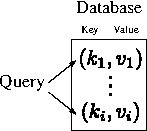
\includegraphics[scale=2.0]{./images/transformer/attention_database.pdf}
	\caption{The most similar key will be selected by measuring a similarity between a query and a key.}
\end{figure}

\begin{figure}[h]
	\centering
	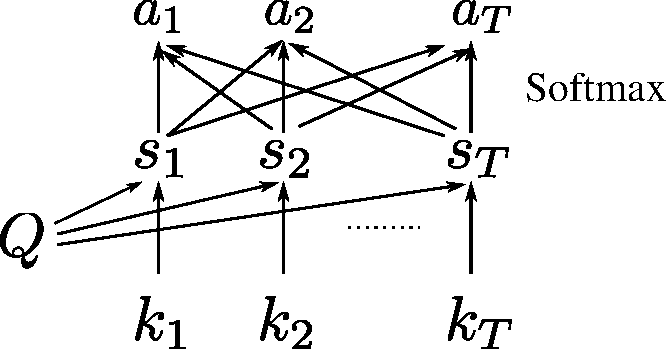
\includegraphics[scale=0.8]{./images/transformer/attention.pdf}
	\caption{The similarity $s_t$ is computed by a query and keys}
\end{figure}
There are several choices for a similarity function.
\begin{itemize}
	\item $q^Tk_i$: dot product.
	\item $\frac{q^Tk_i}{\sqrt{d}}$: scaled dot product.
	\item $q^TWk_i$: general dot product.
	\item $w_q^Tq+ w_k^Tk_i$: additive similarity.
\end{itemize}
Finally, the attention score can be computed by using a softmax:
$$a_i = \frac{\exp(s_i)}{\sum_j \exp(s_j)}$$

\section{Transformer}
\label{sec:nlp_transformer}

Attention:
$$attn(Q,K,V) = softmax(\frac{Q^TK}{\sqrt{d_k}})V$$
Masked attention:
$$\textrm{MA}(Q,K,V) = softmax\bigg(\frac{Q^TK+M}{\sqrt{d_k}}\bigg)V,$$
where $M$ is a matrix of 0 and $-\infty$. Note that $-\infty$ will make $exp$ term to be zero.





\backmatter
% bibliography, glossary and index would go here.

\nocite{*}
\bibliographystyle{unsrt}
\bibliography{references}
\end{document}
